\section[Concentration Profiles and Angular synchronization]{Factoring Out Symmetries in Concentration Profiles Using~Angular~Synchronization}

\begin{frame}{Importance of Symmetries in Data Analysis}

	\centering
	In the previous analysis, we first needed to determine \\where to open and ``unroll'' the circle
	
	\centering
	\begin{tikzpicture}
		\node (drosophila_line) {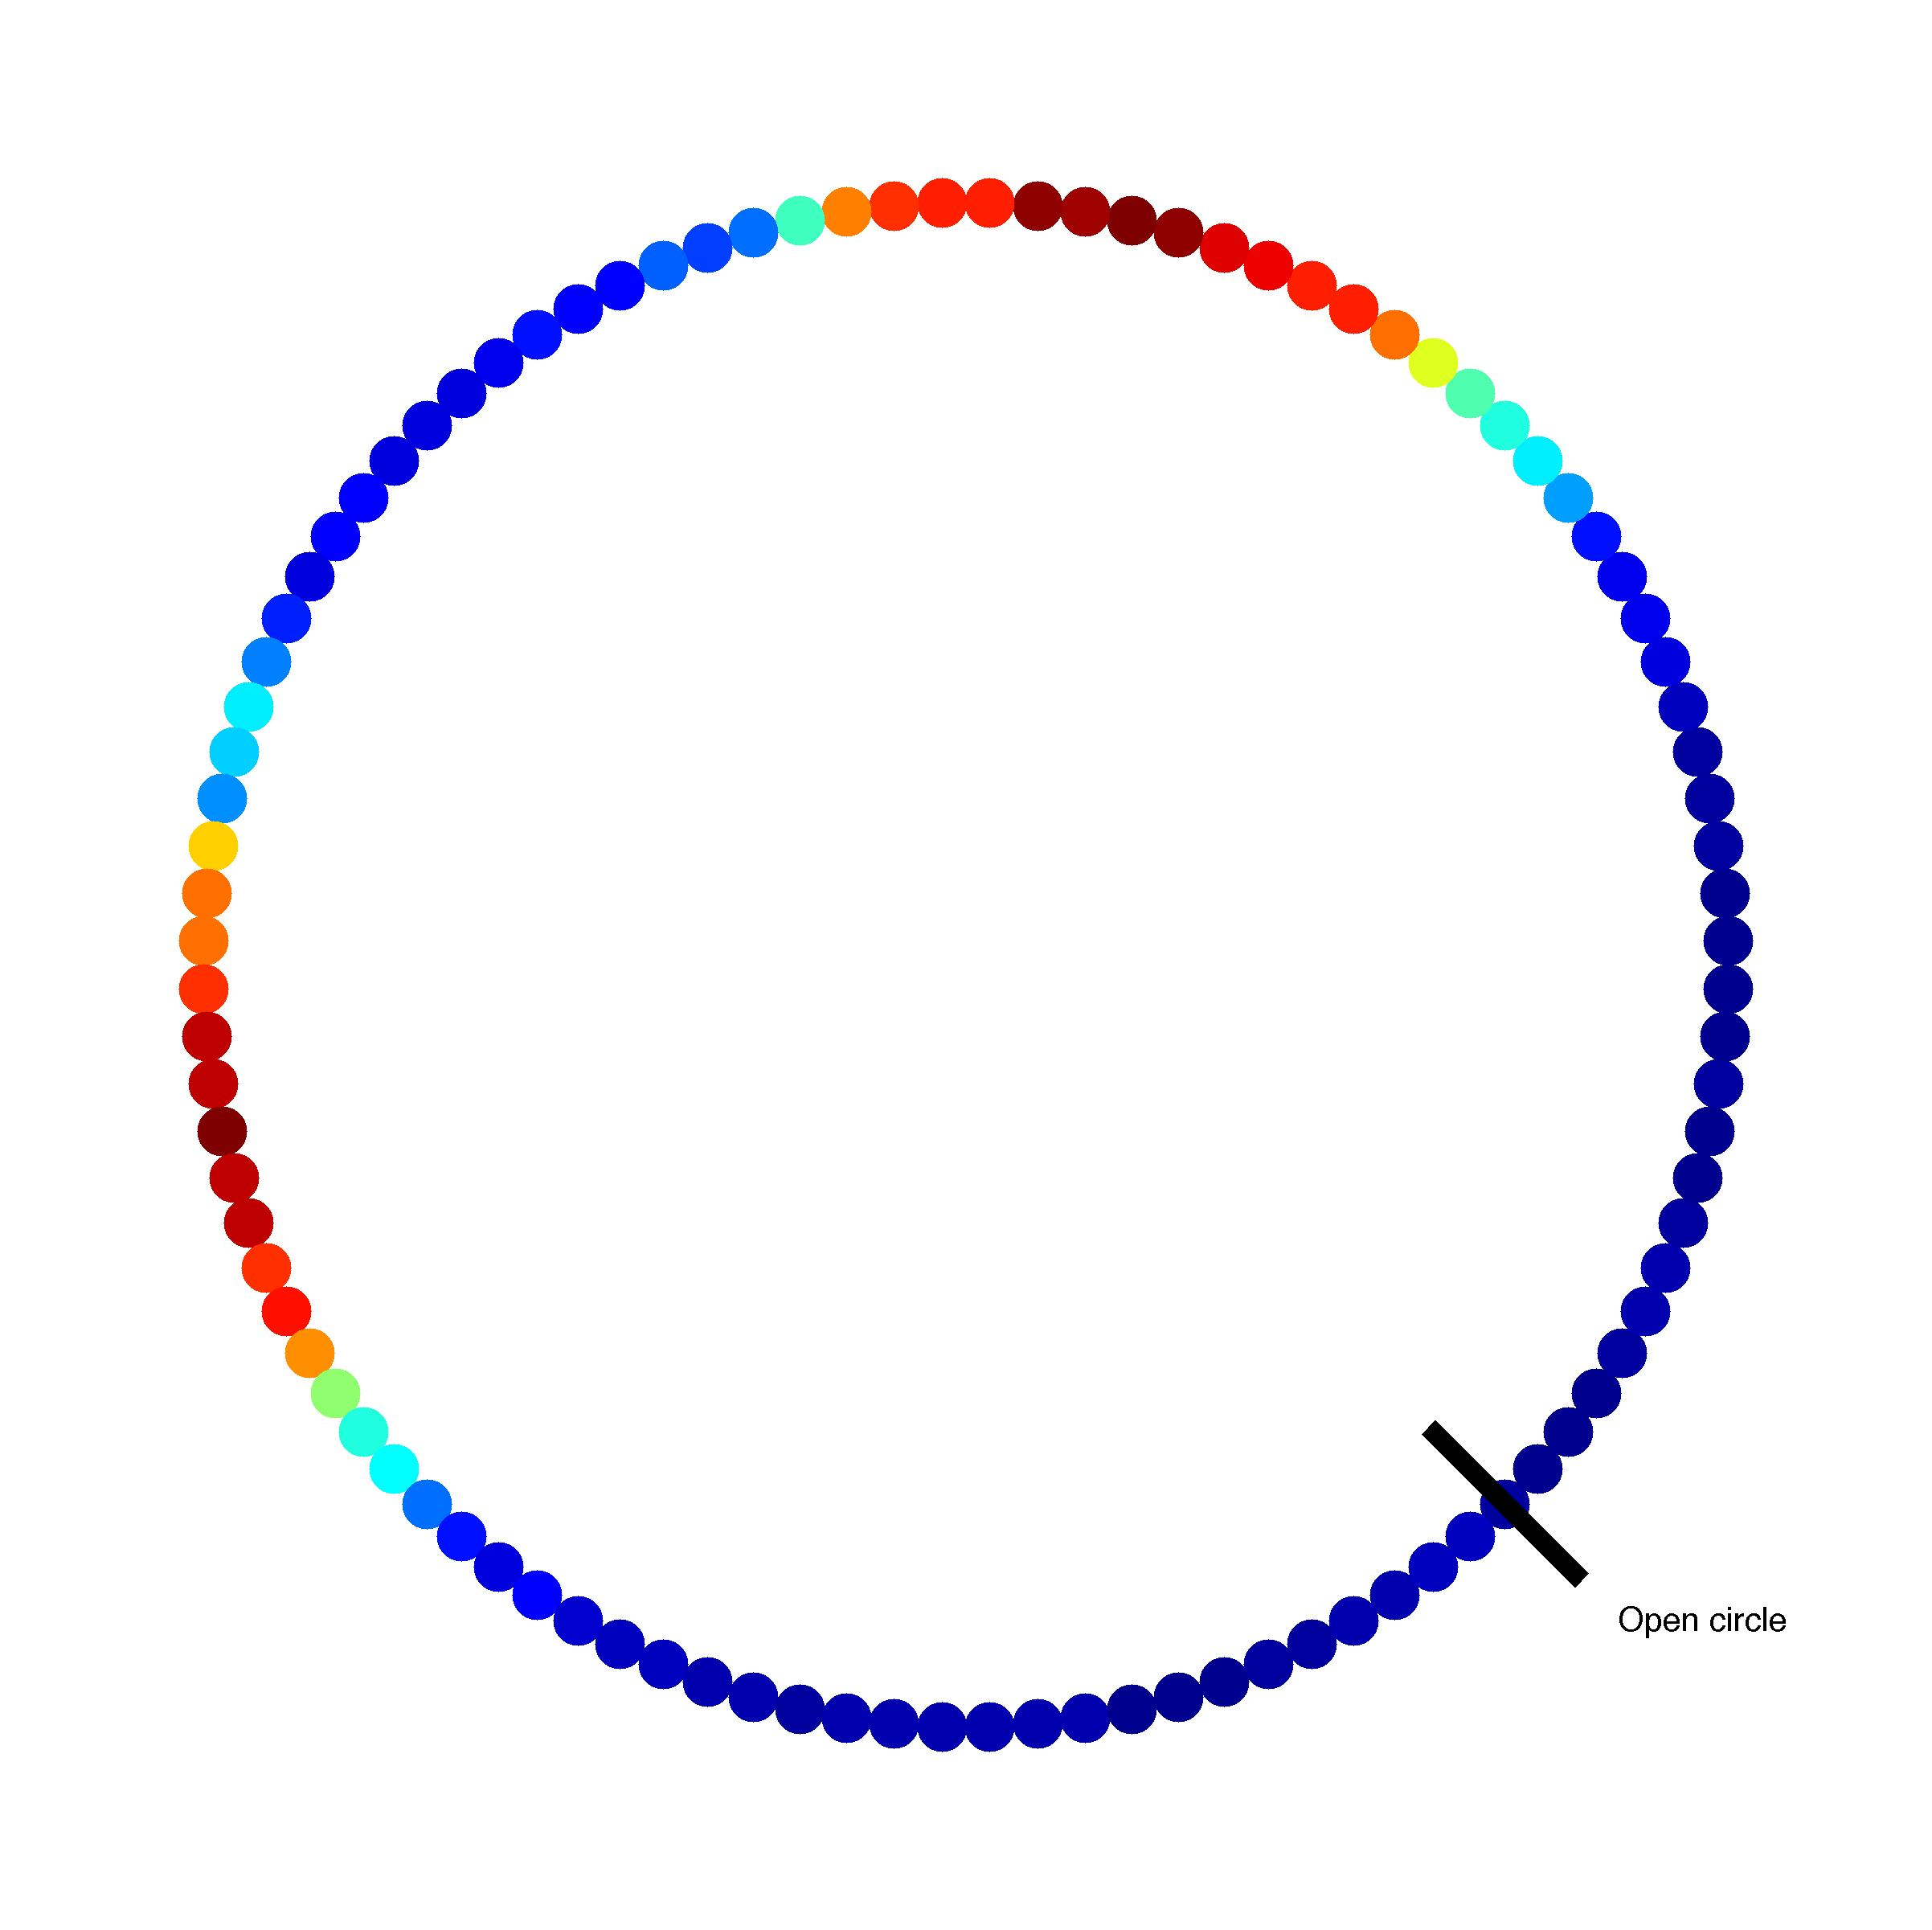
\includegraphics[width=0.2\textwidth]{circle_profile}};
		\node[right=0.3\textwidth of drosophila_line] (drosophila_circle) {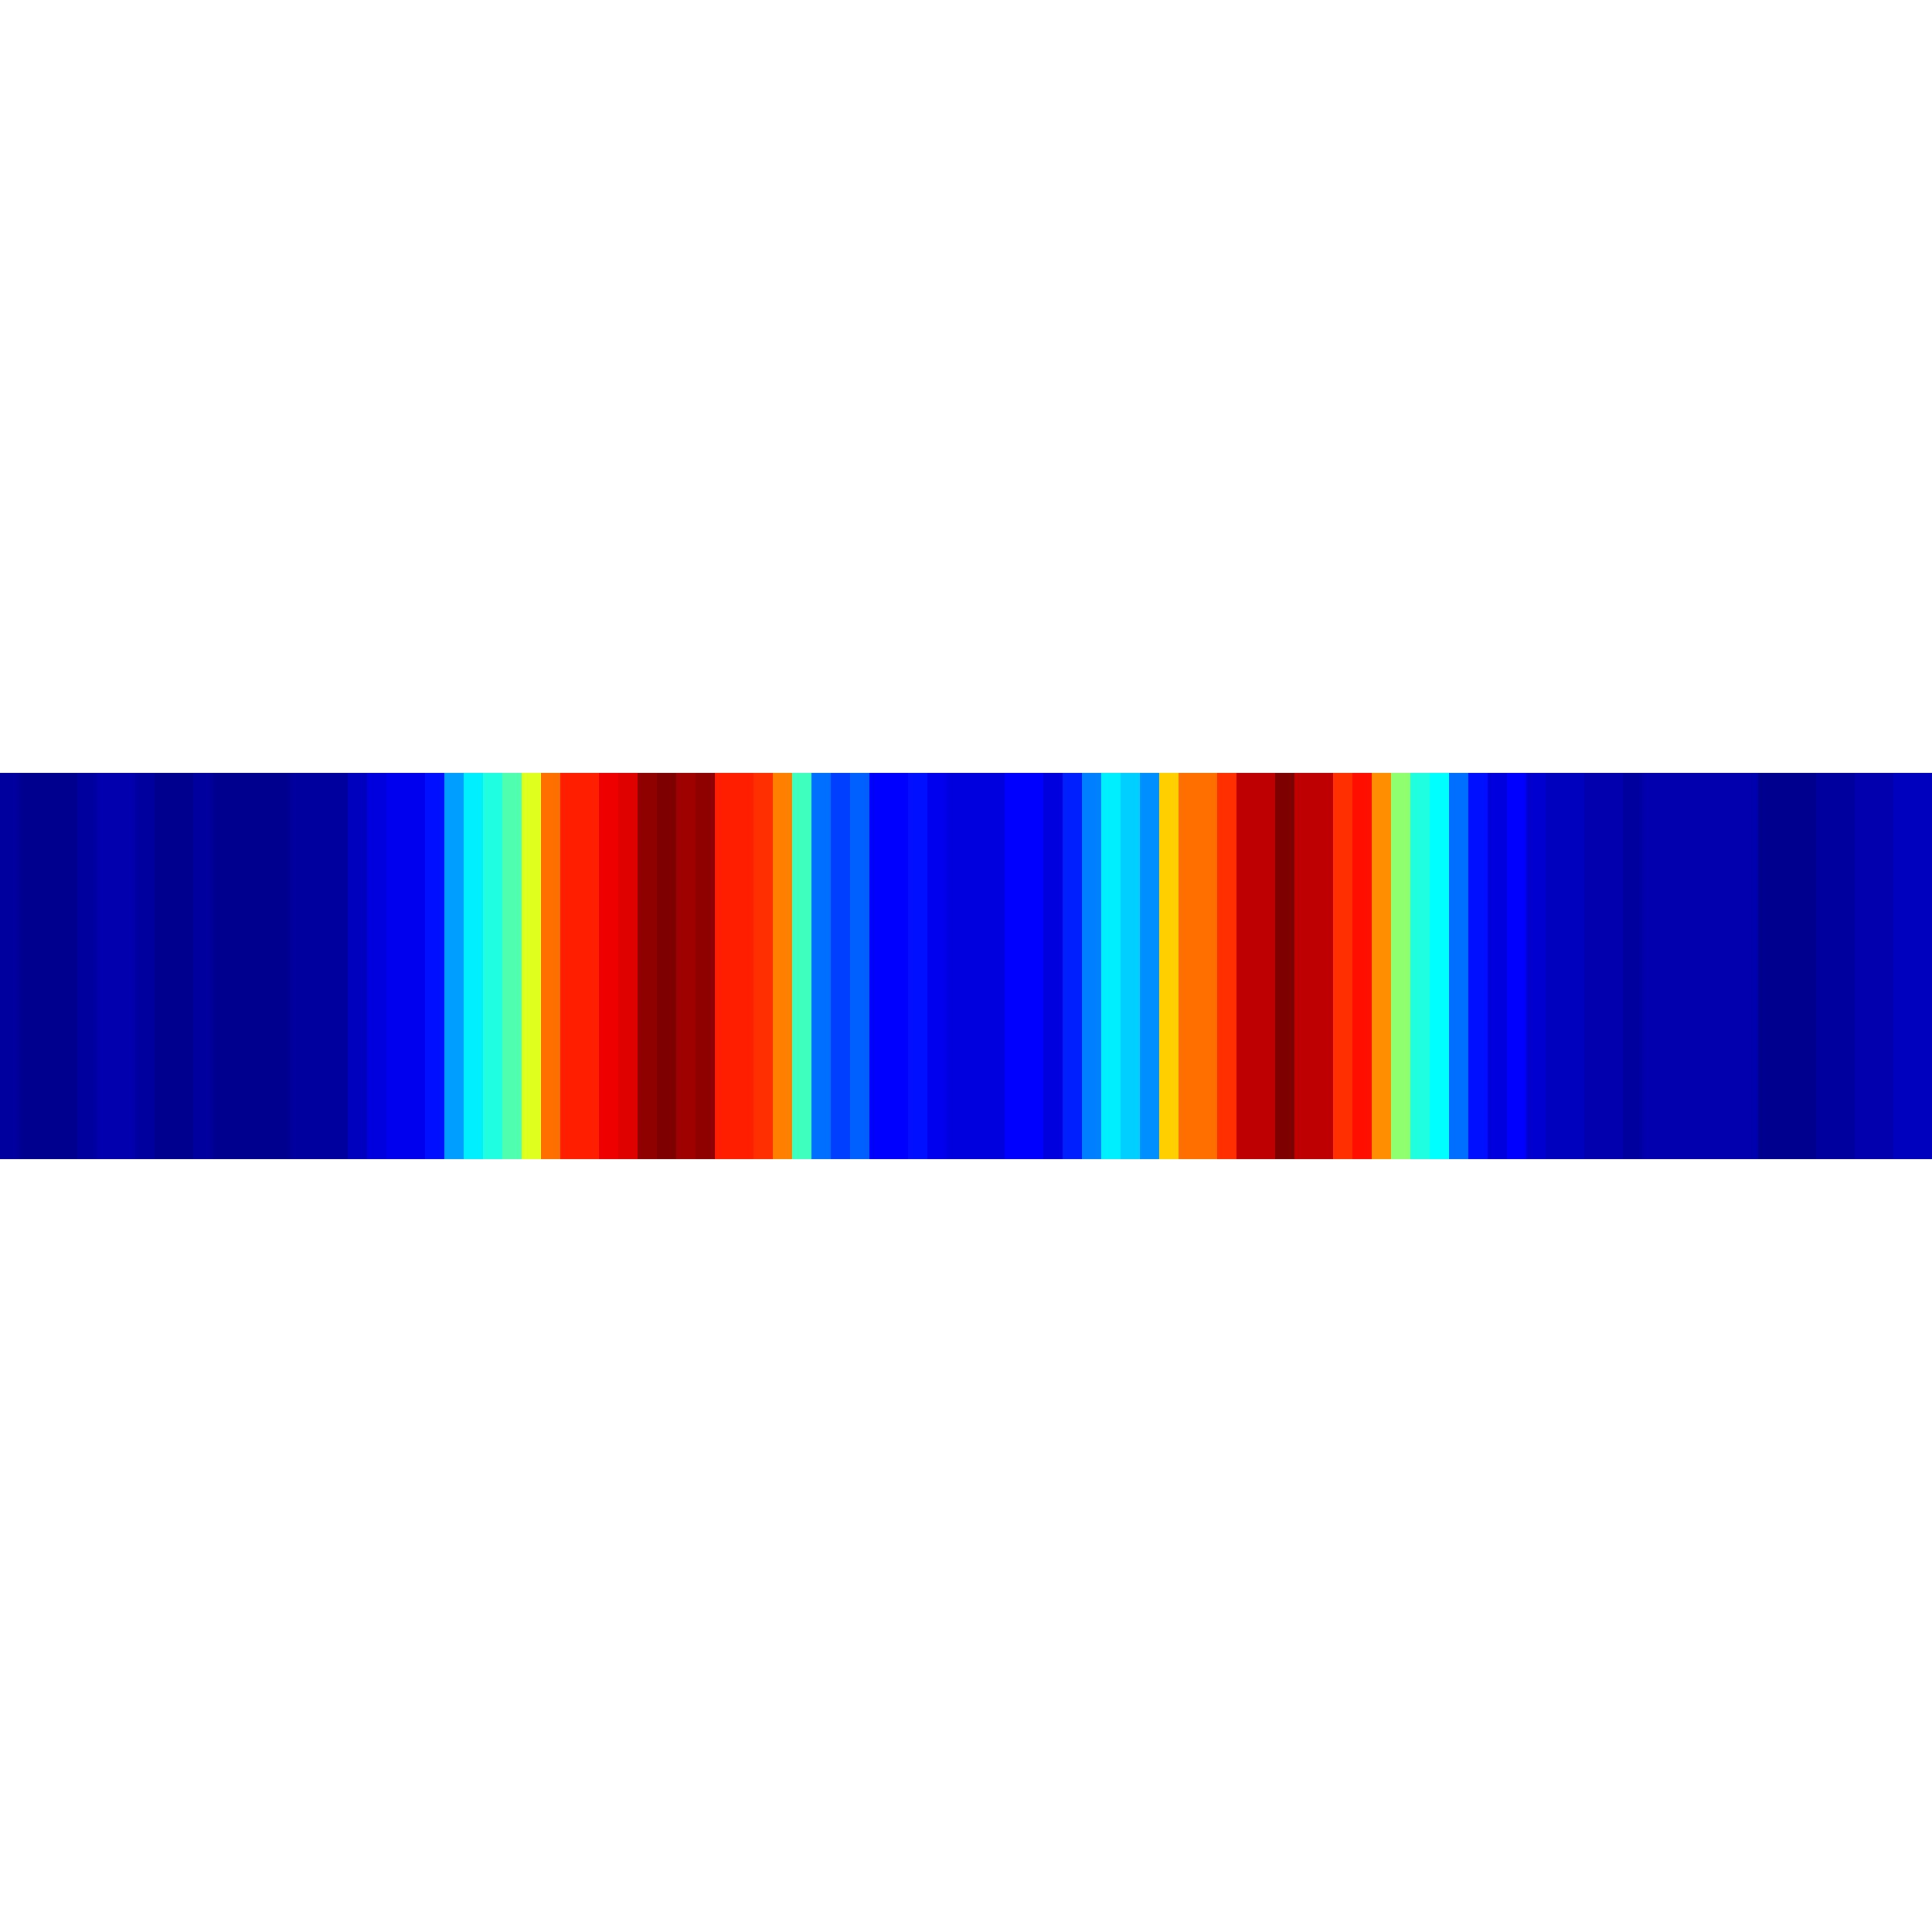
\includegraphics[width=0.25\textwidth, height=0.1in]{line_profile}};
		\draw[->] (drosophila_line) -- (drosophila_circle) node[above,midway] {``Unroll'' circle};
	\end{tikzpicture}
	
	This is done by staining for {\em another} protein that is expressed only along the ventral midline, and then aligning the profiles along their ventral midlines
	
	\vspace{0.2in}
	We would like to {\em automatically} align these concentration profiles\\
	without having to stain for a second protein

\end{frame}

\begin{frame}{How to Address Rotation Invariance in Data Analysis}
    There are two ways to view rotation-invariant data
 
 	\begin{block}{}
        \begin{tikzpicture}
        	\node[text width=0.3\textwidth] (text1) {{\bf We can use rotations to {\em augment} data} \\ Given a data point $x$, we include all rotations of $x$ in our data set \par};
            \node[right=of text1] (fig1) {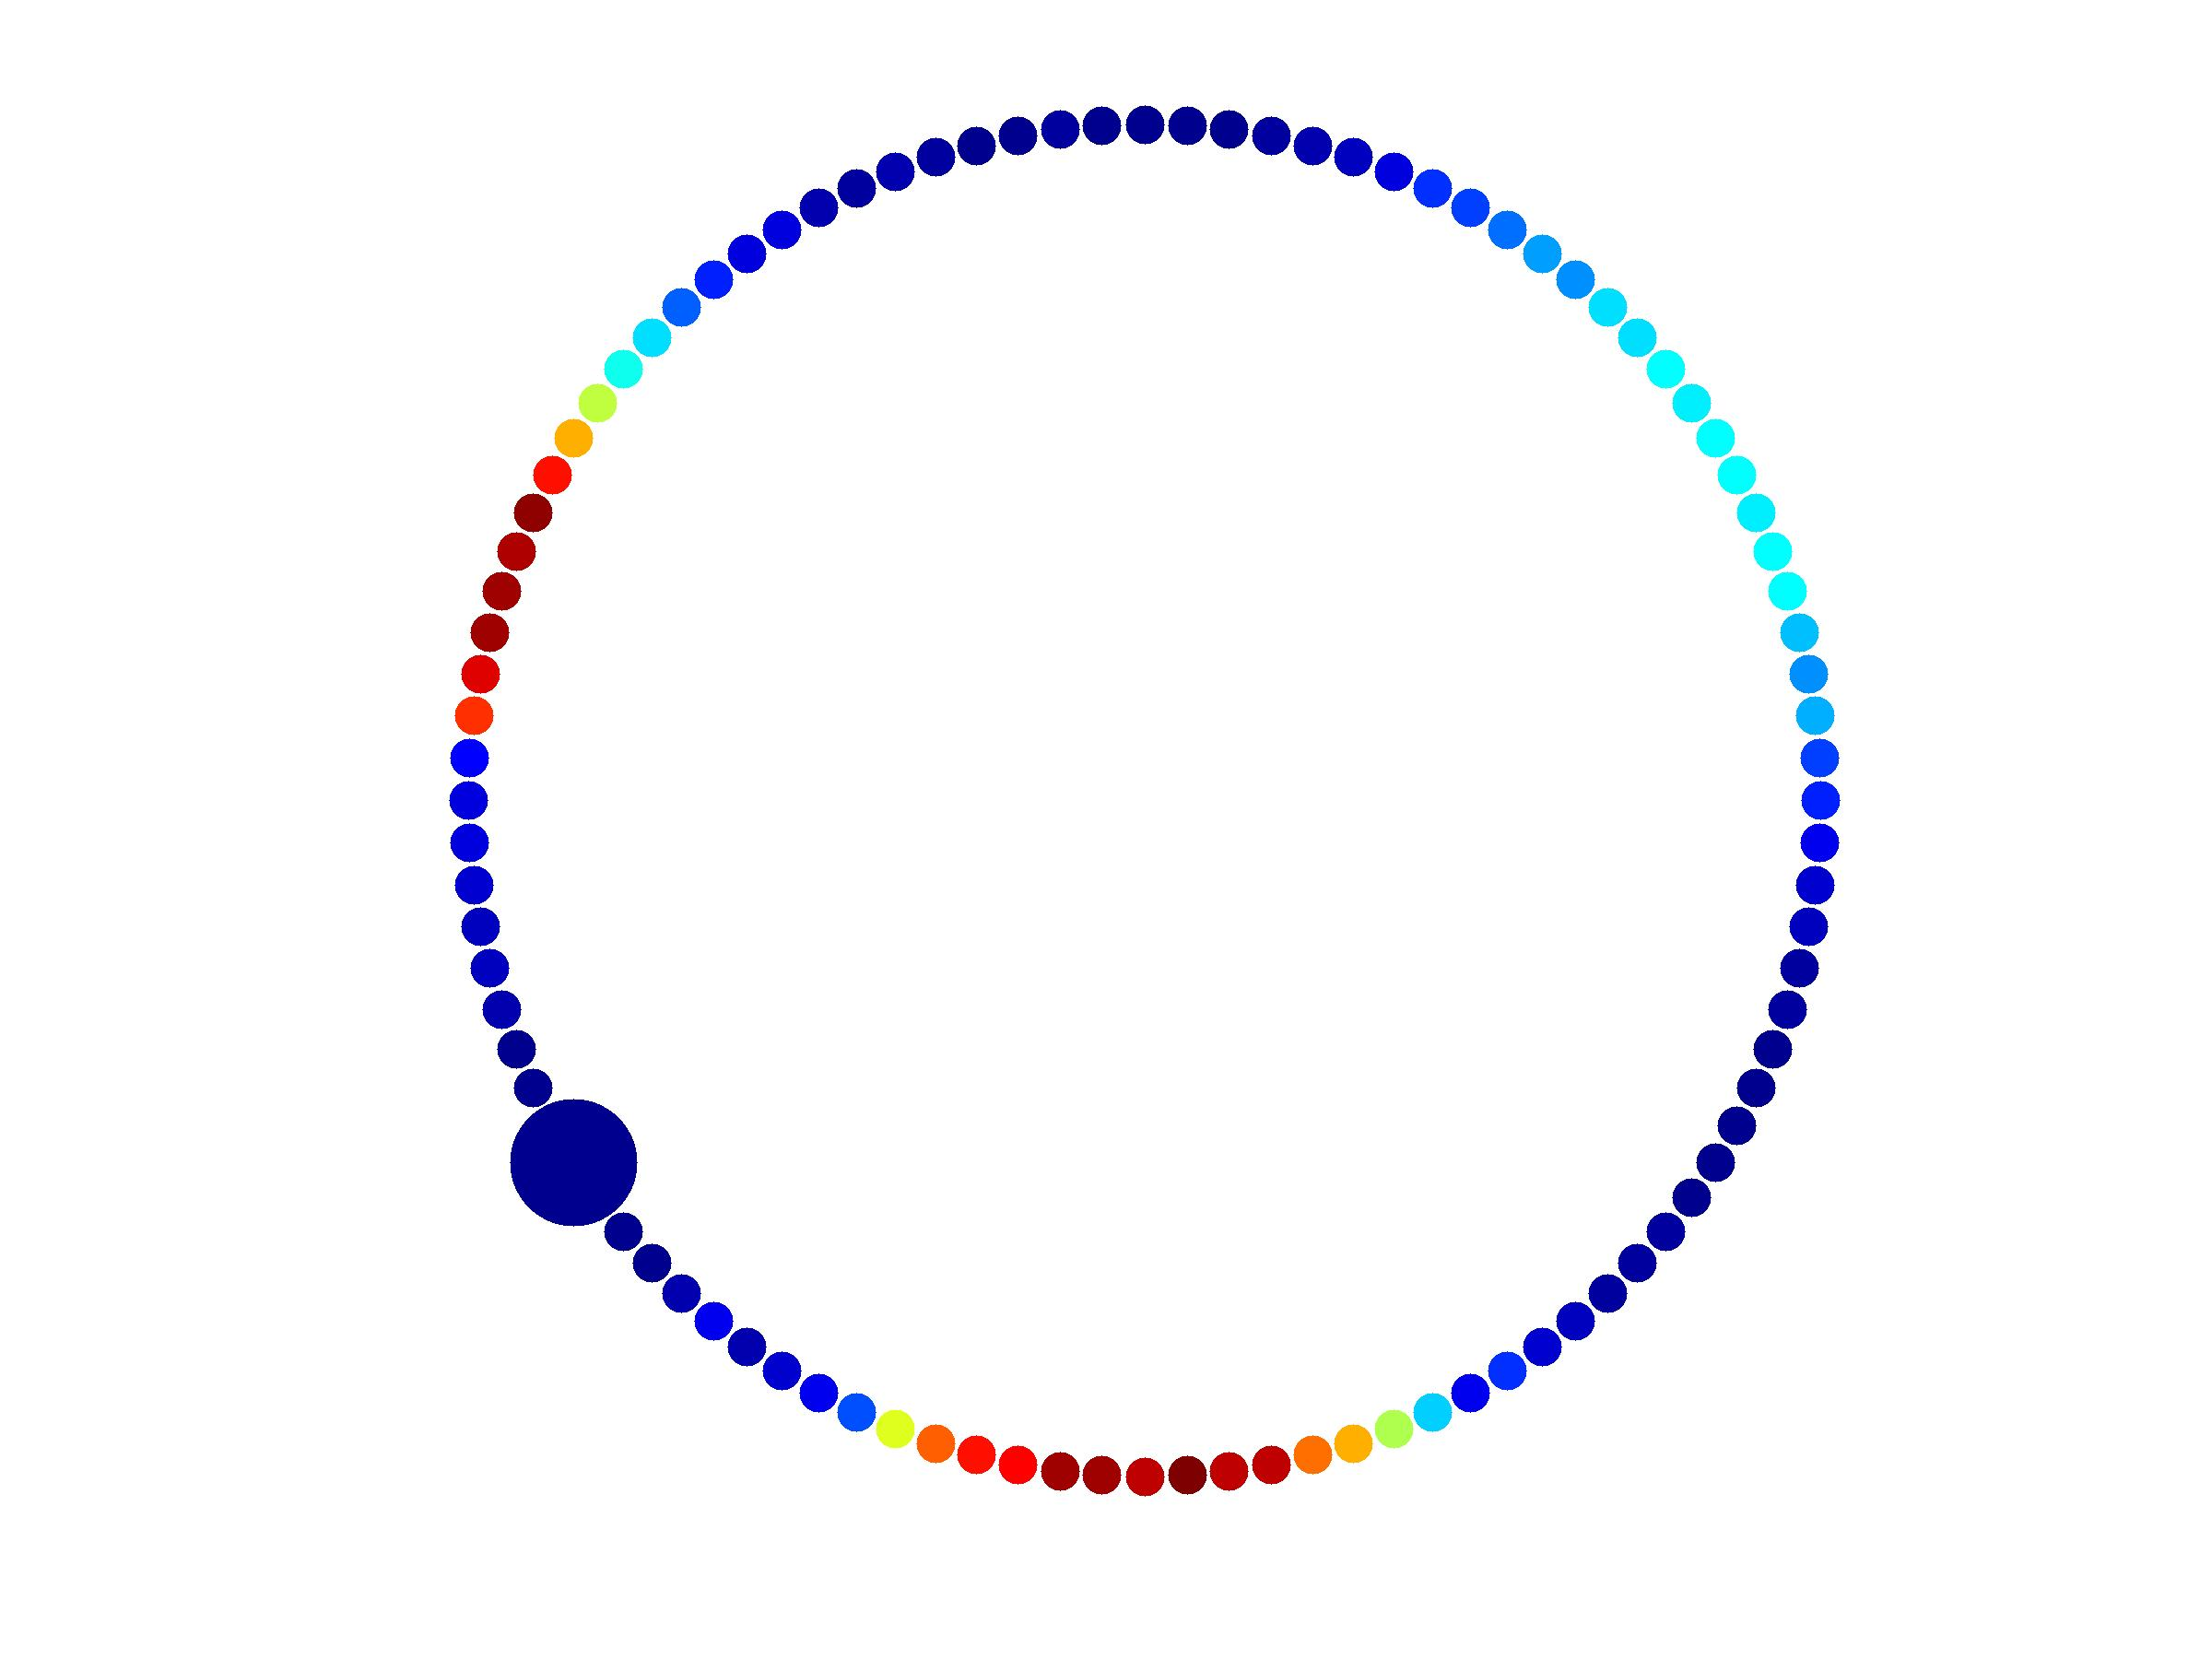
\includegraphics[width=0.25\textwidth]{../SIAM_DS_2013/drosophila_rot1.jpg}};
            \node [right of=fig1, node distance=0.35\textwidth] (fig2) {
            \begin{minipage}{0.25\textwidth}
                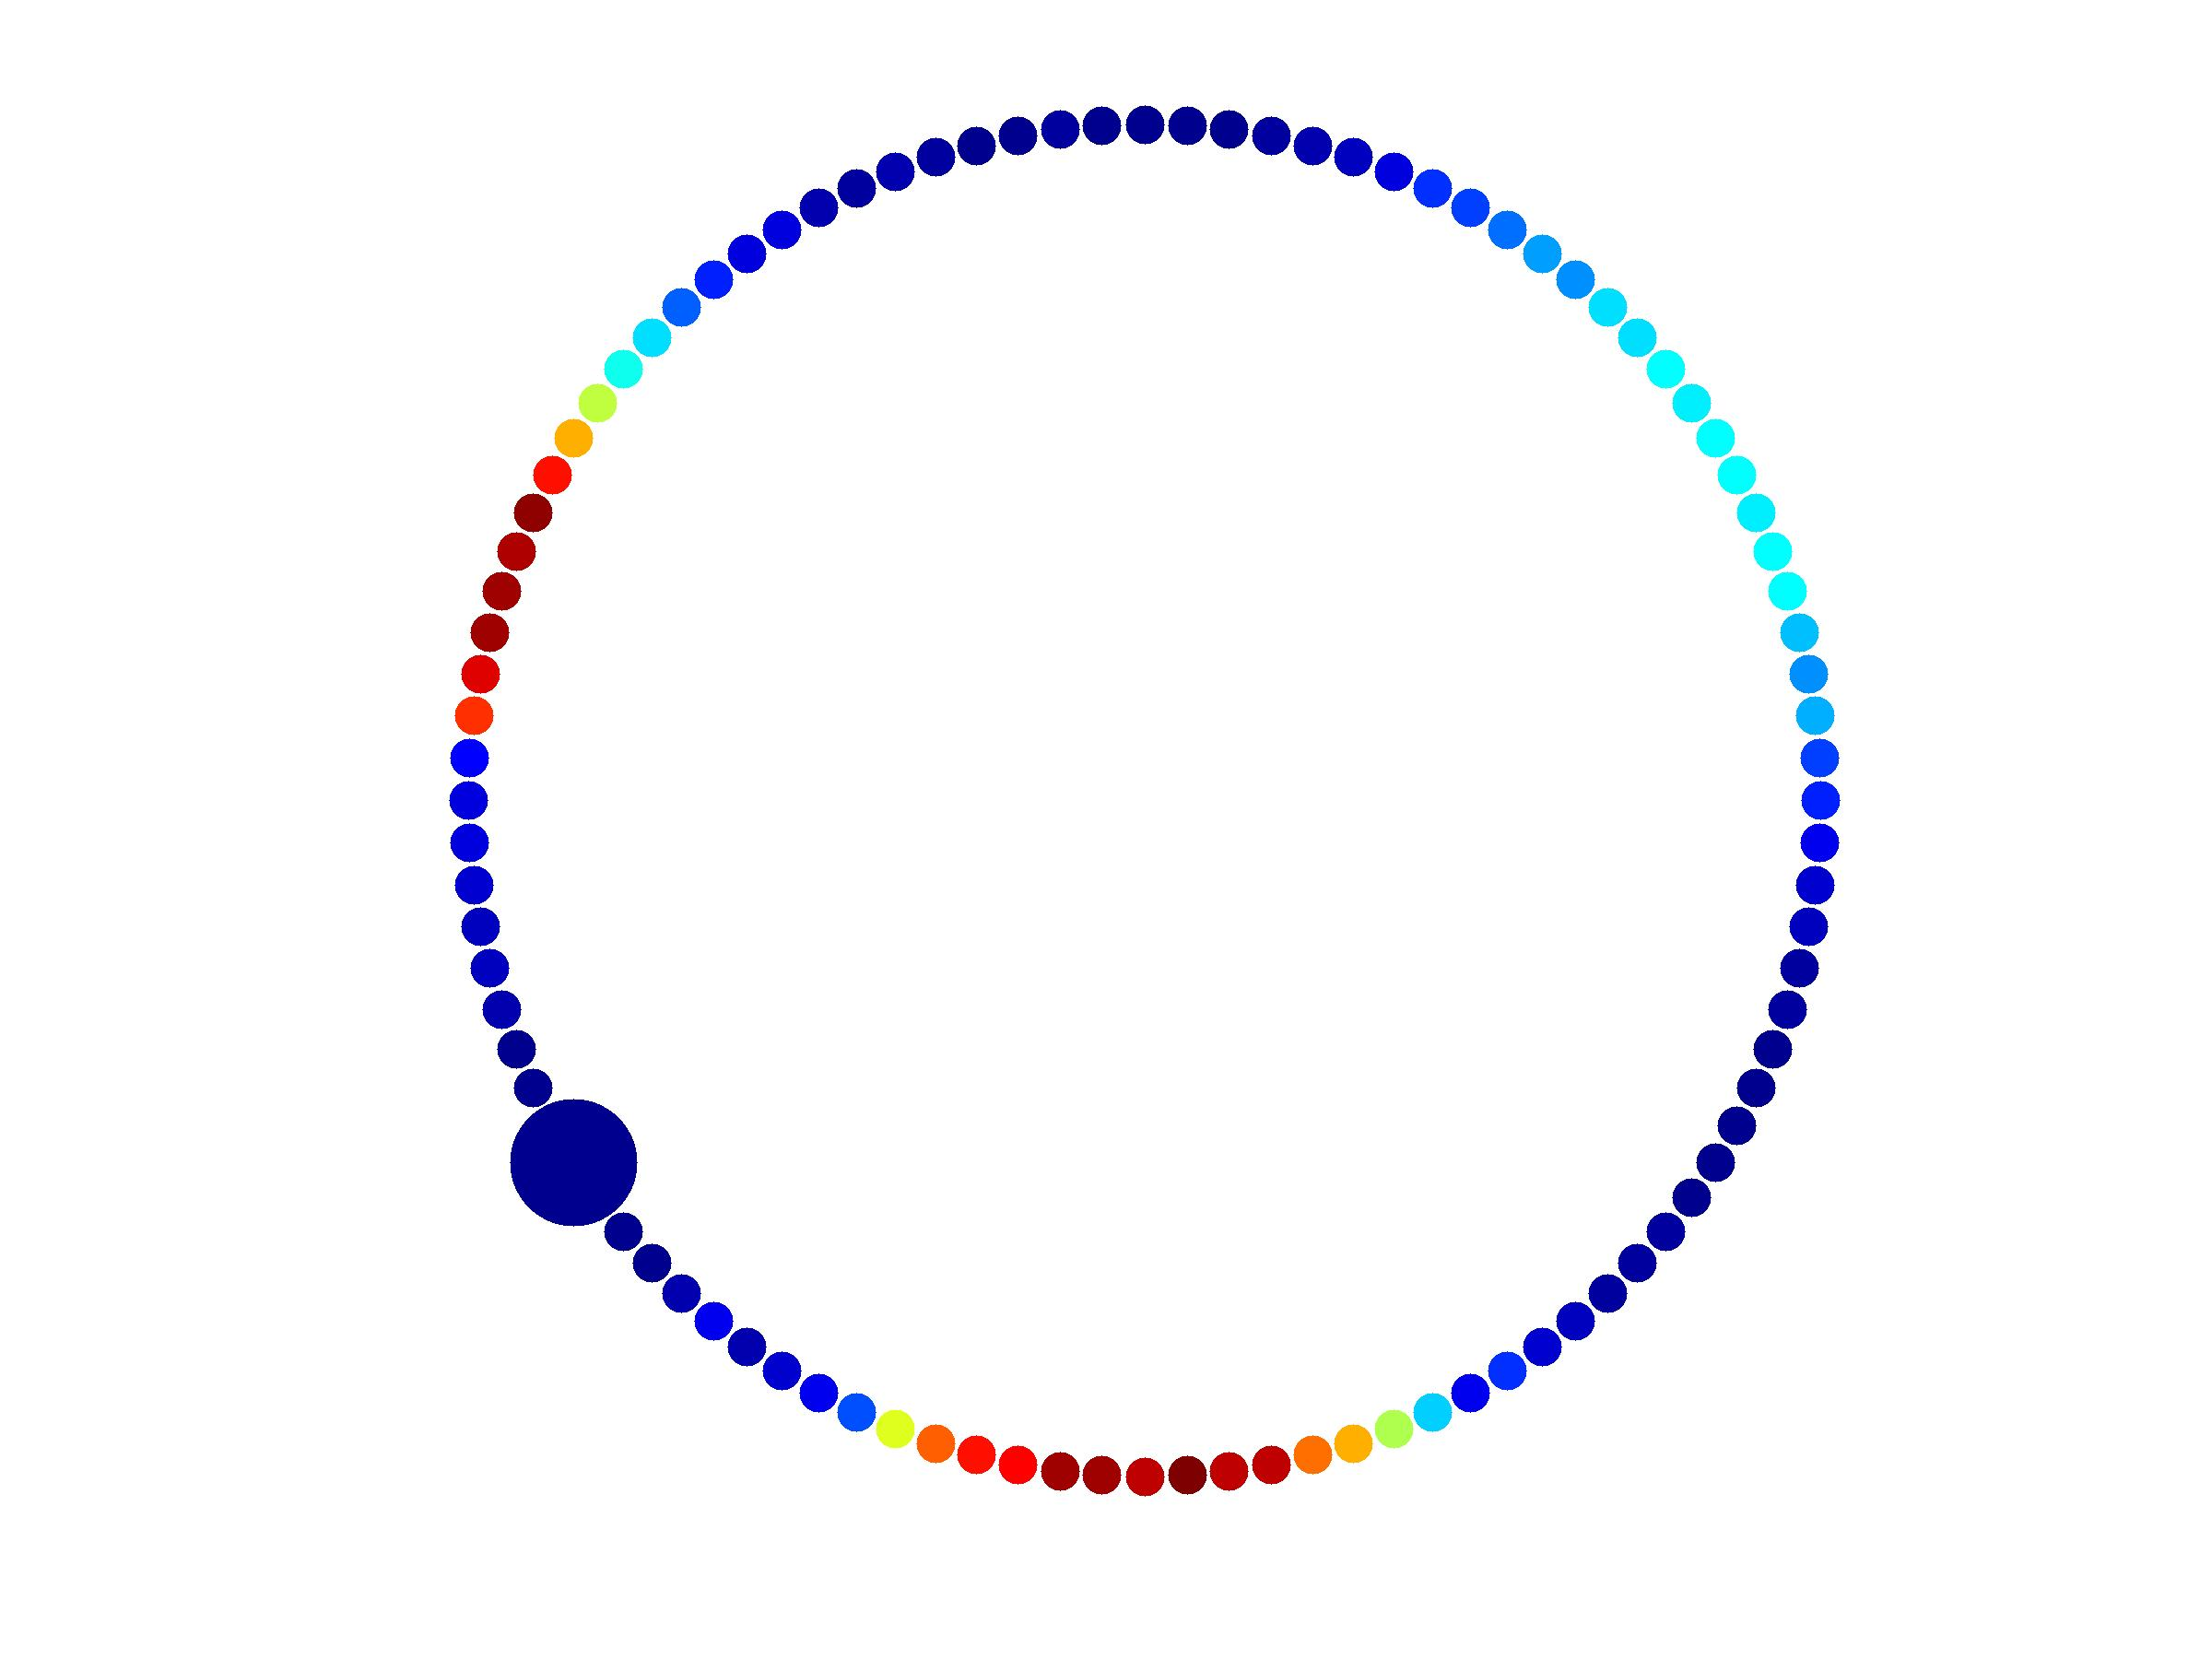
\includegraphics[width=0.45\textwidth]{../SIAM_DS_2013/drosophila_rot1.jpg}
                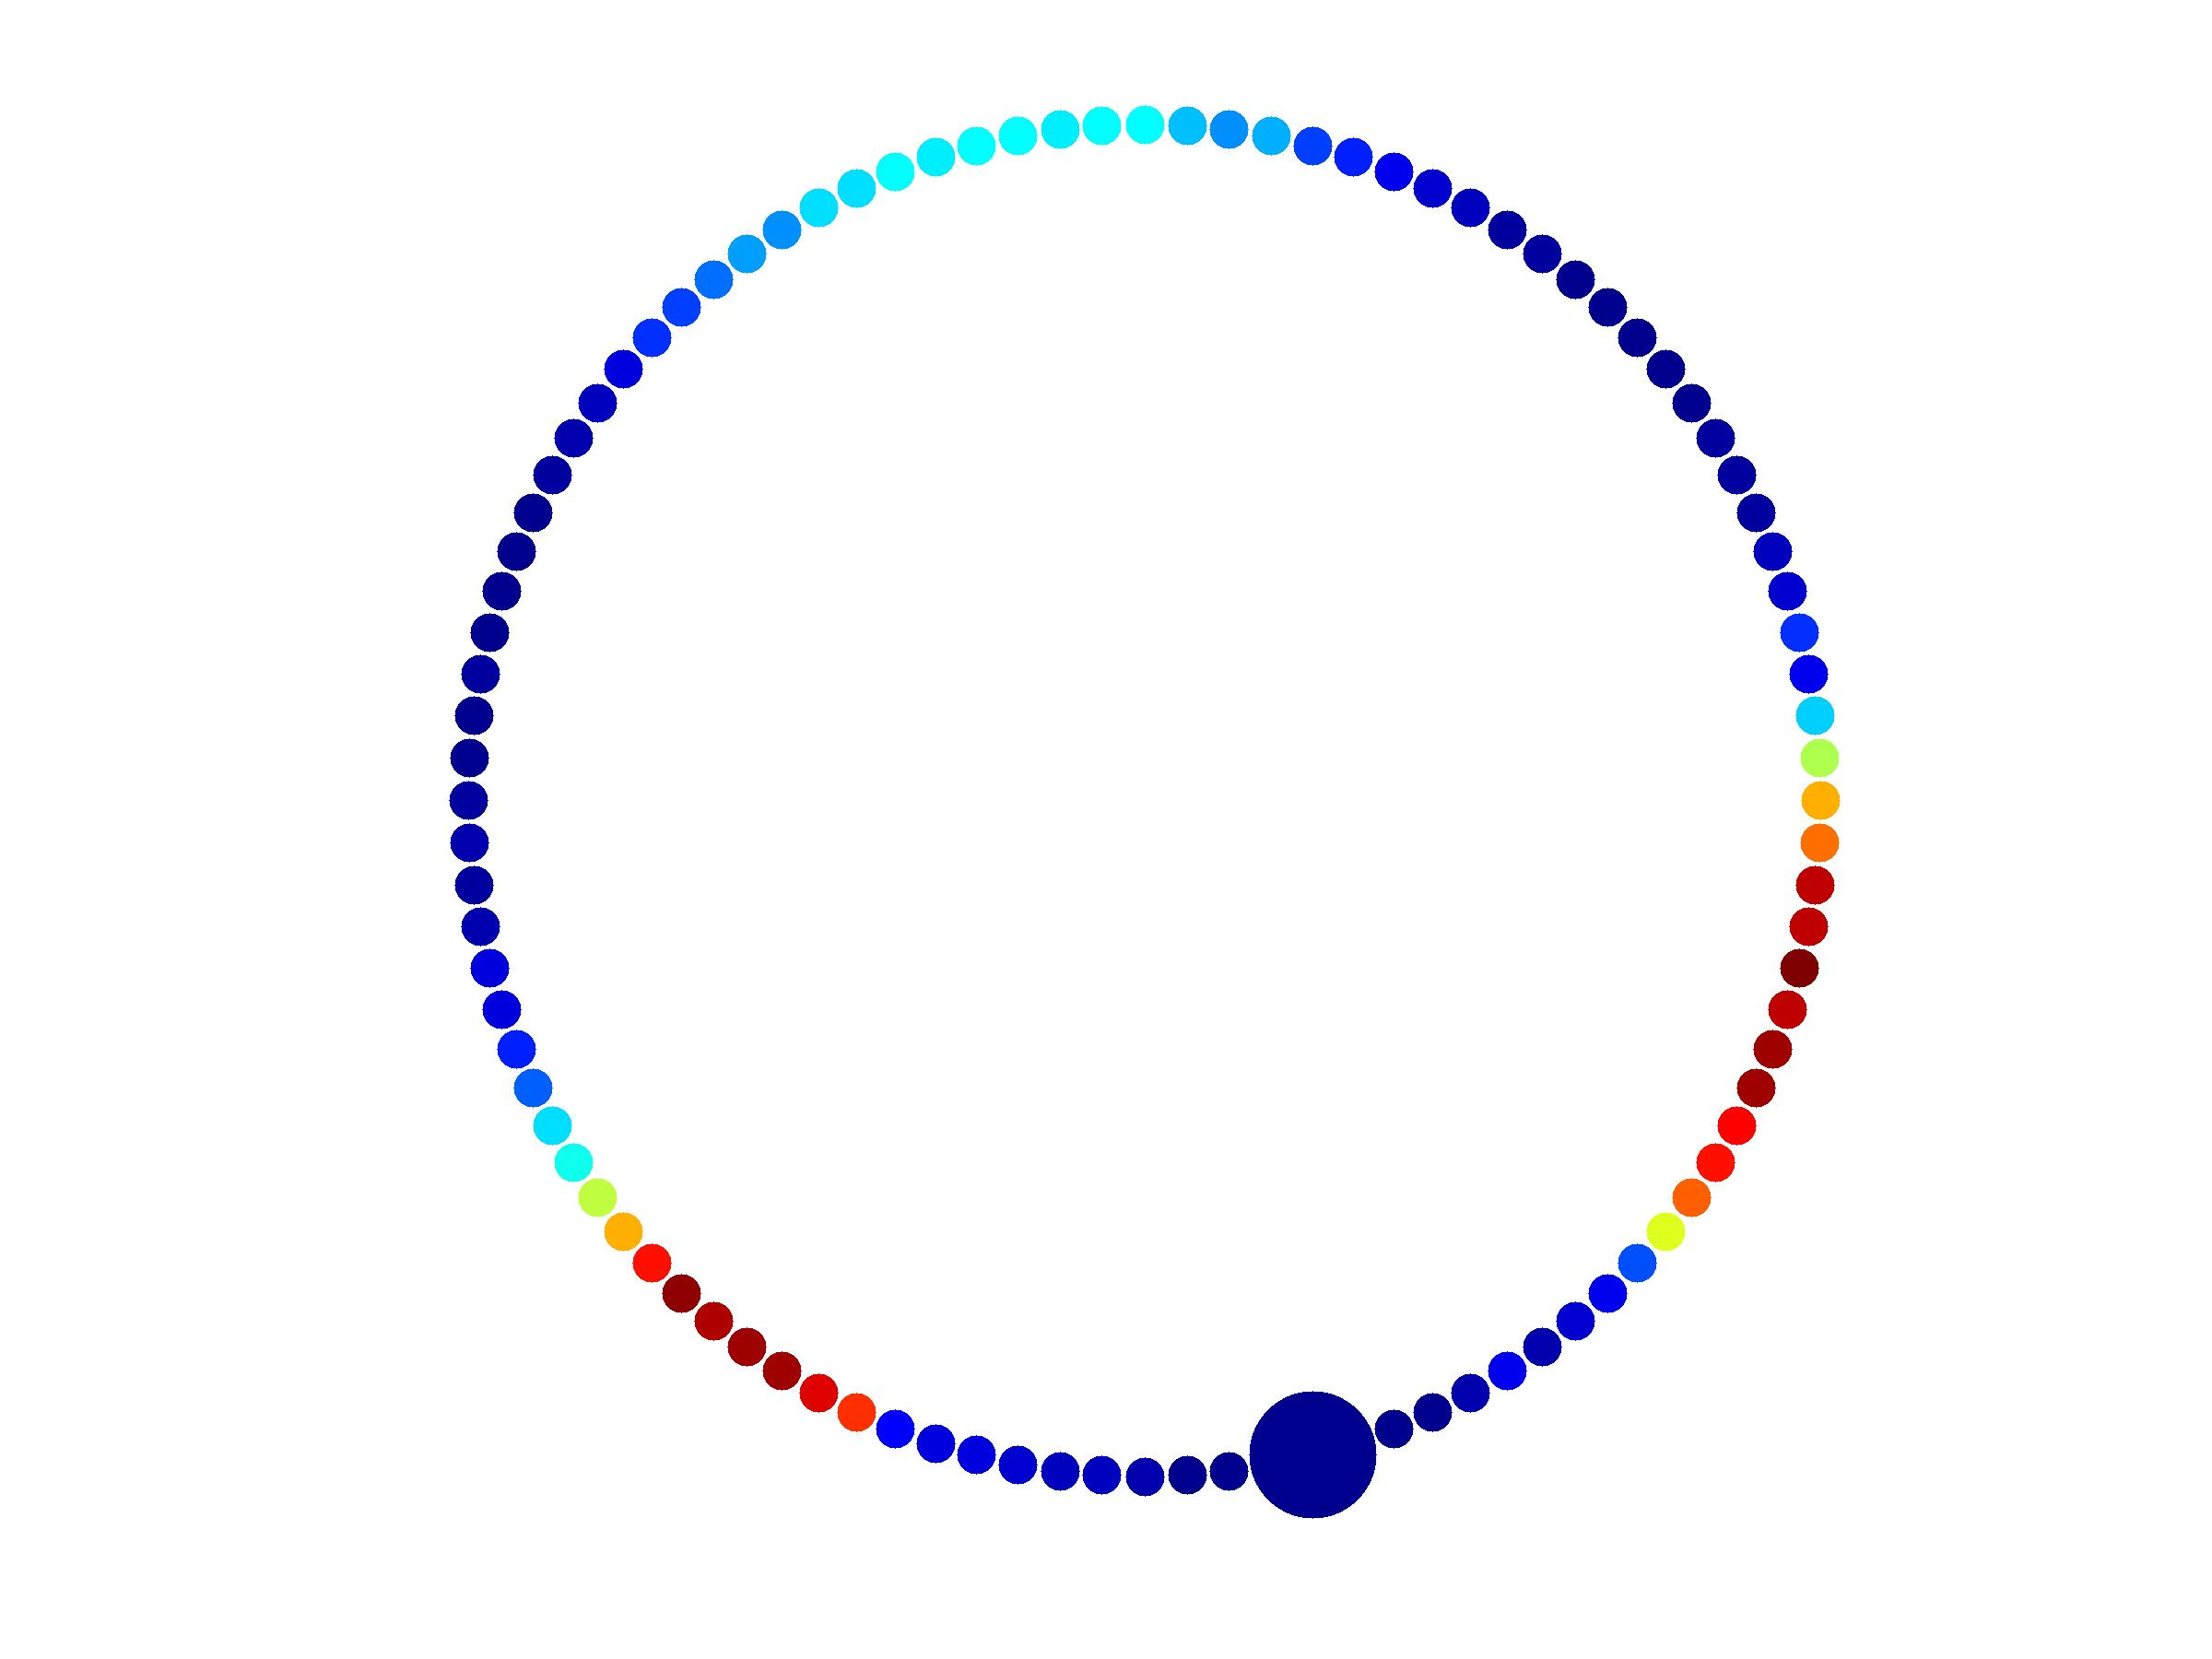
\includegraphics[width=0.45\textwidth]{../SIAM_DS_2013/drosophila_rot3.jpg}\\
                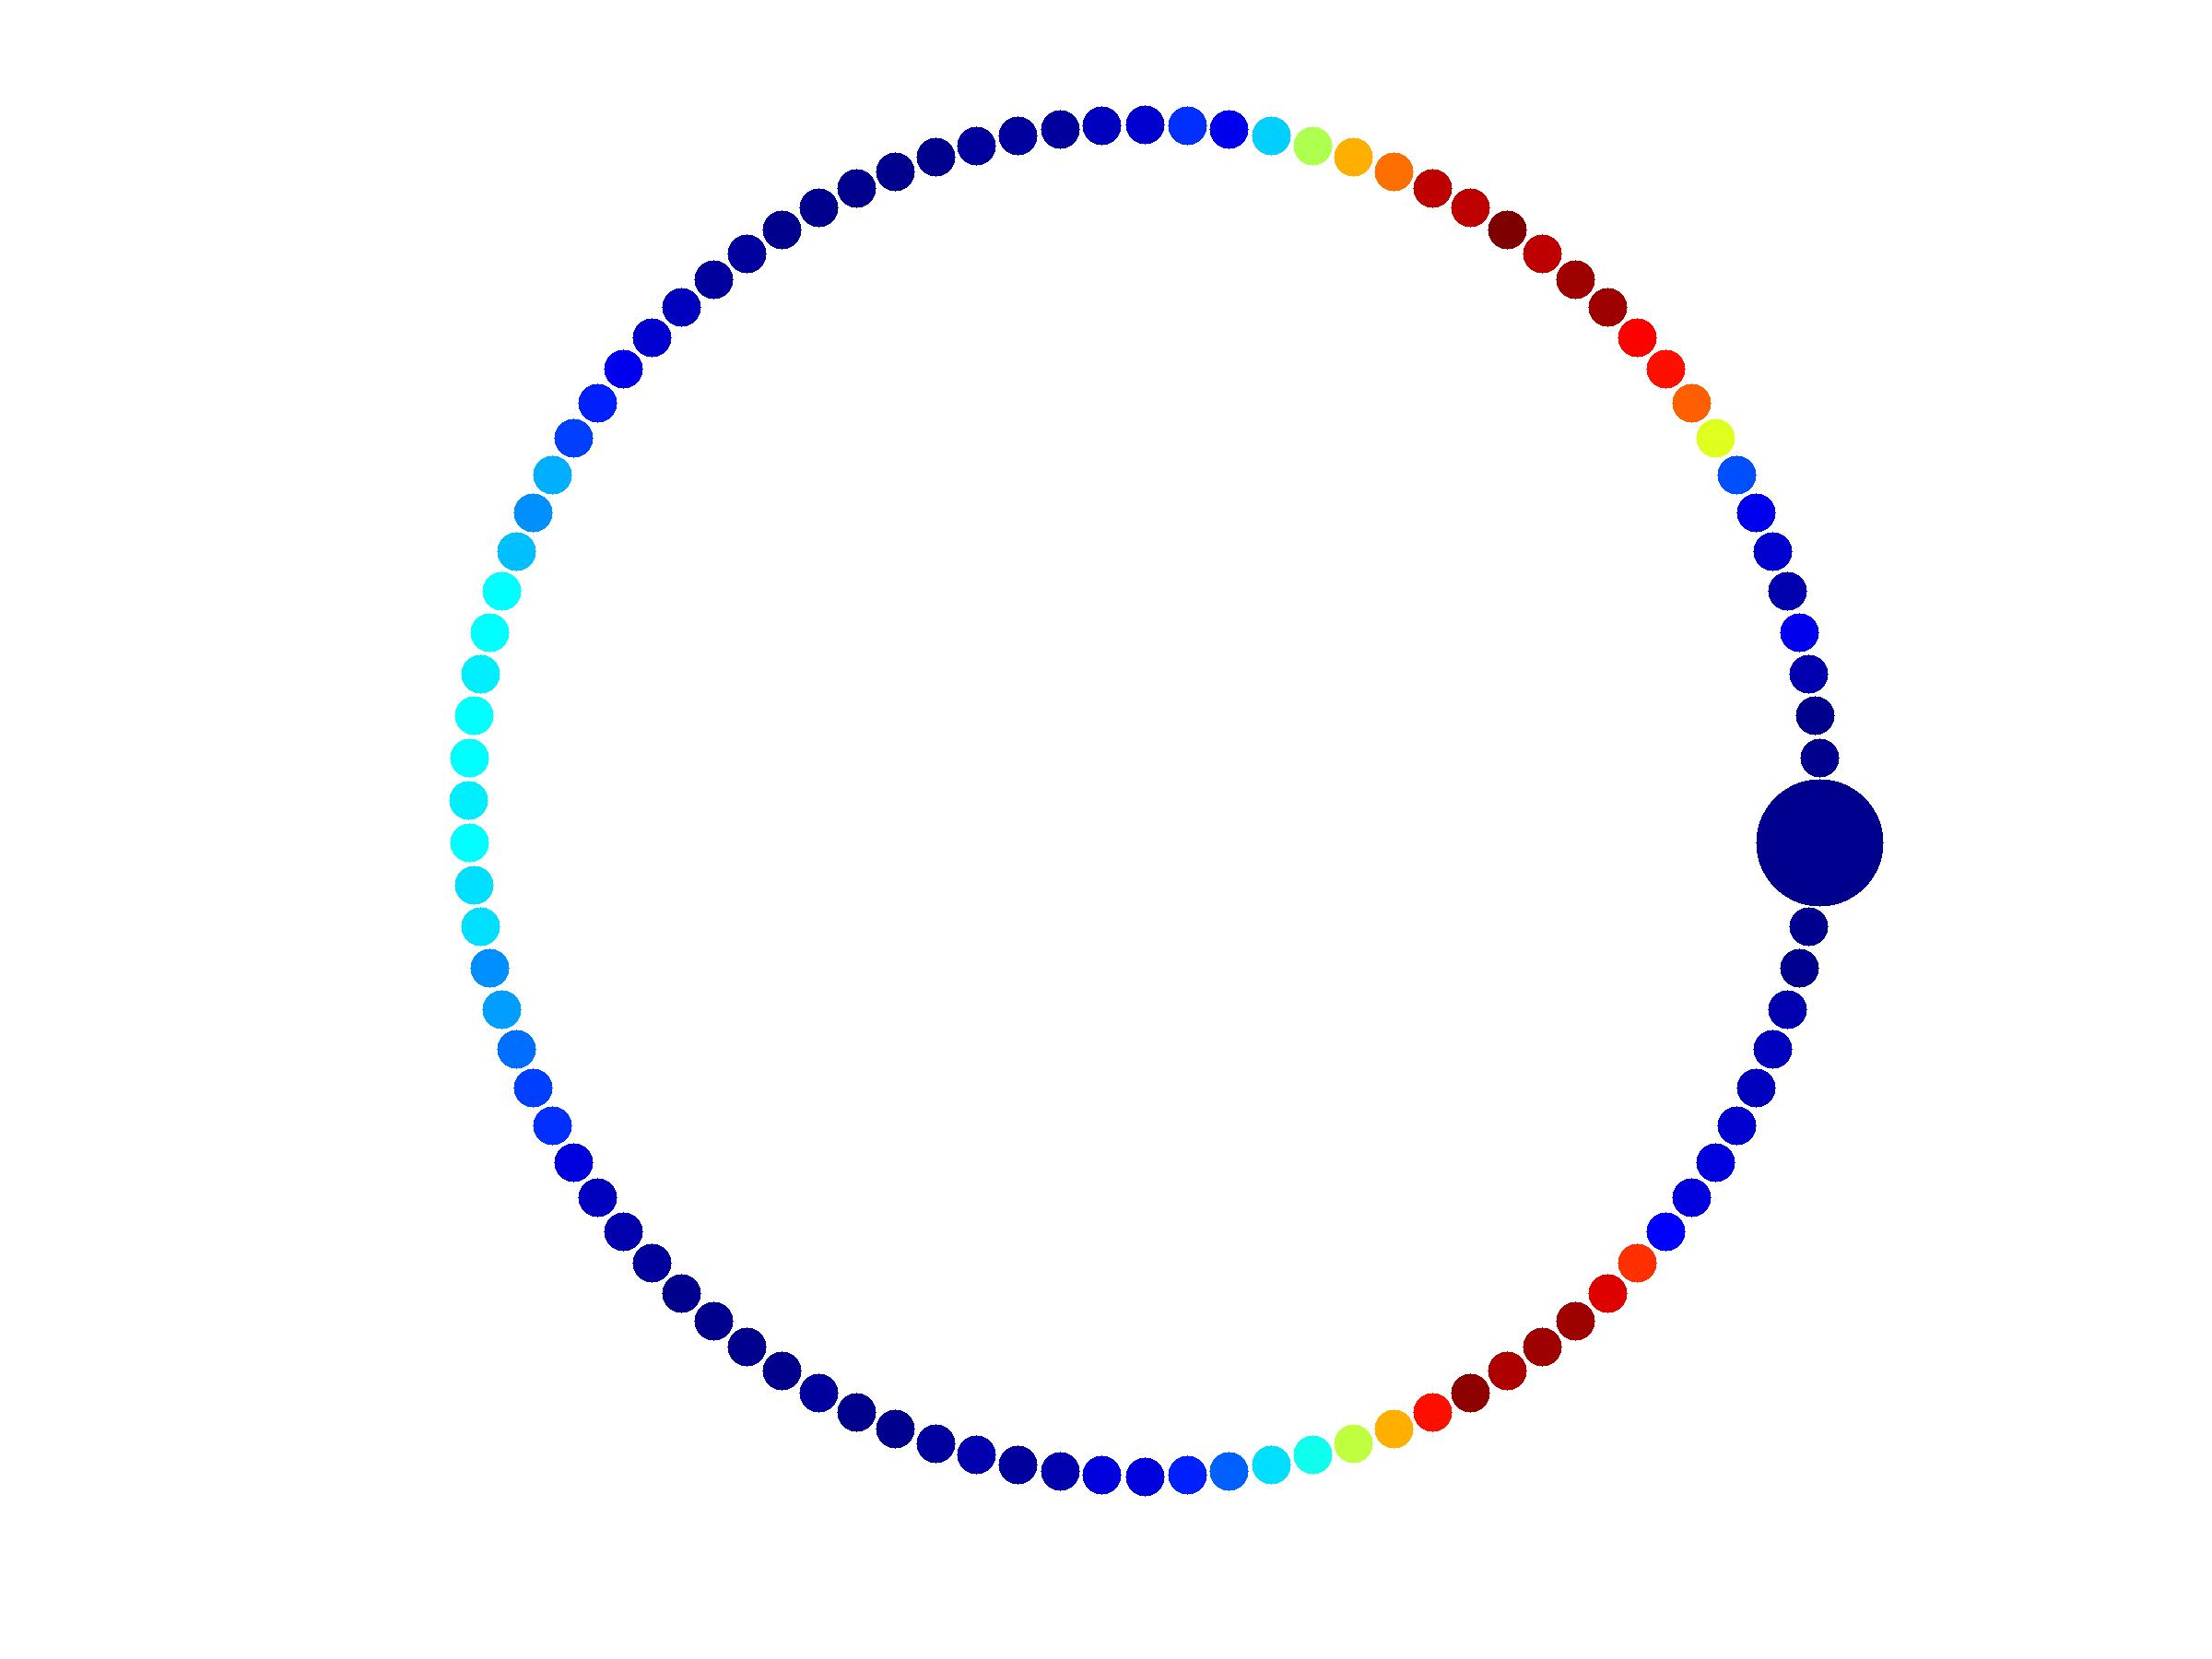
\includegraphics[width=0.45\textwidth]{../SIAM_DS_2013/drosophila_rot5.jpg}
                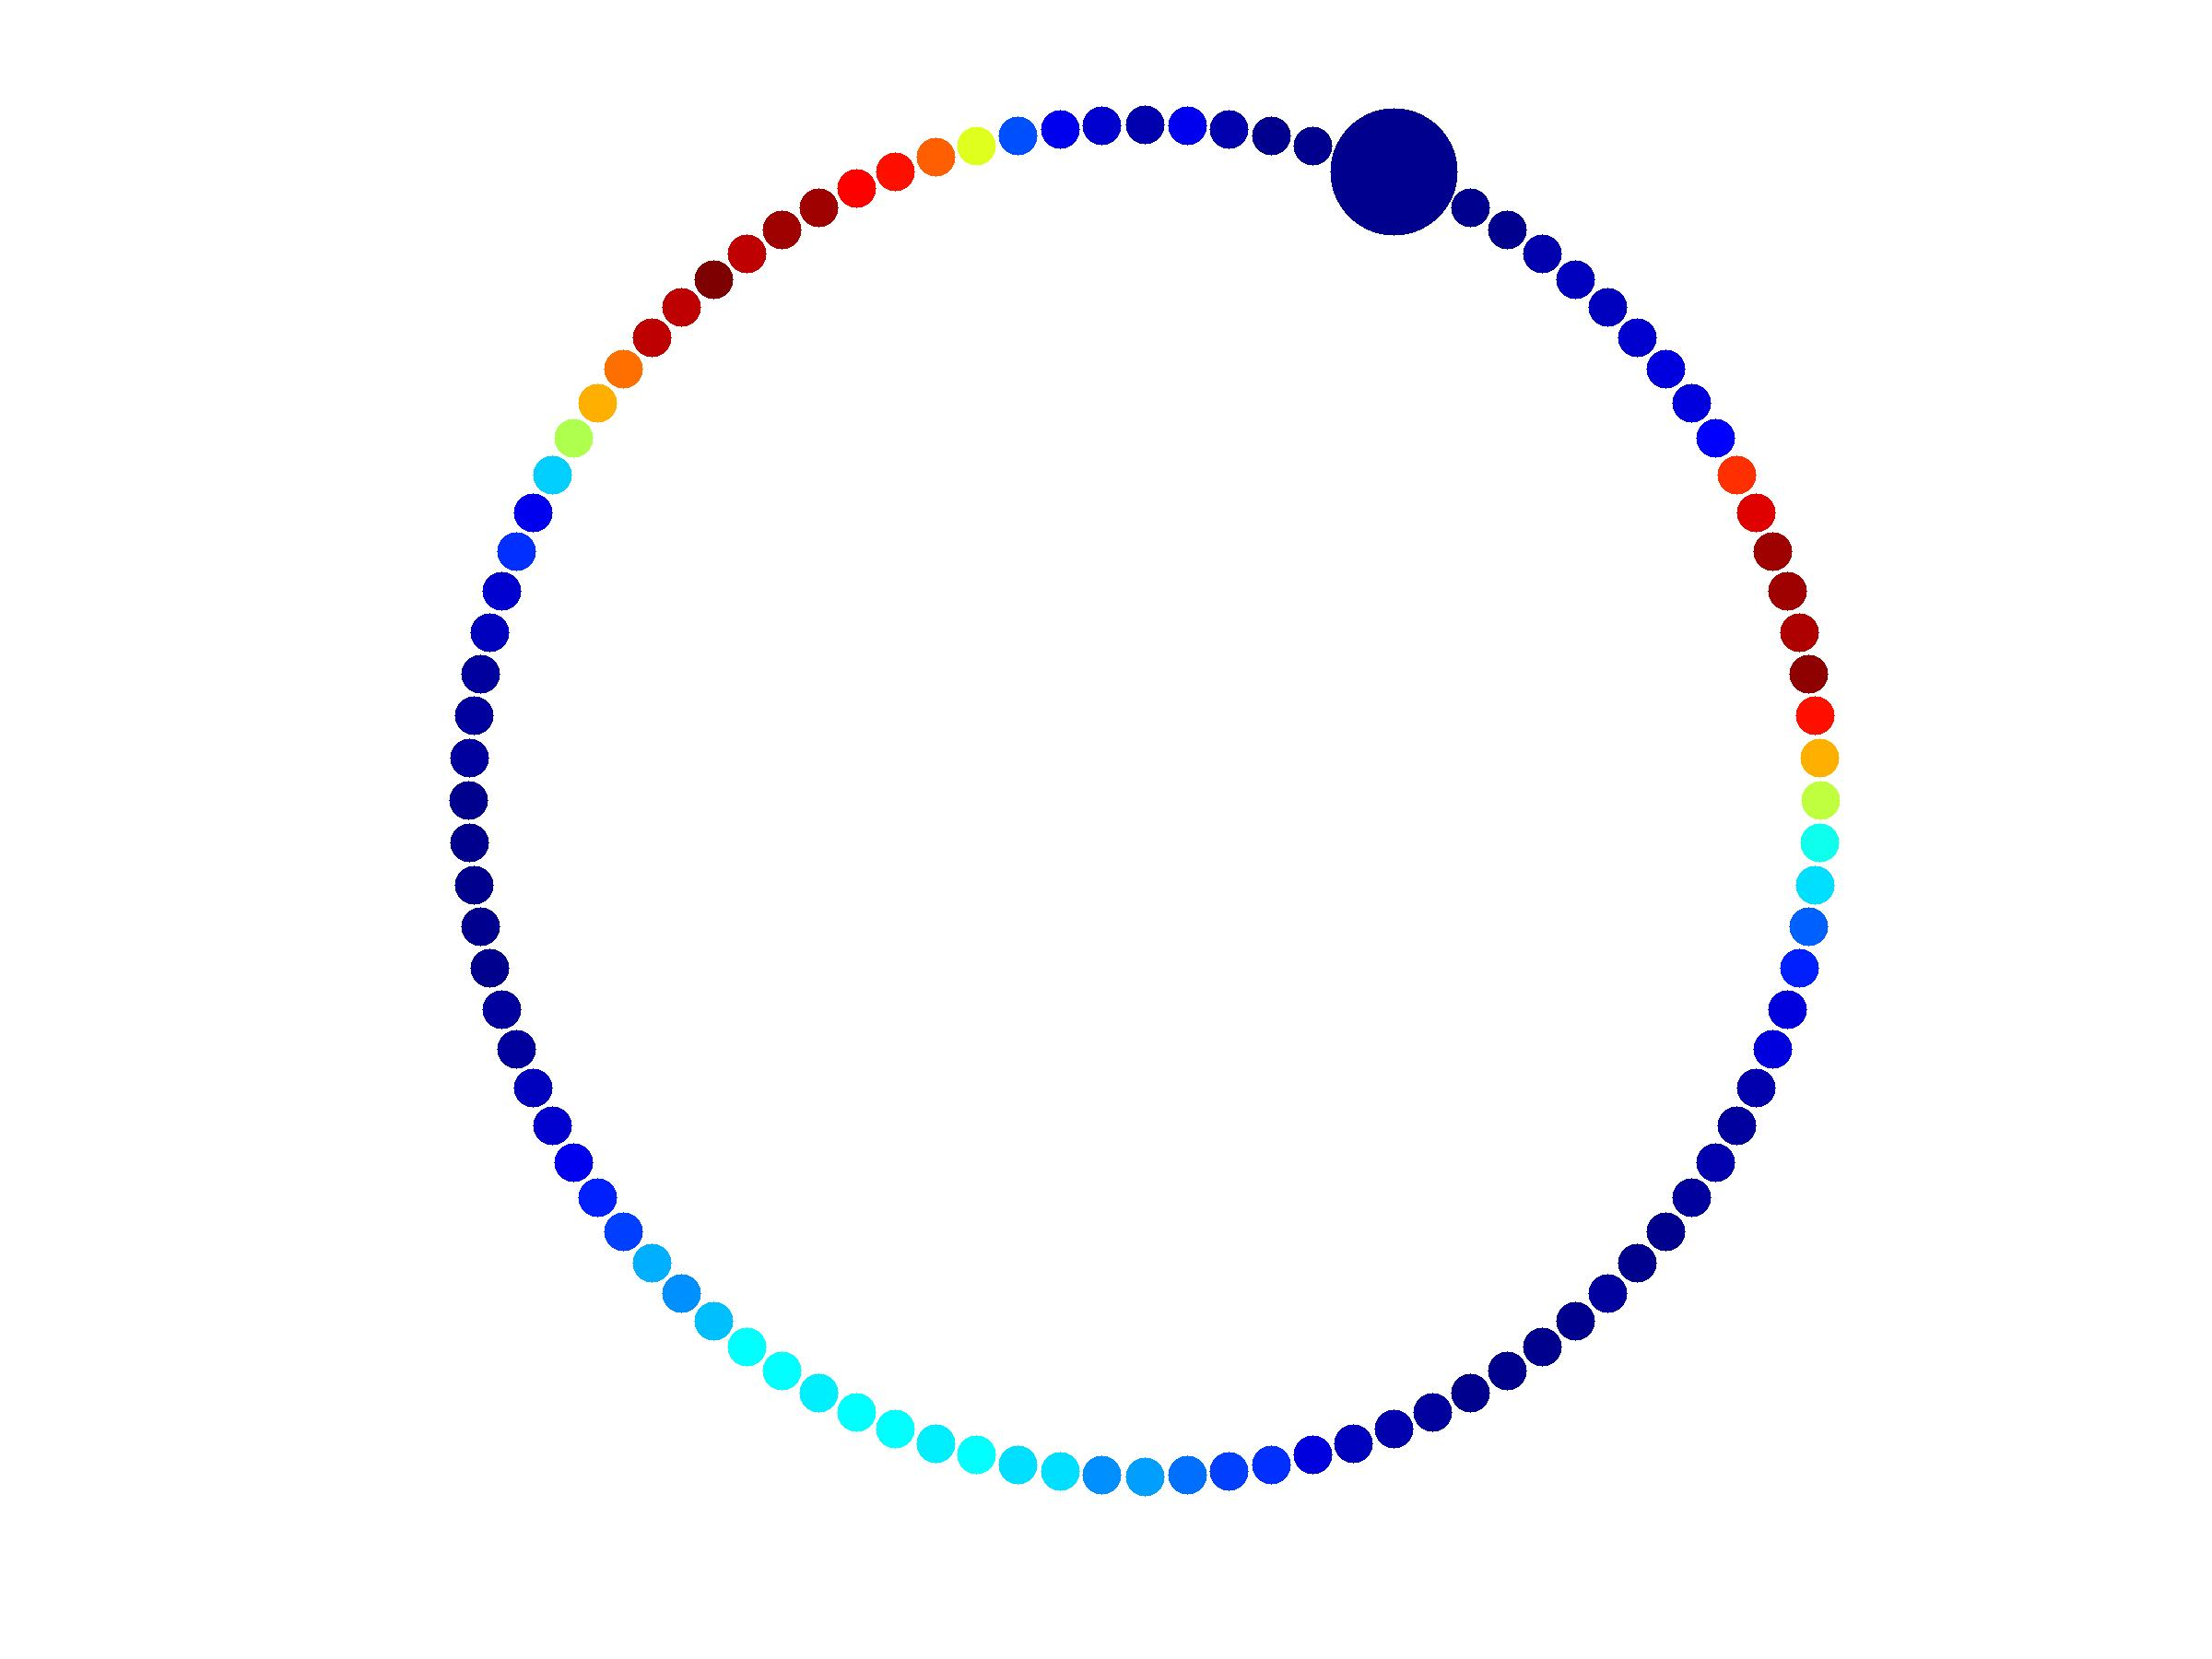
\includegraphics[width=0.45\textwidth]{../SIAM_DS_2013/drosophila_rot7.jpg}
            \end{minipage}};
            \draw [->] (fig1.east) -- (fig2.west);
        \end{tikzpicture}
        {\scriptsize \em This results in sines and cosines as PCA modes \footnotemark \par}
	\end{block}
	
	\footcitetext{sirovich1987turbulence}
	
	\vspace{-0.3in}
	
	\begin{block}{}
        \begin{tikzpicture}
        	\node [text width=0.3\textwidth] (text1) {{\bf We can use rotations to {\em reduce} data} \\ We first align the data before doing further analysis};
            \node[right=of text1] (fig1) {
            \begin{minipage}{0.25\textwidth}
            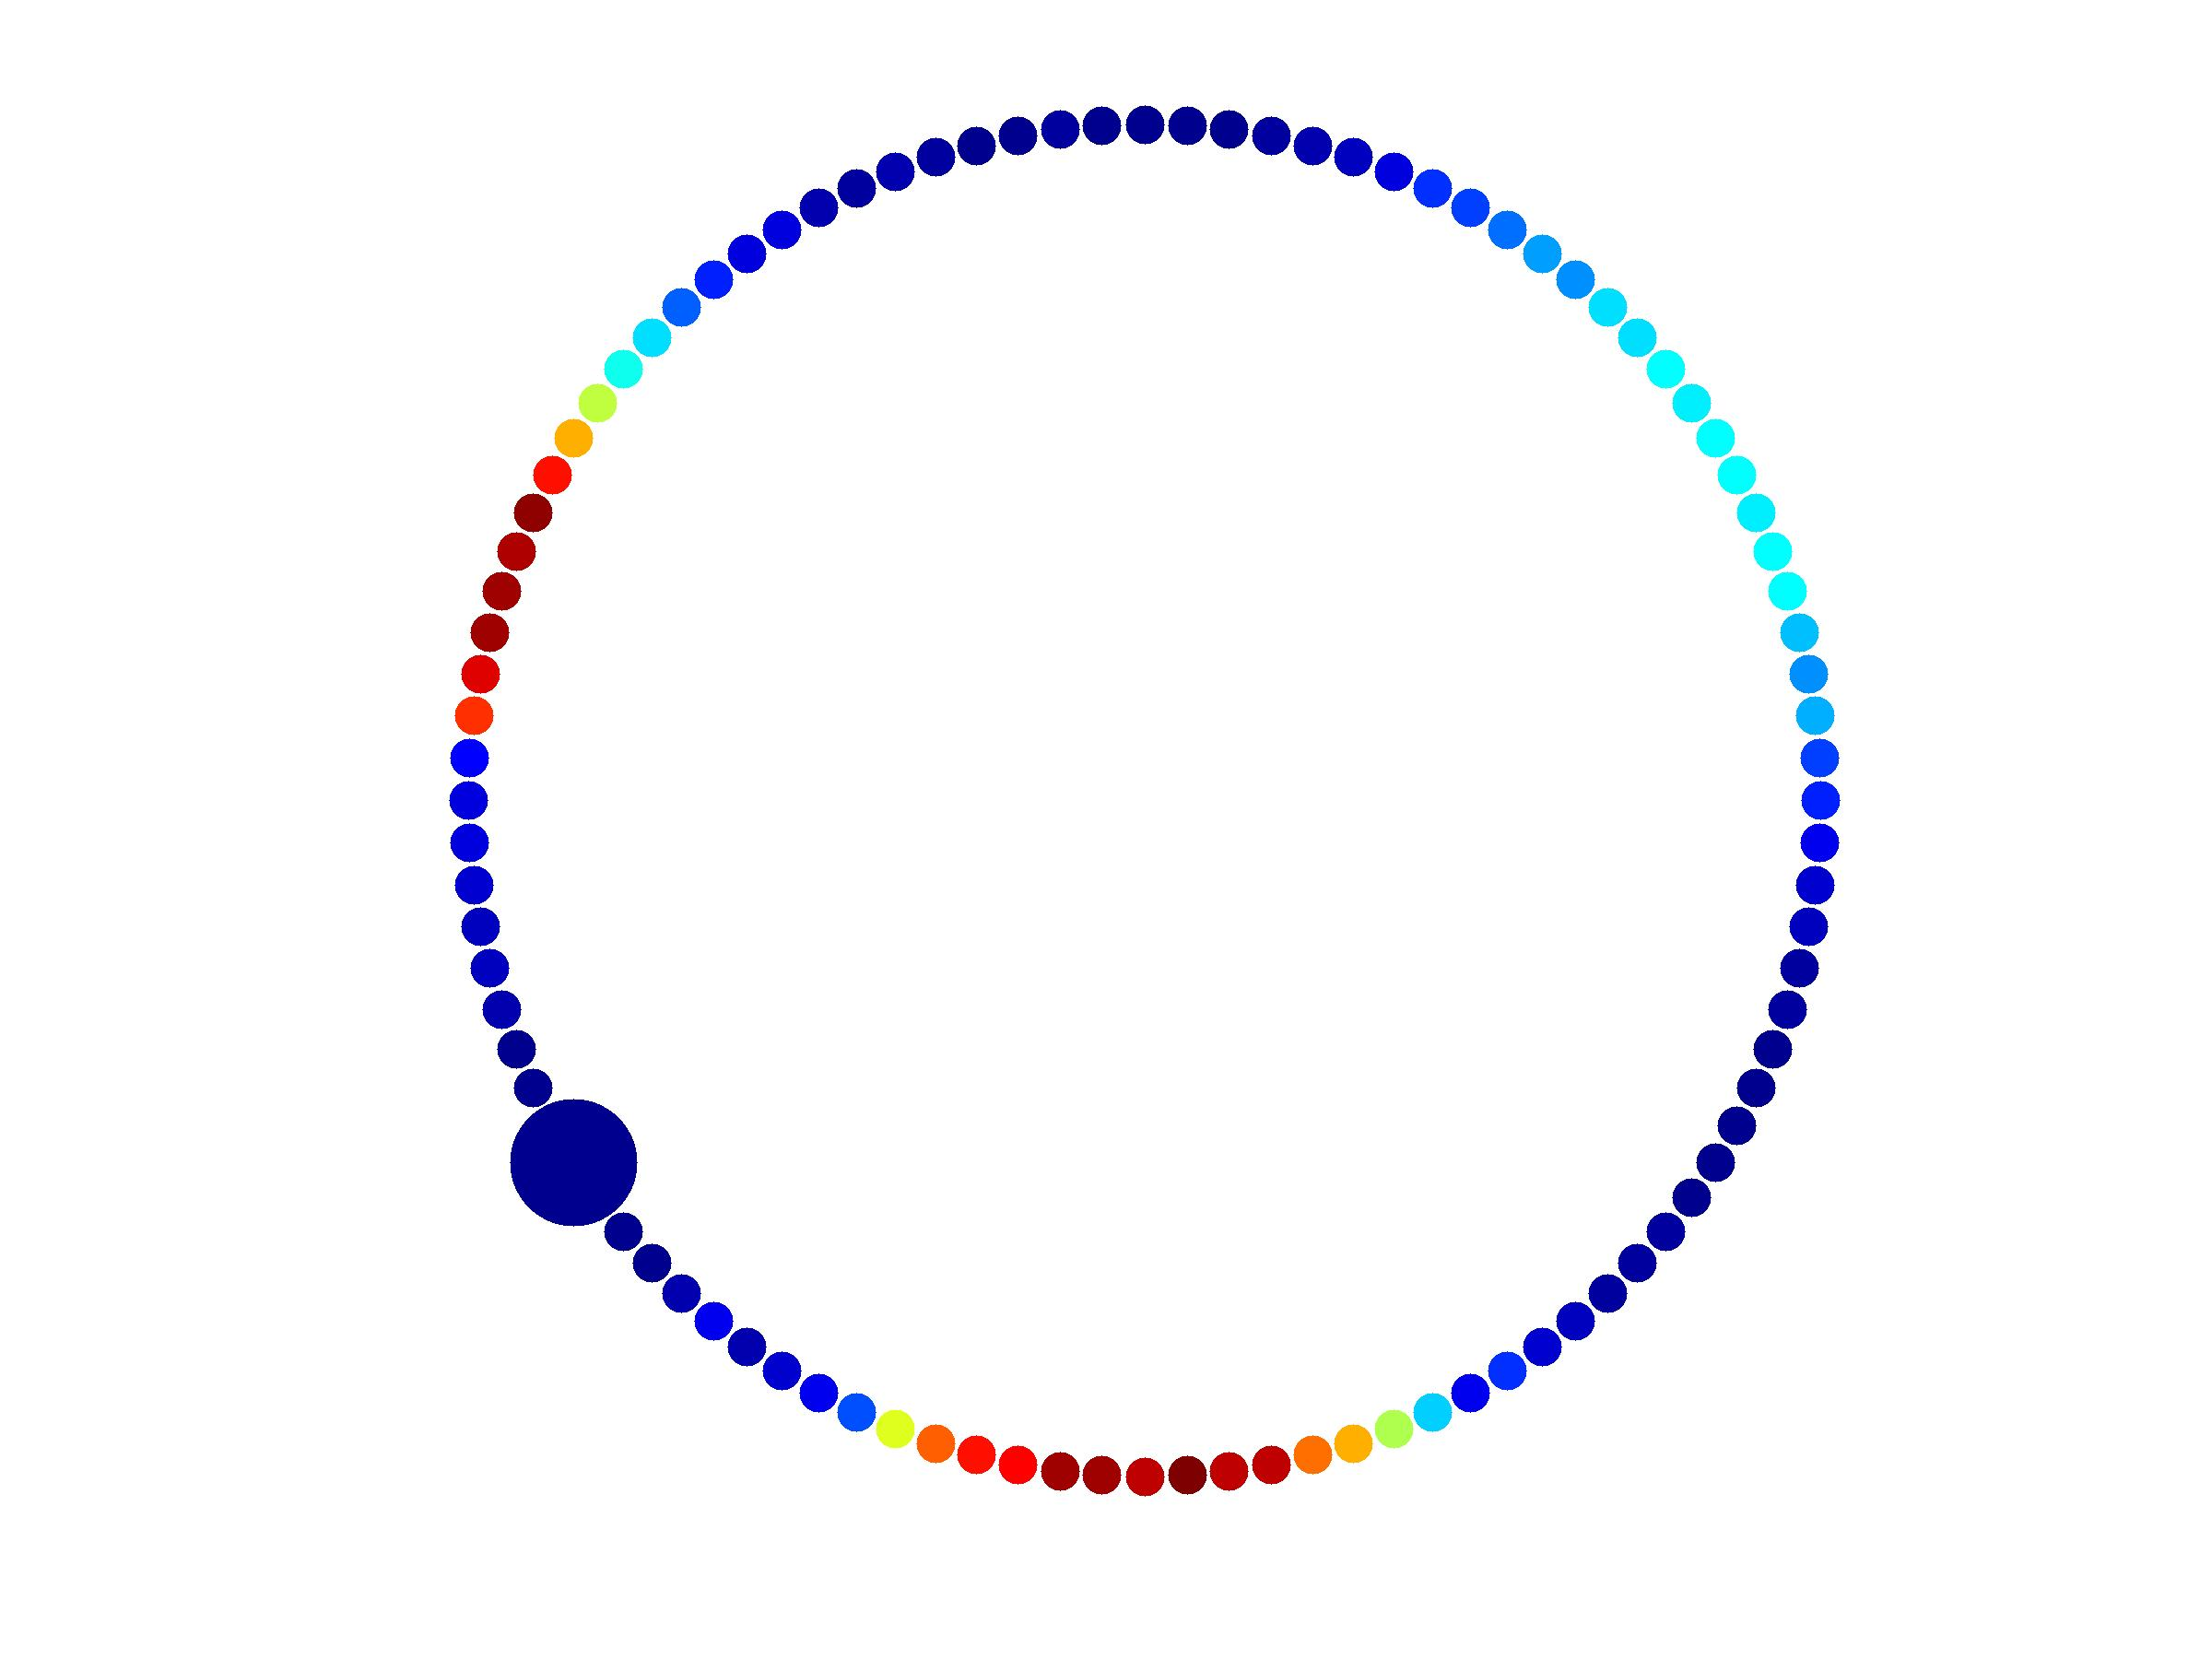
\includegraphics[width=0.45\textwidth]{../SIAM_DS_2013/drosophila_rot1.jpg}
            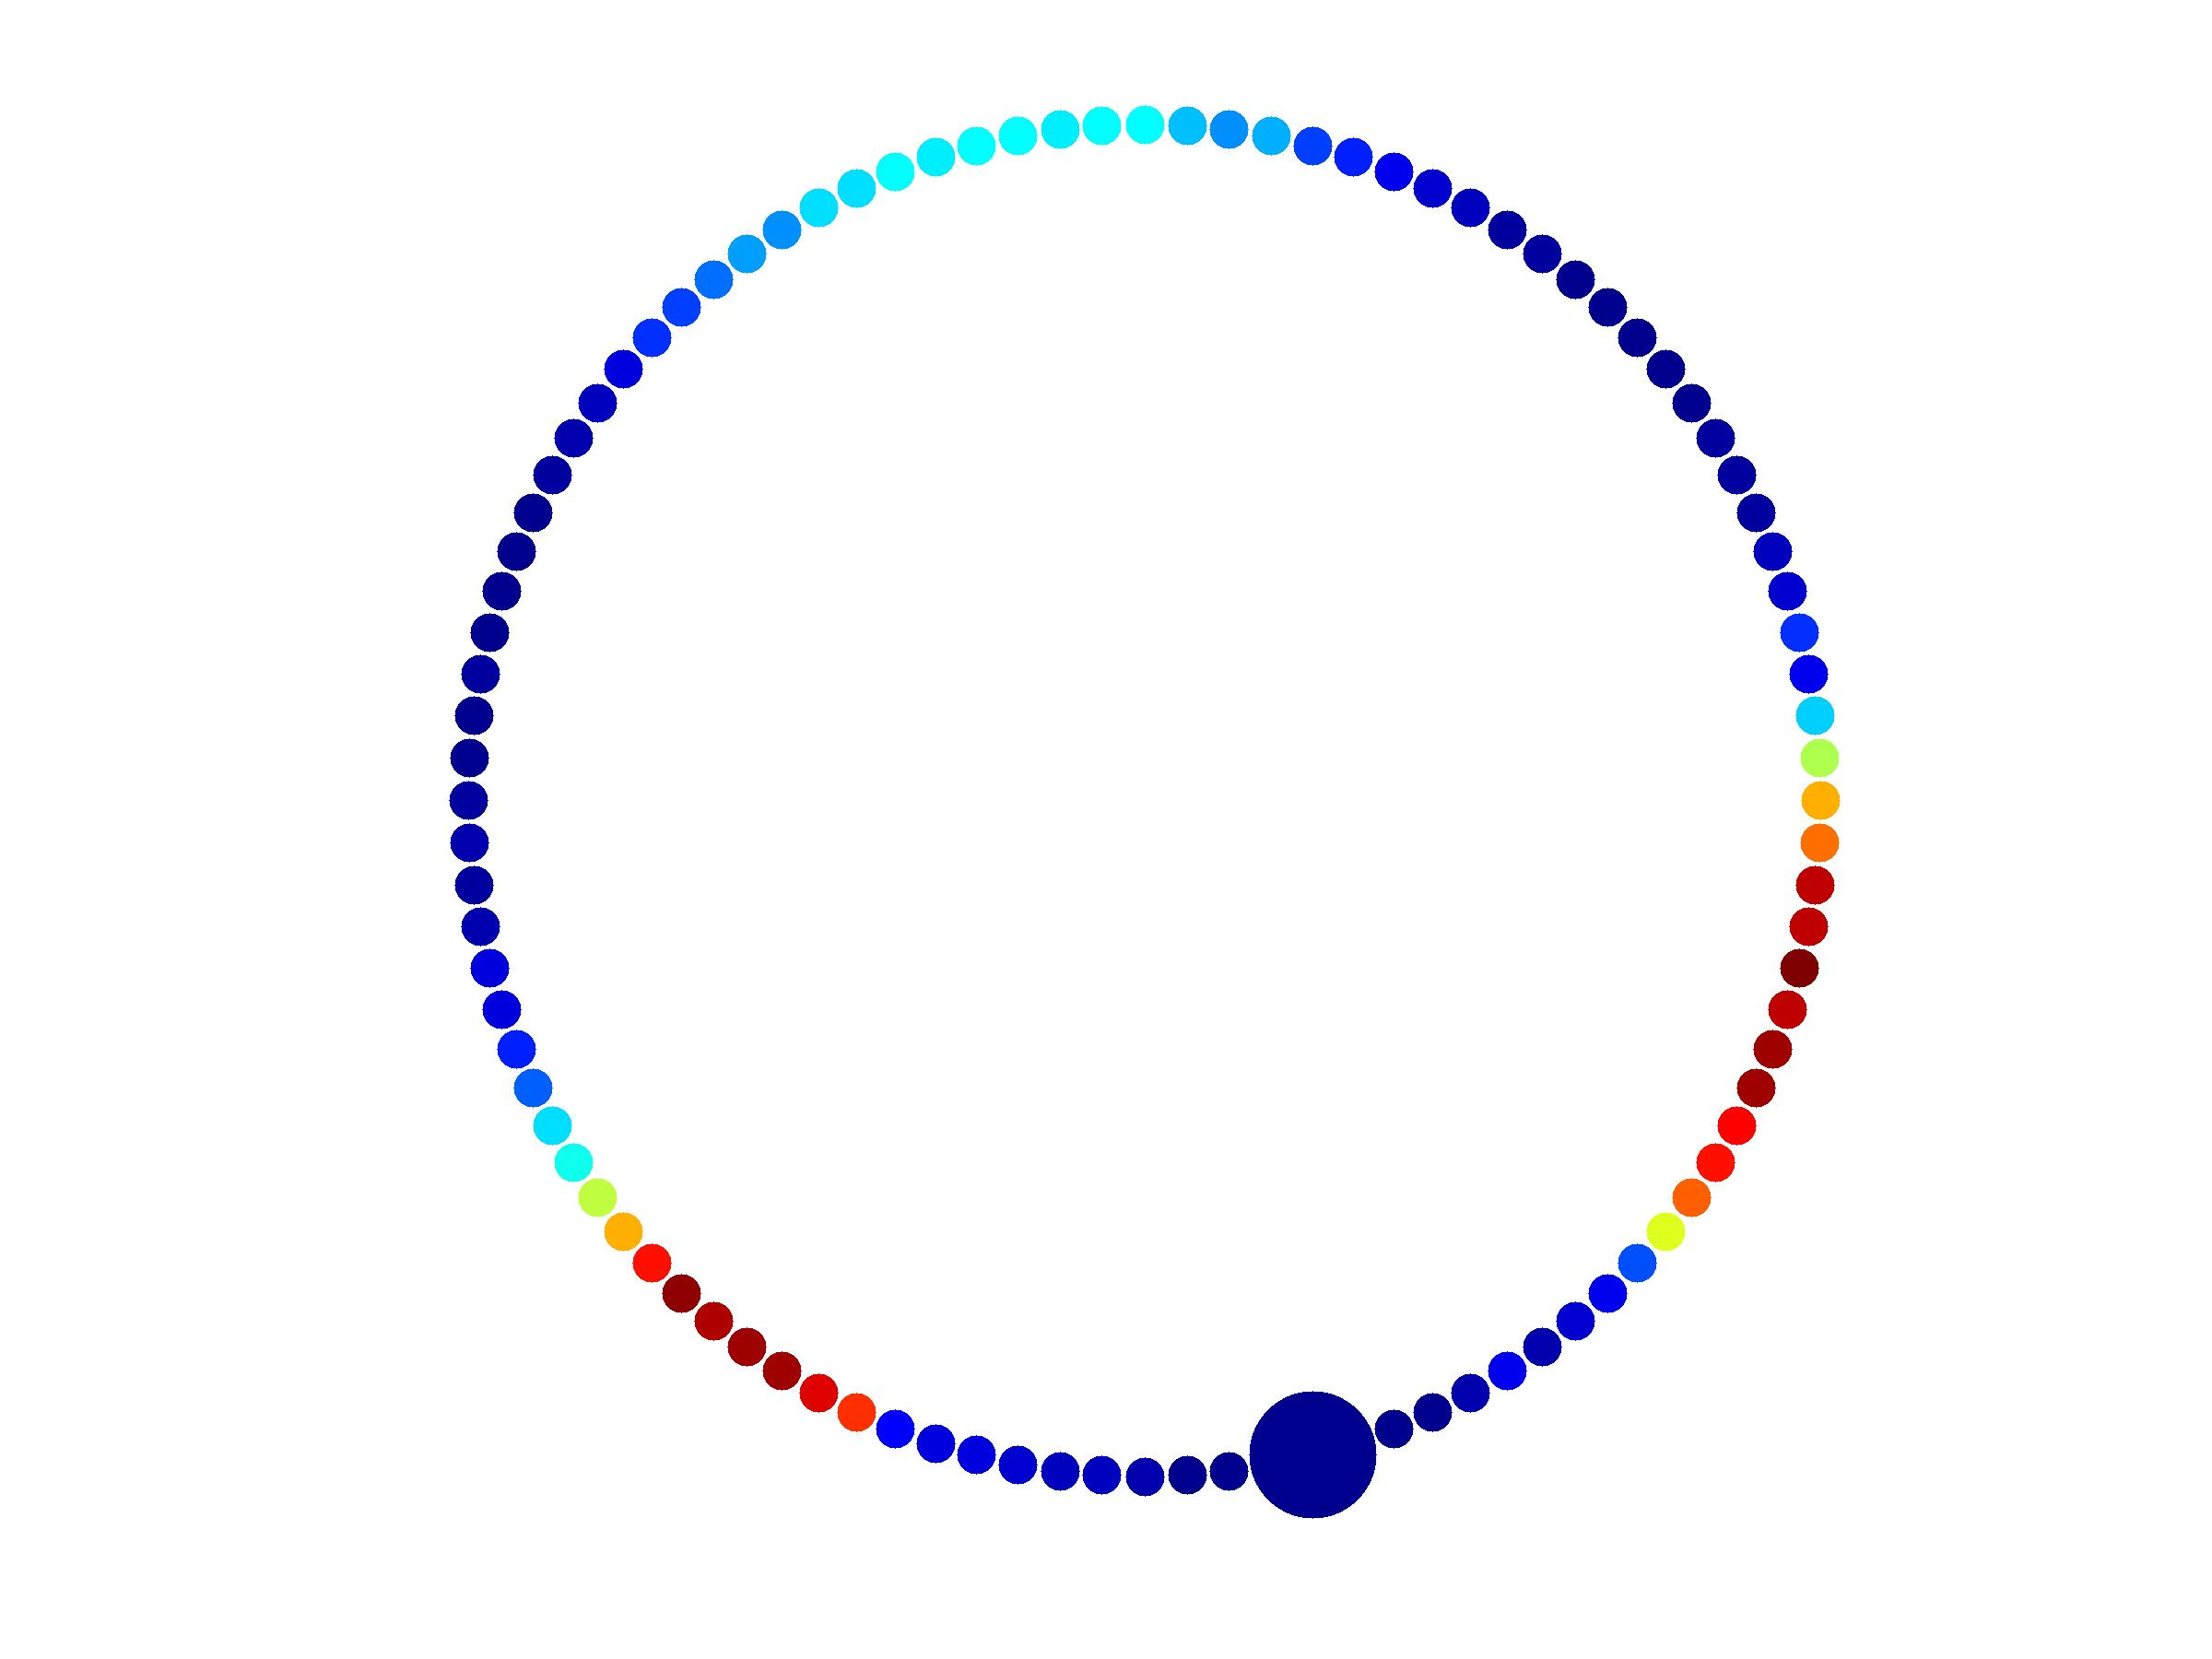
\includegraphics[width=0.45\textwidth]{../SIAM_DS_2013/drosophila_rot3.jpg}\\
			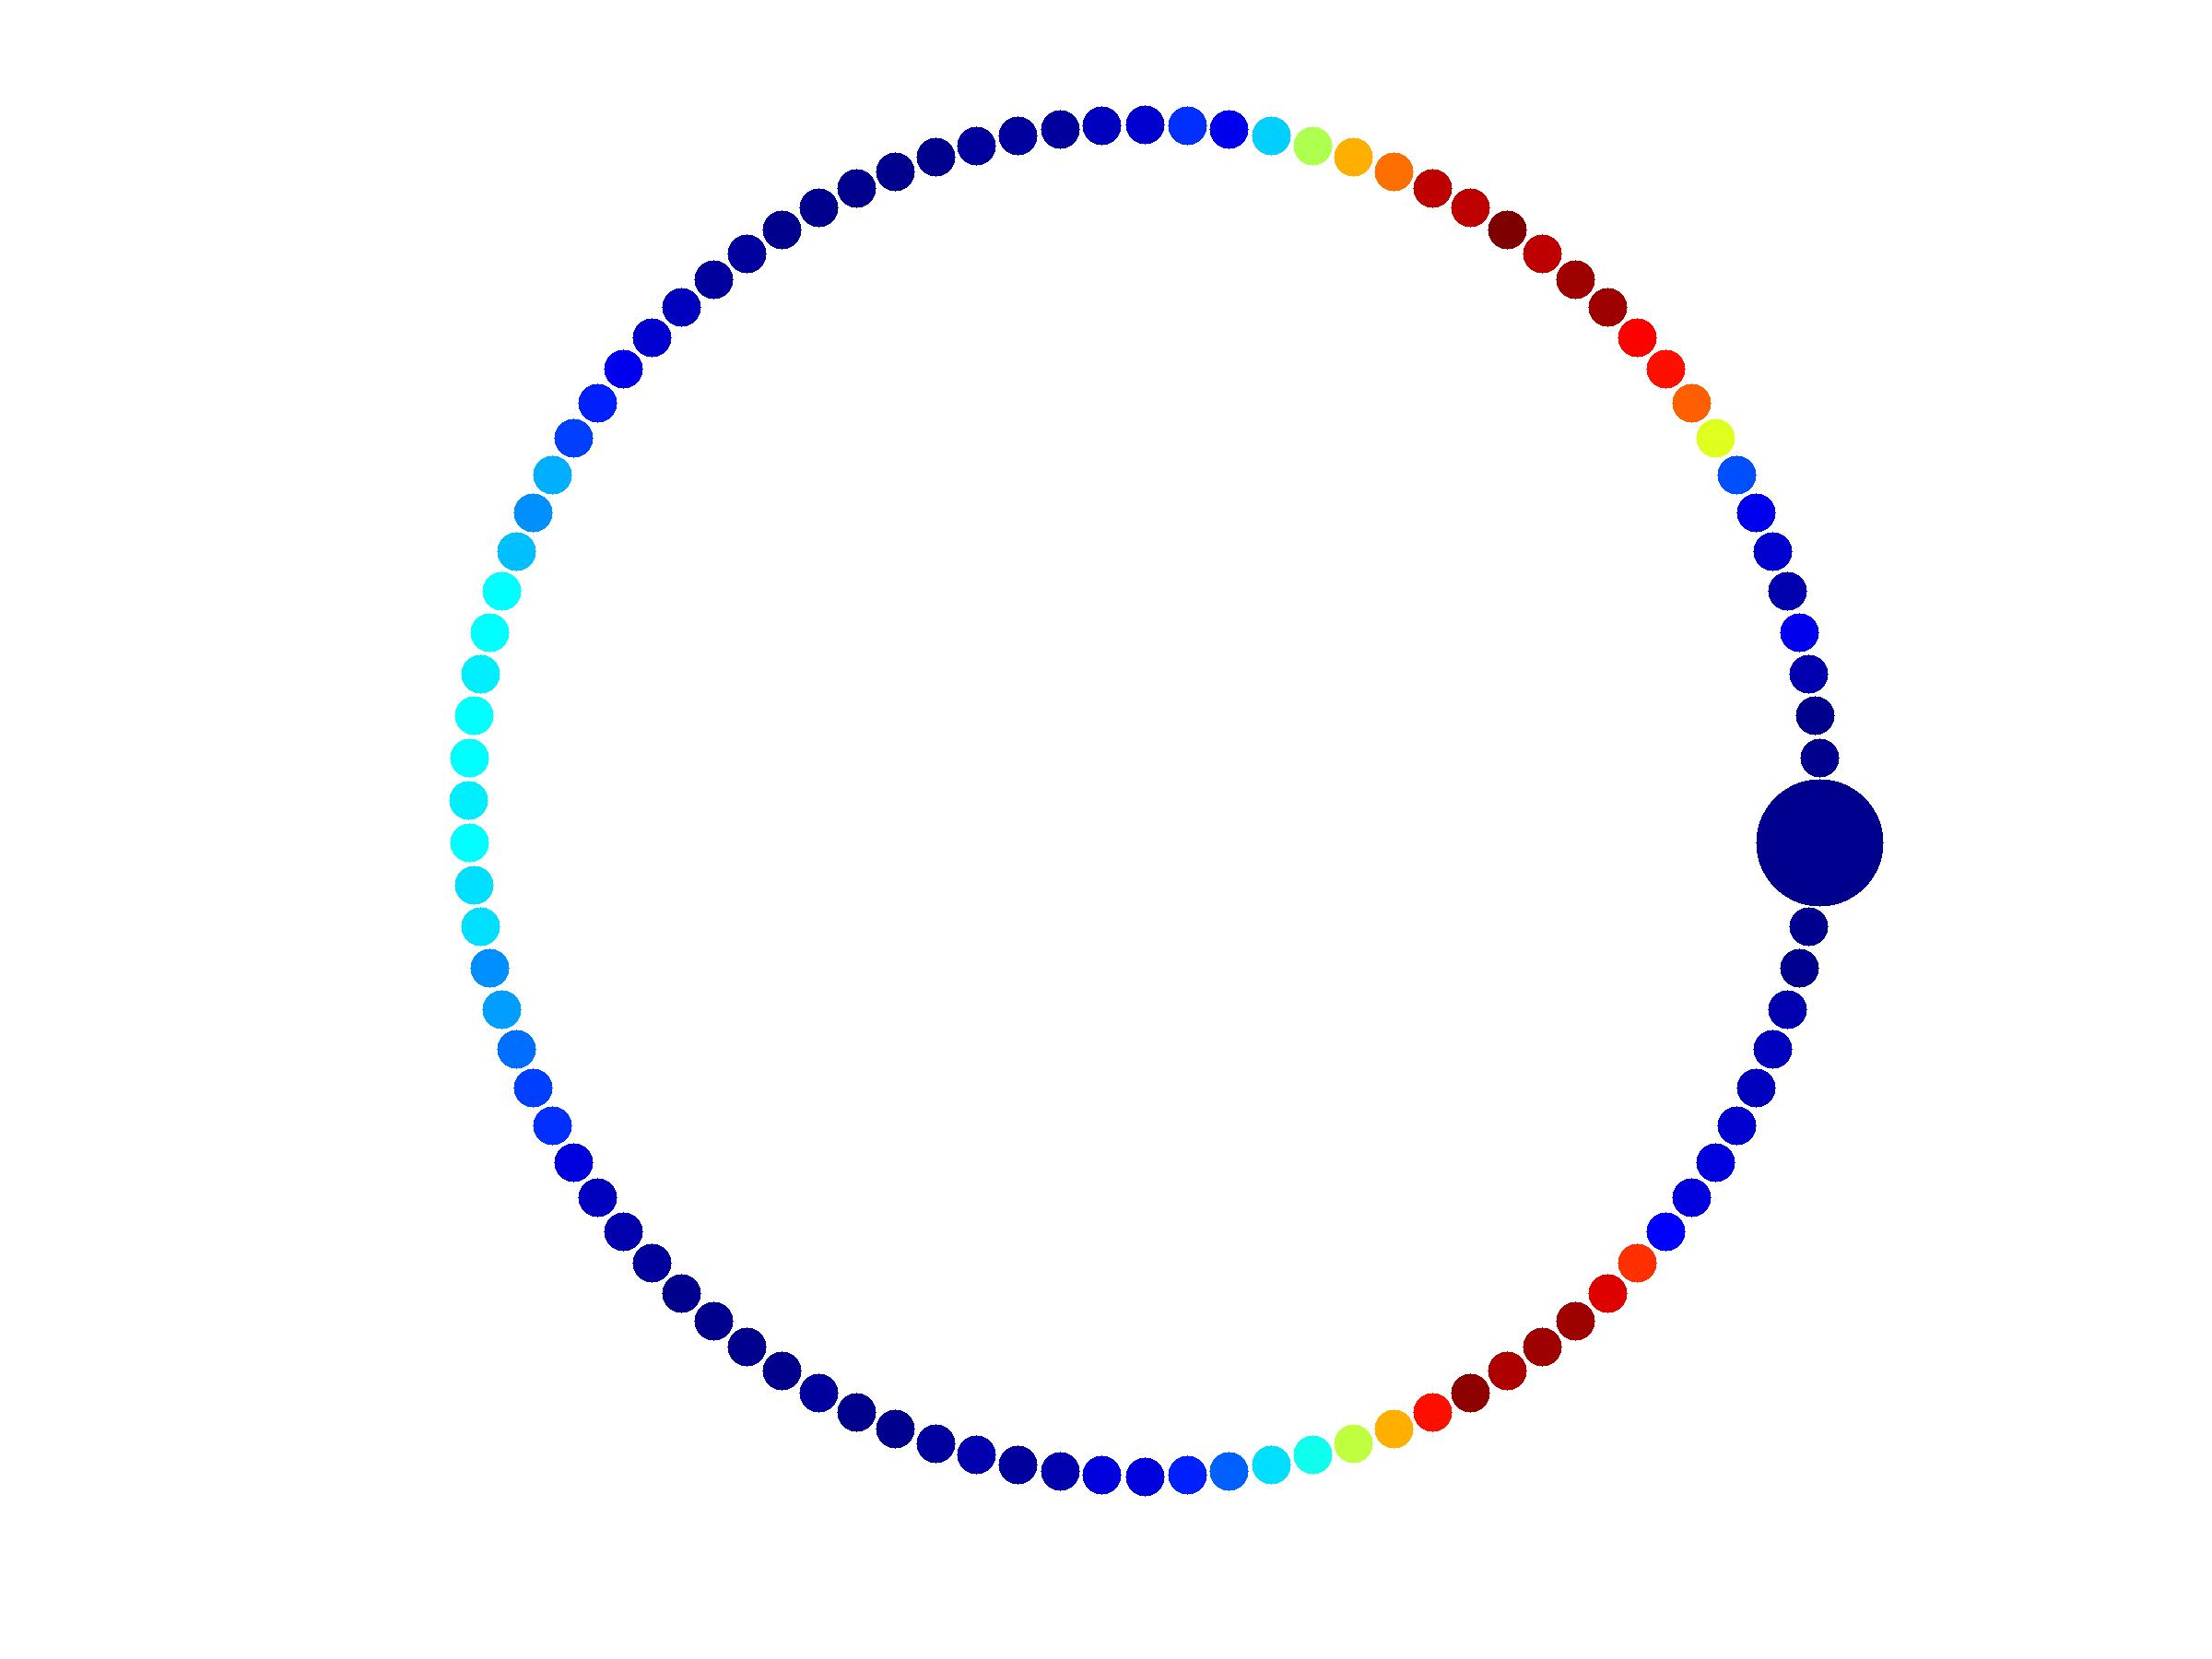
\includegraphics[width=0.45\textwidth]{../SIAM_DS_2013/drosophila_rot5.jpg}
            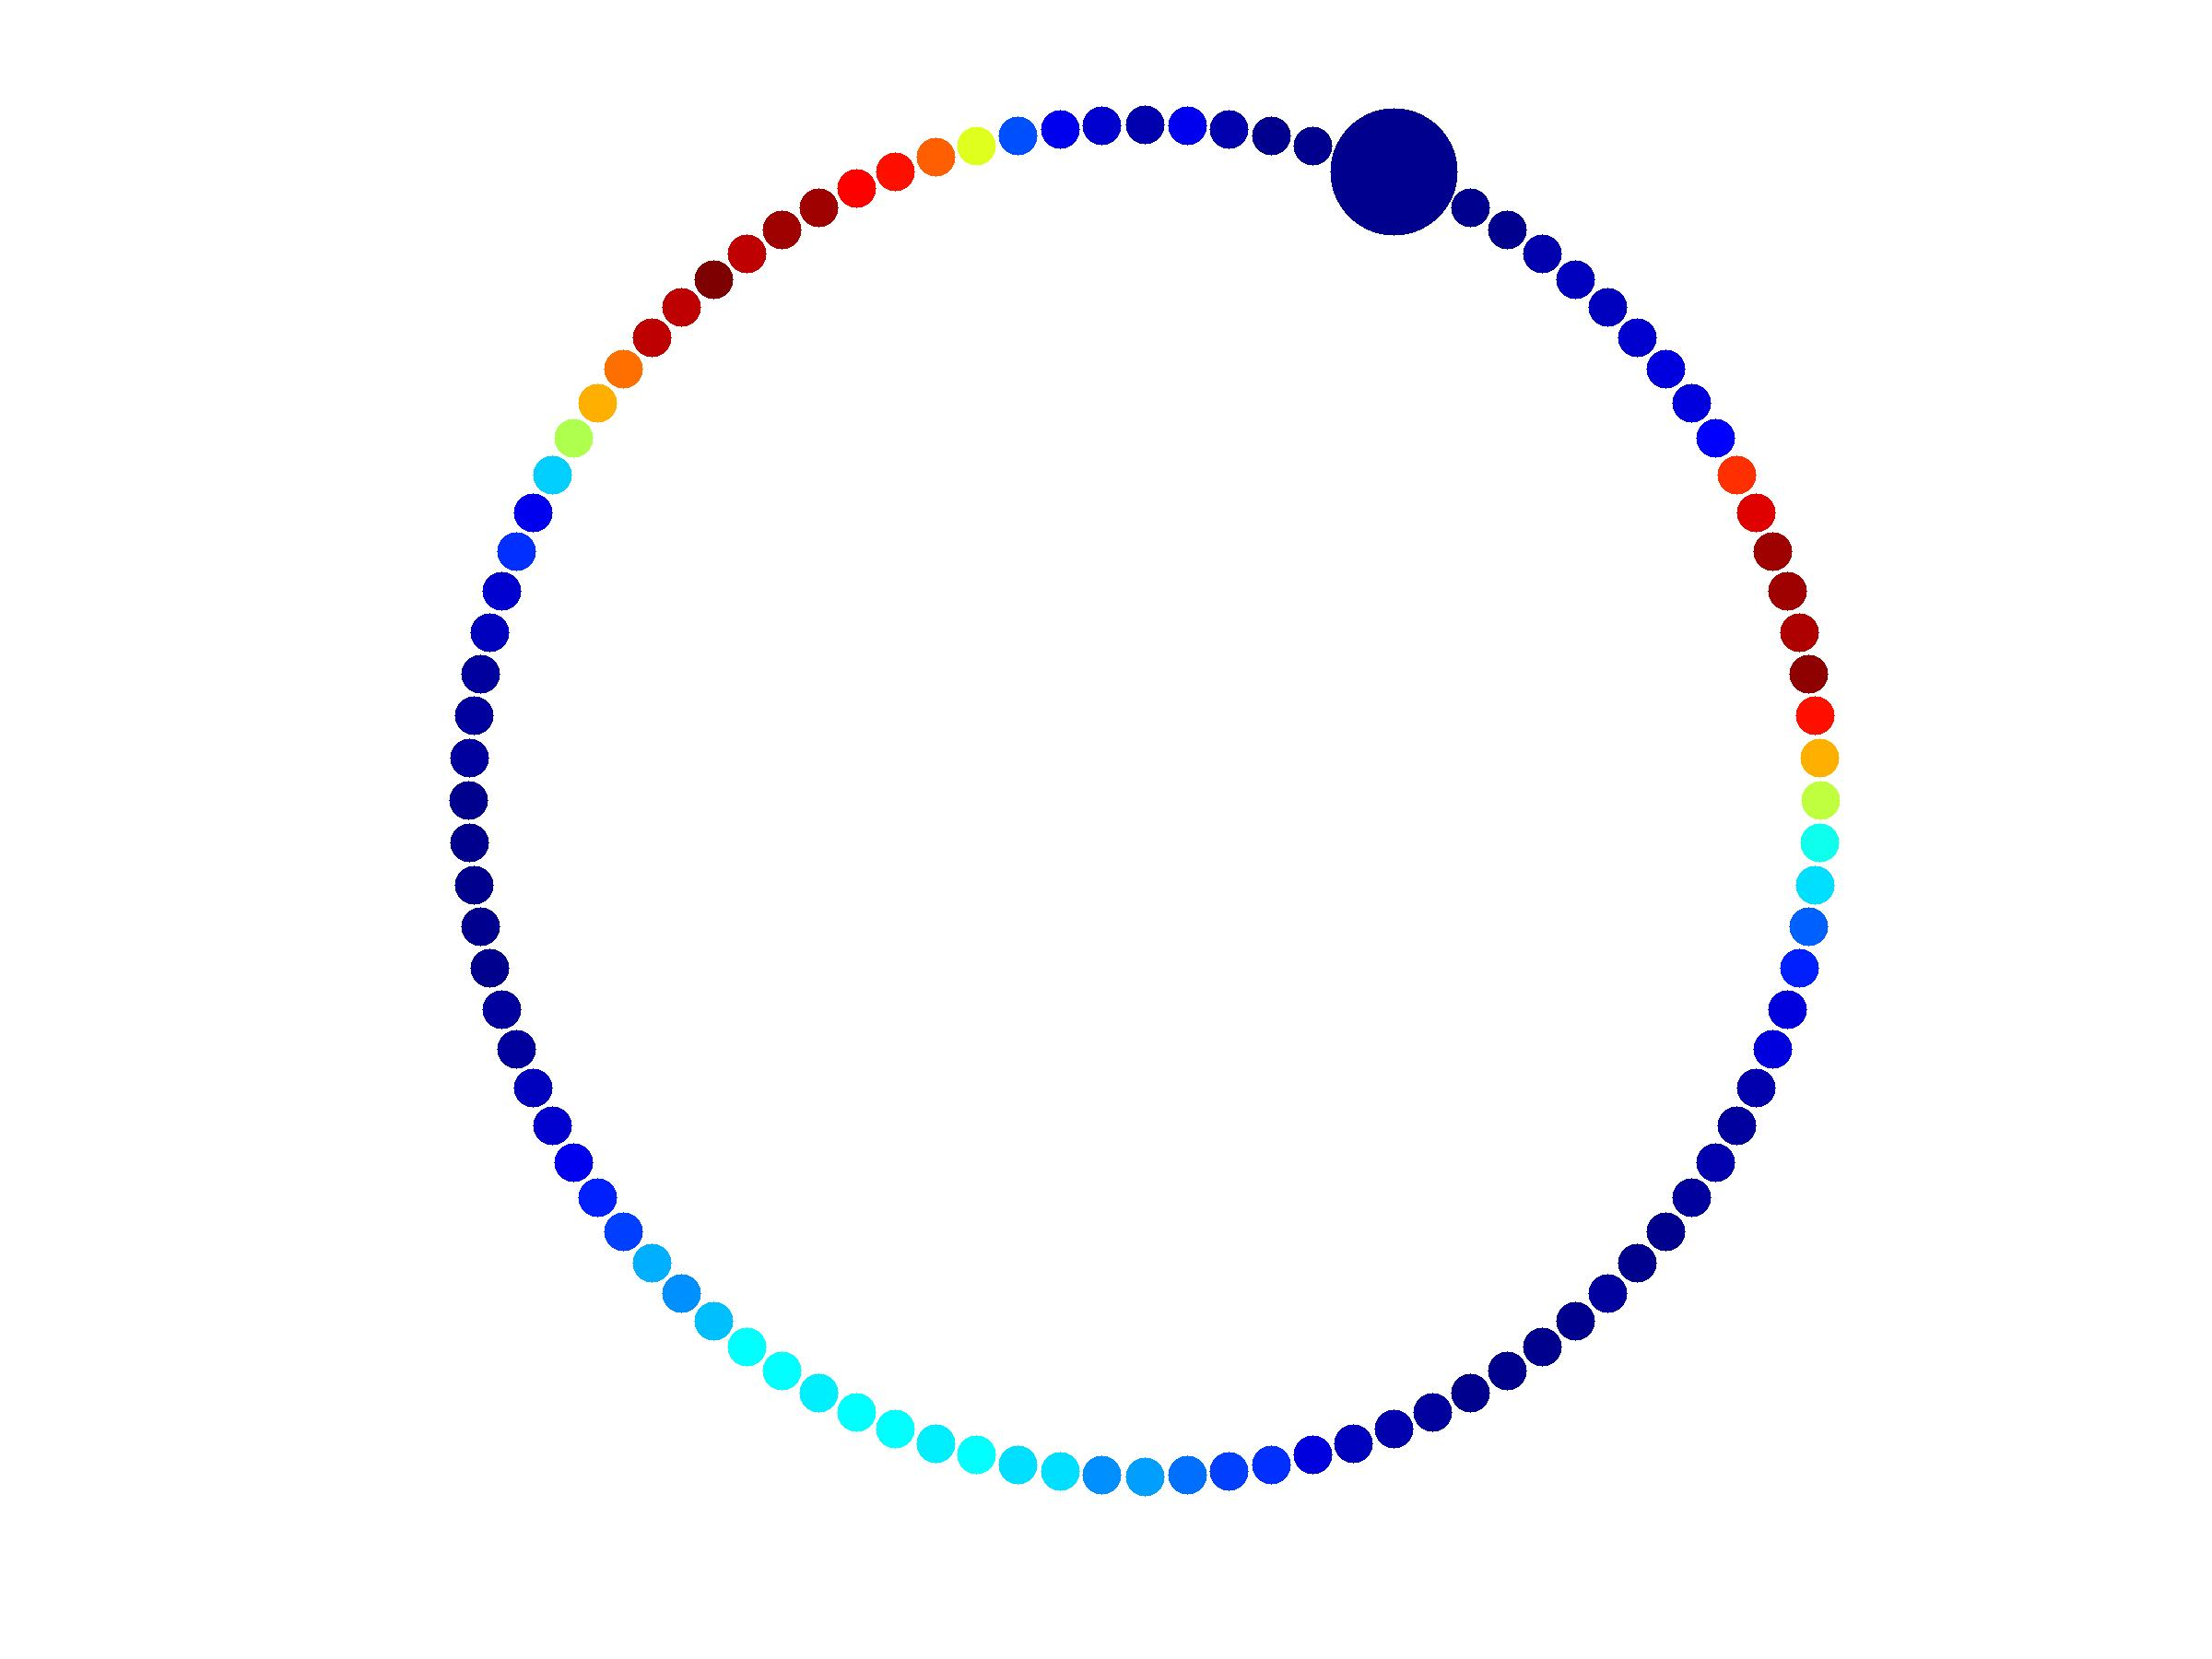
\includegraphics[width=0.45\textwidth]{../SIAM_DS_2013/drosophila_rot7.jpg}
            \end{minipage}};
            
            \node [right of=fig1, node distance=0.35\textwidth] (fig2) {
            \begin{minipage}{0.25\textwidth}
            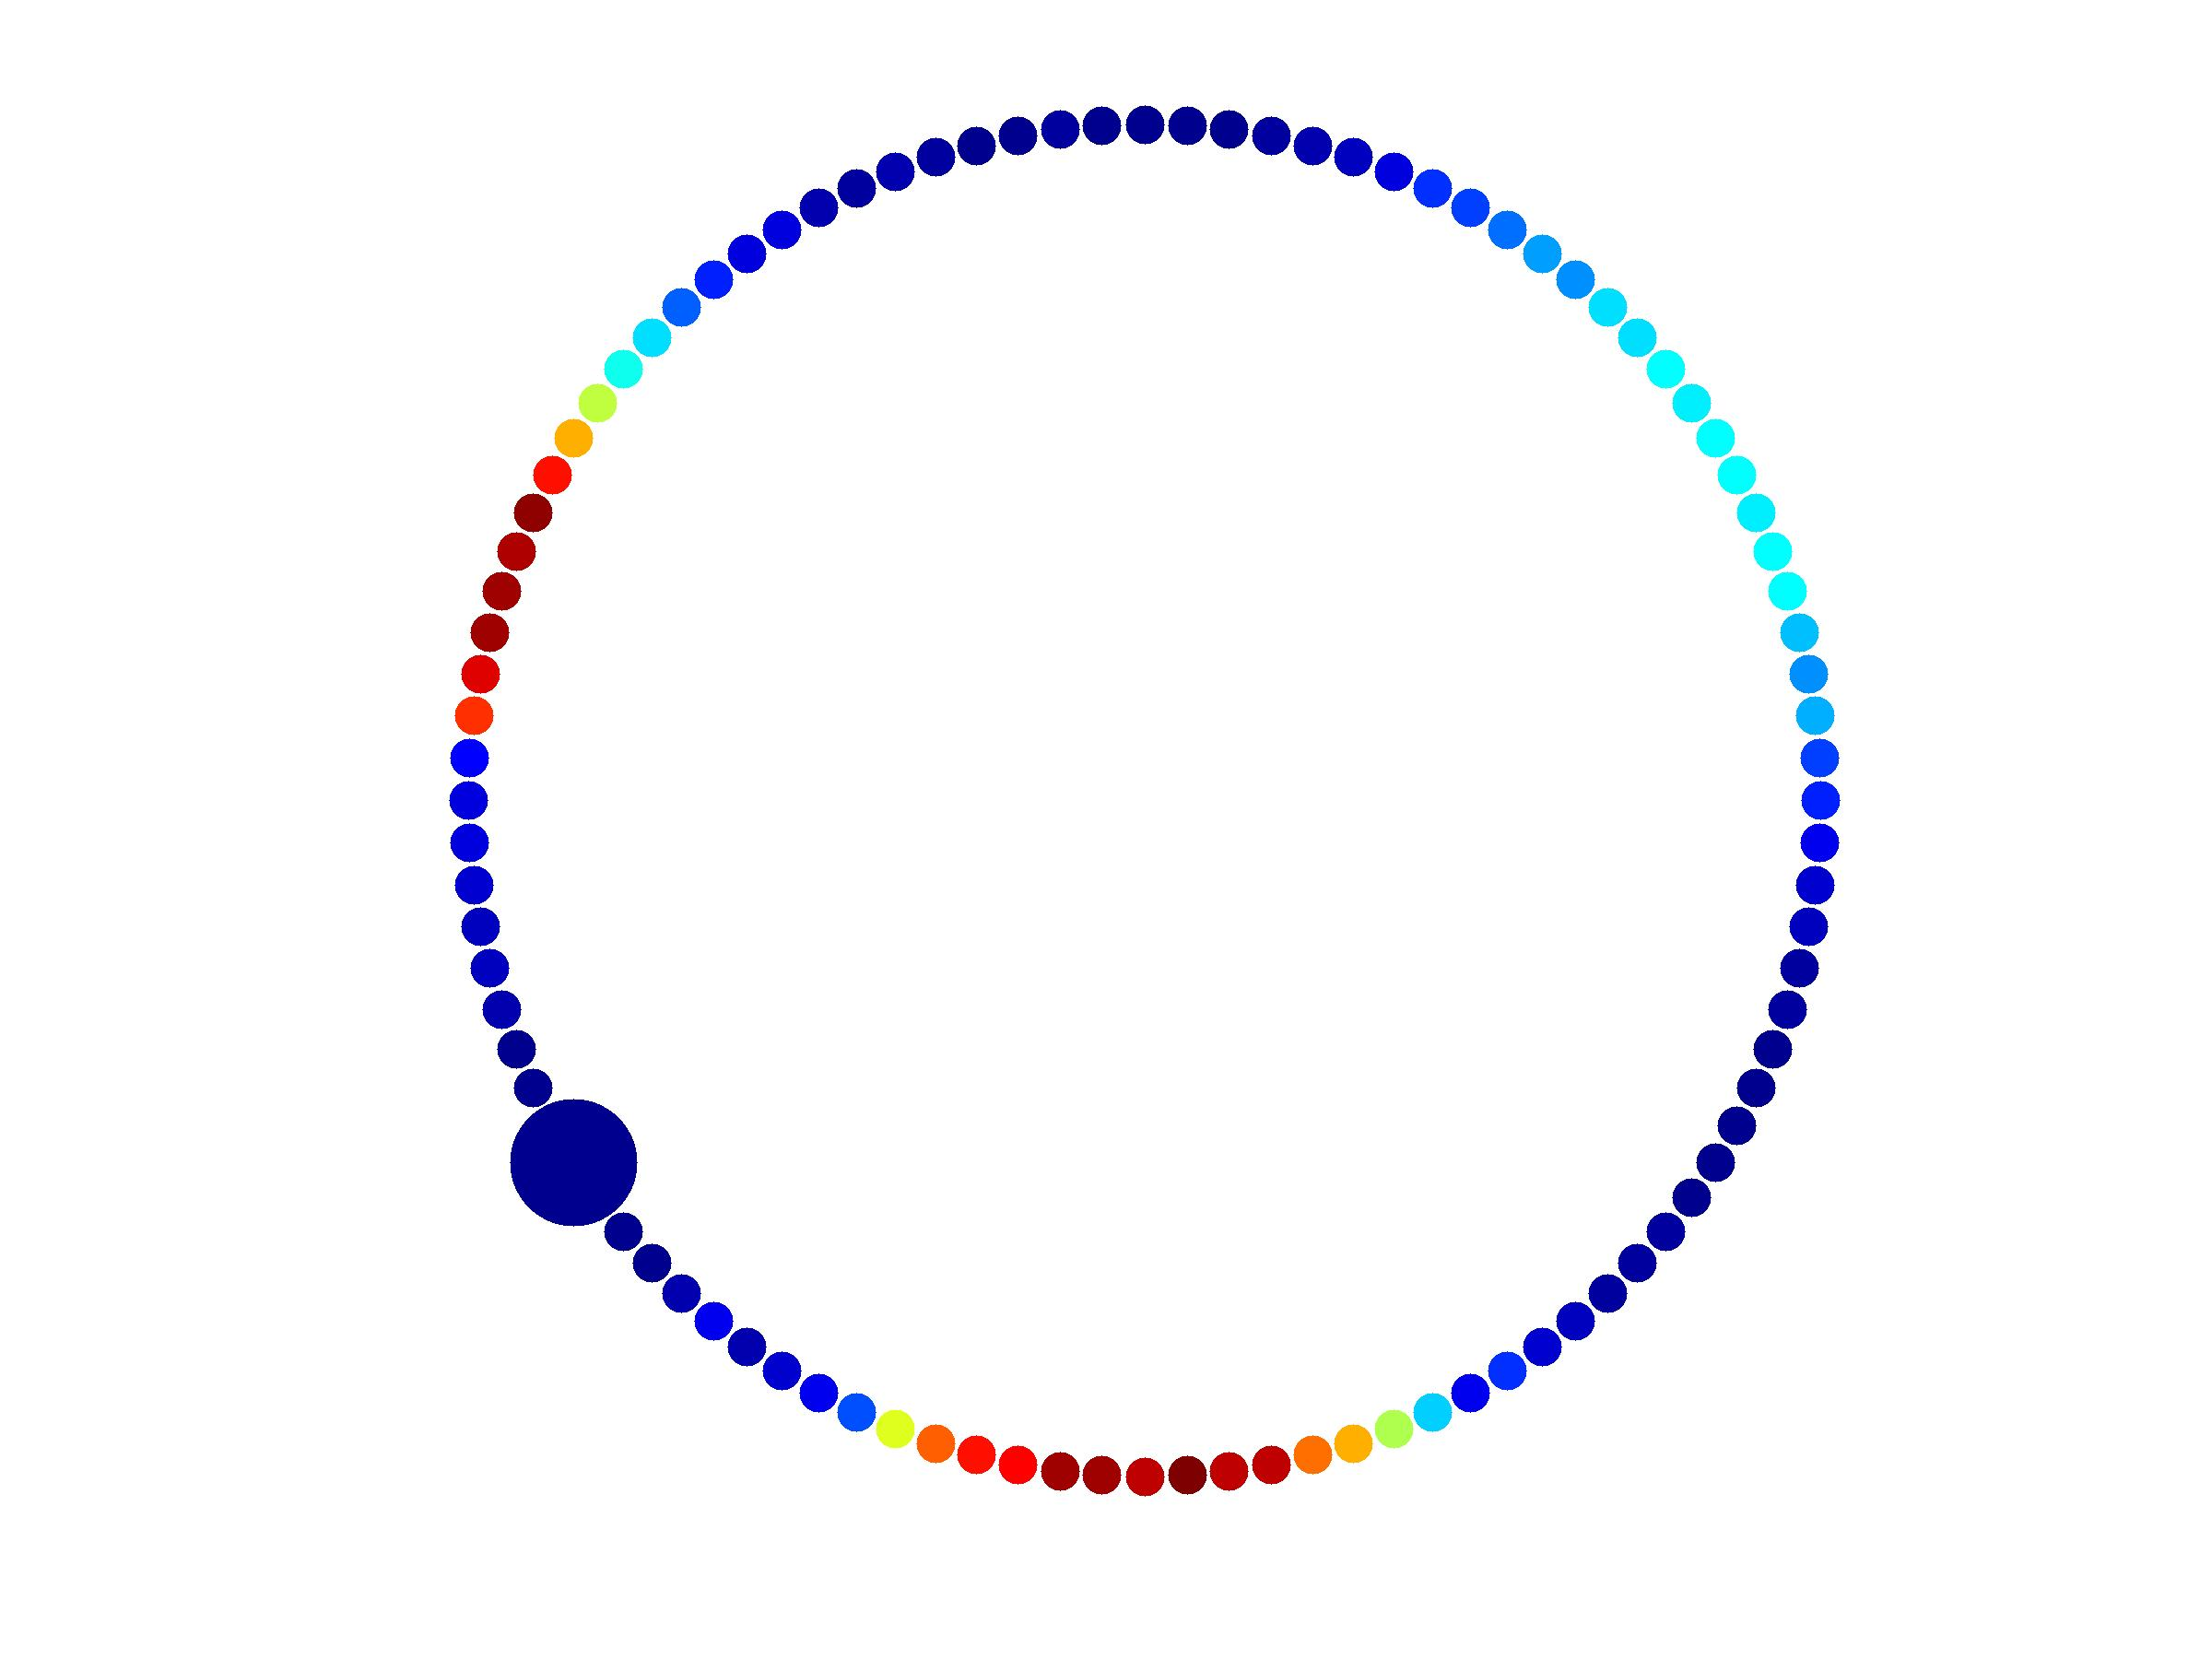
\includegraphics[width=0.45\textwidth]{../SIAM_DS_2013/drosophila_rot1.jpg}
            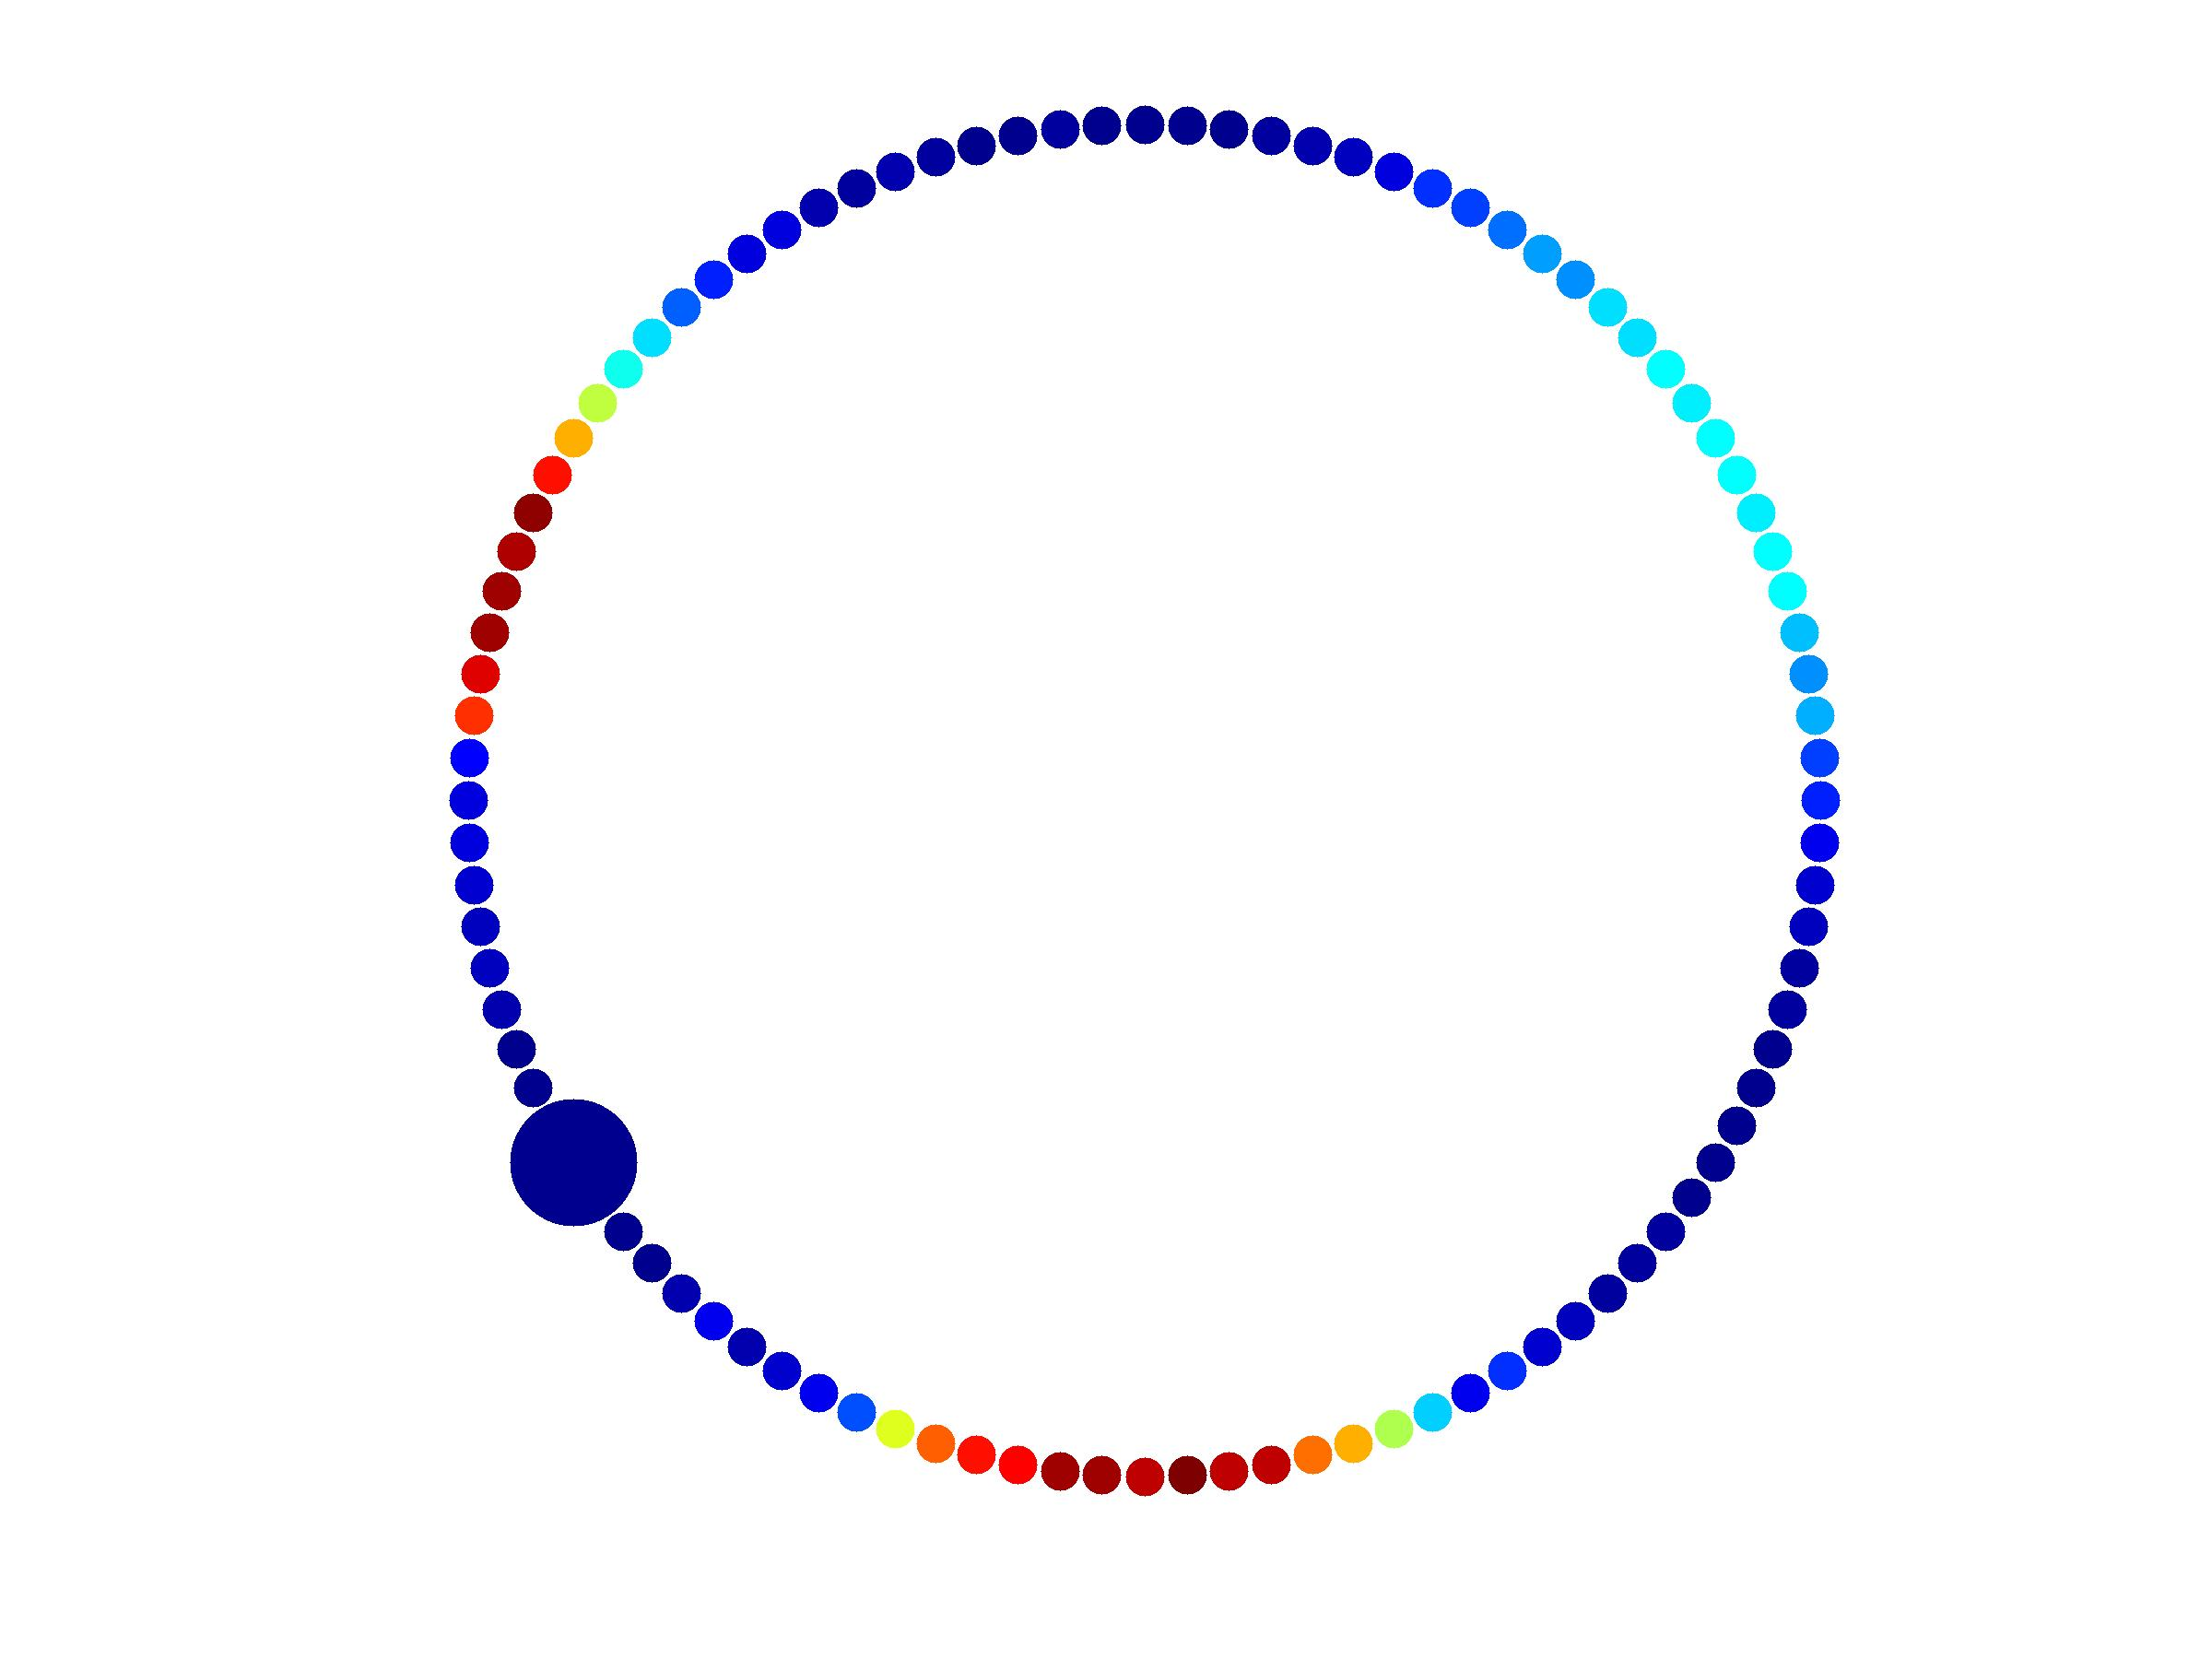
\includegraphics[width=0.45\textwidth]{../SIAM_DS_2013/drosophila_rot1.jpg}\\
            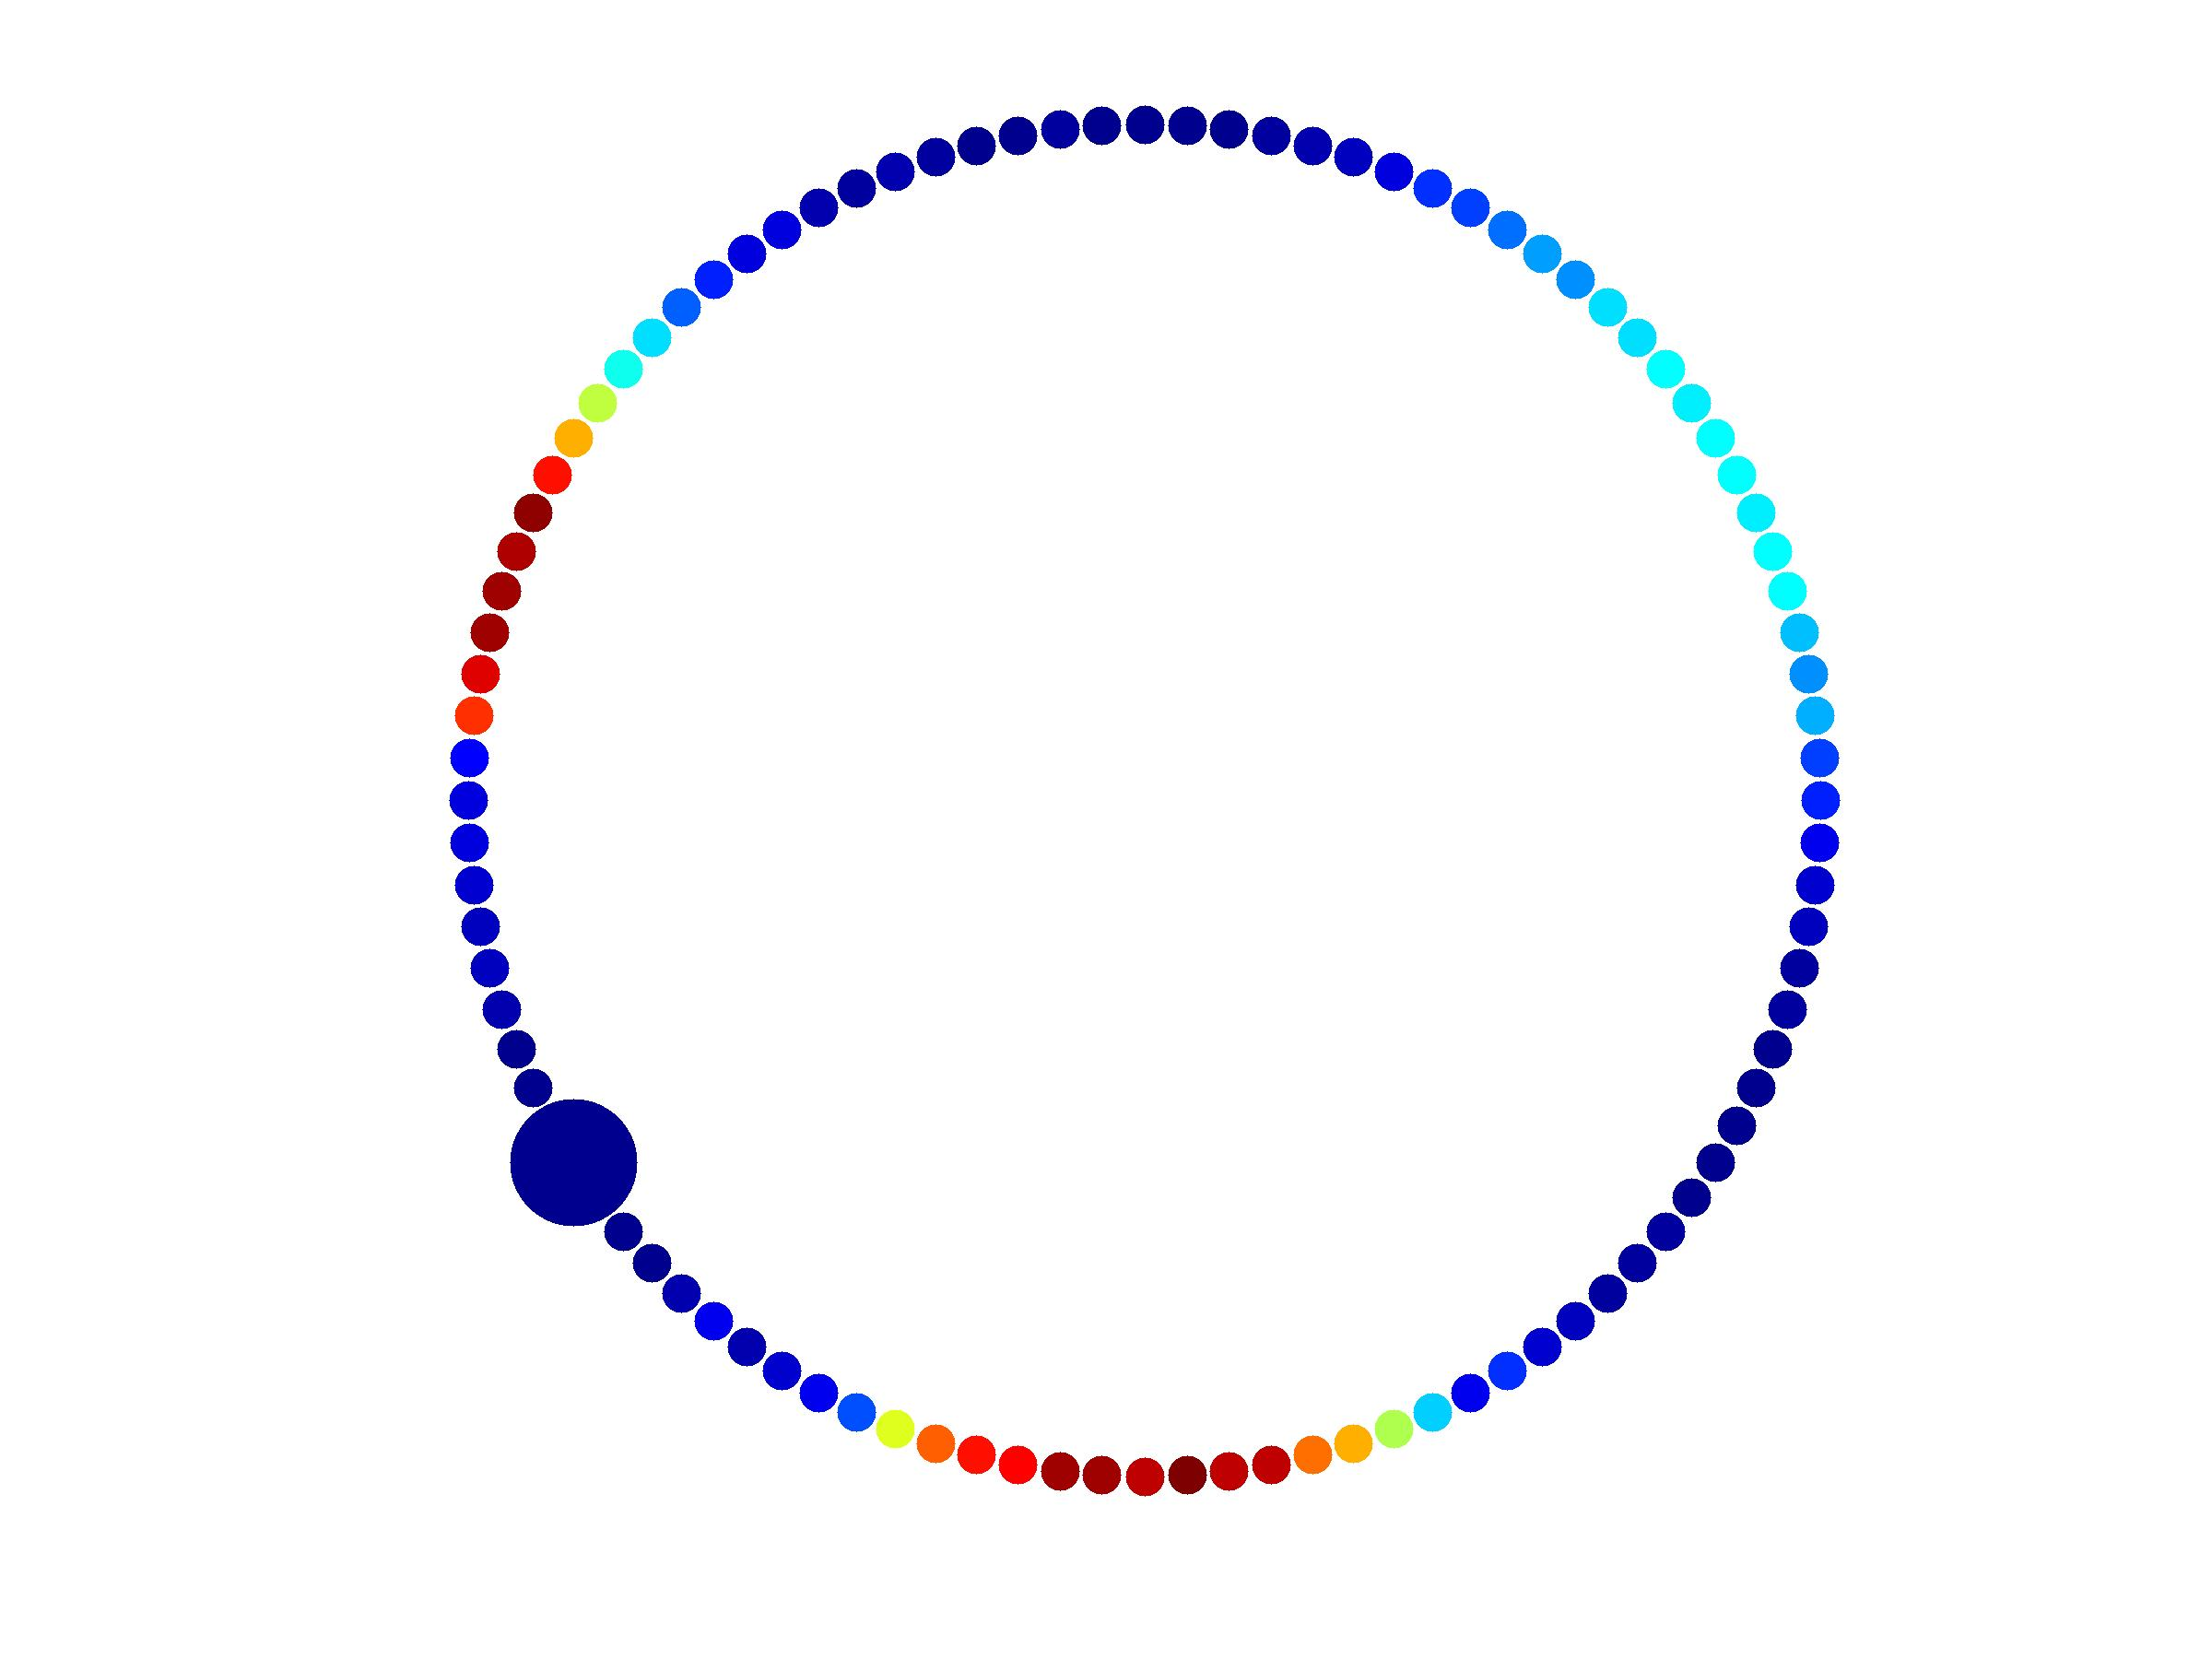
\includegraphics[width=0.45\textwidth]{../SIAM_DS_2013/drosophila_rot1.jpg}
            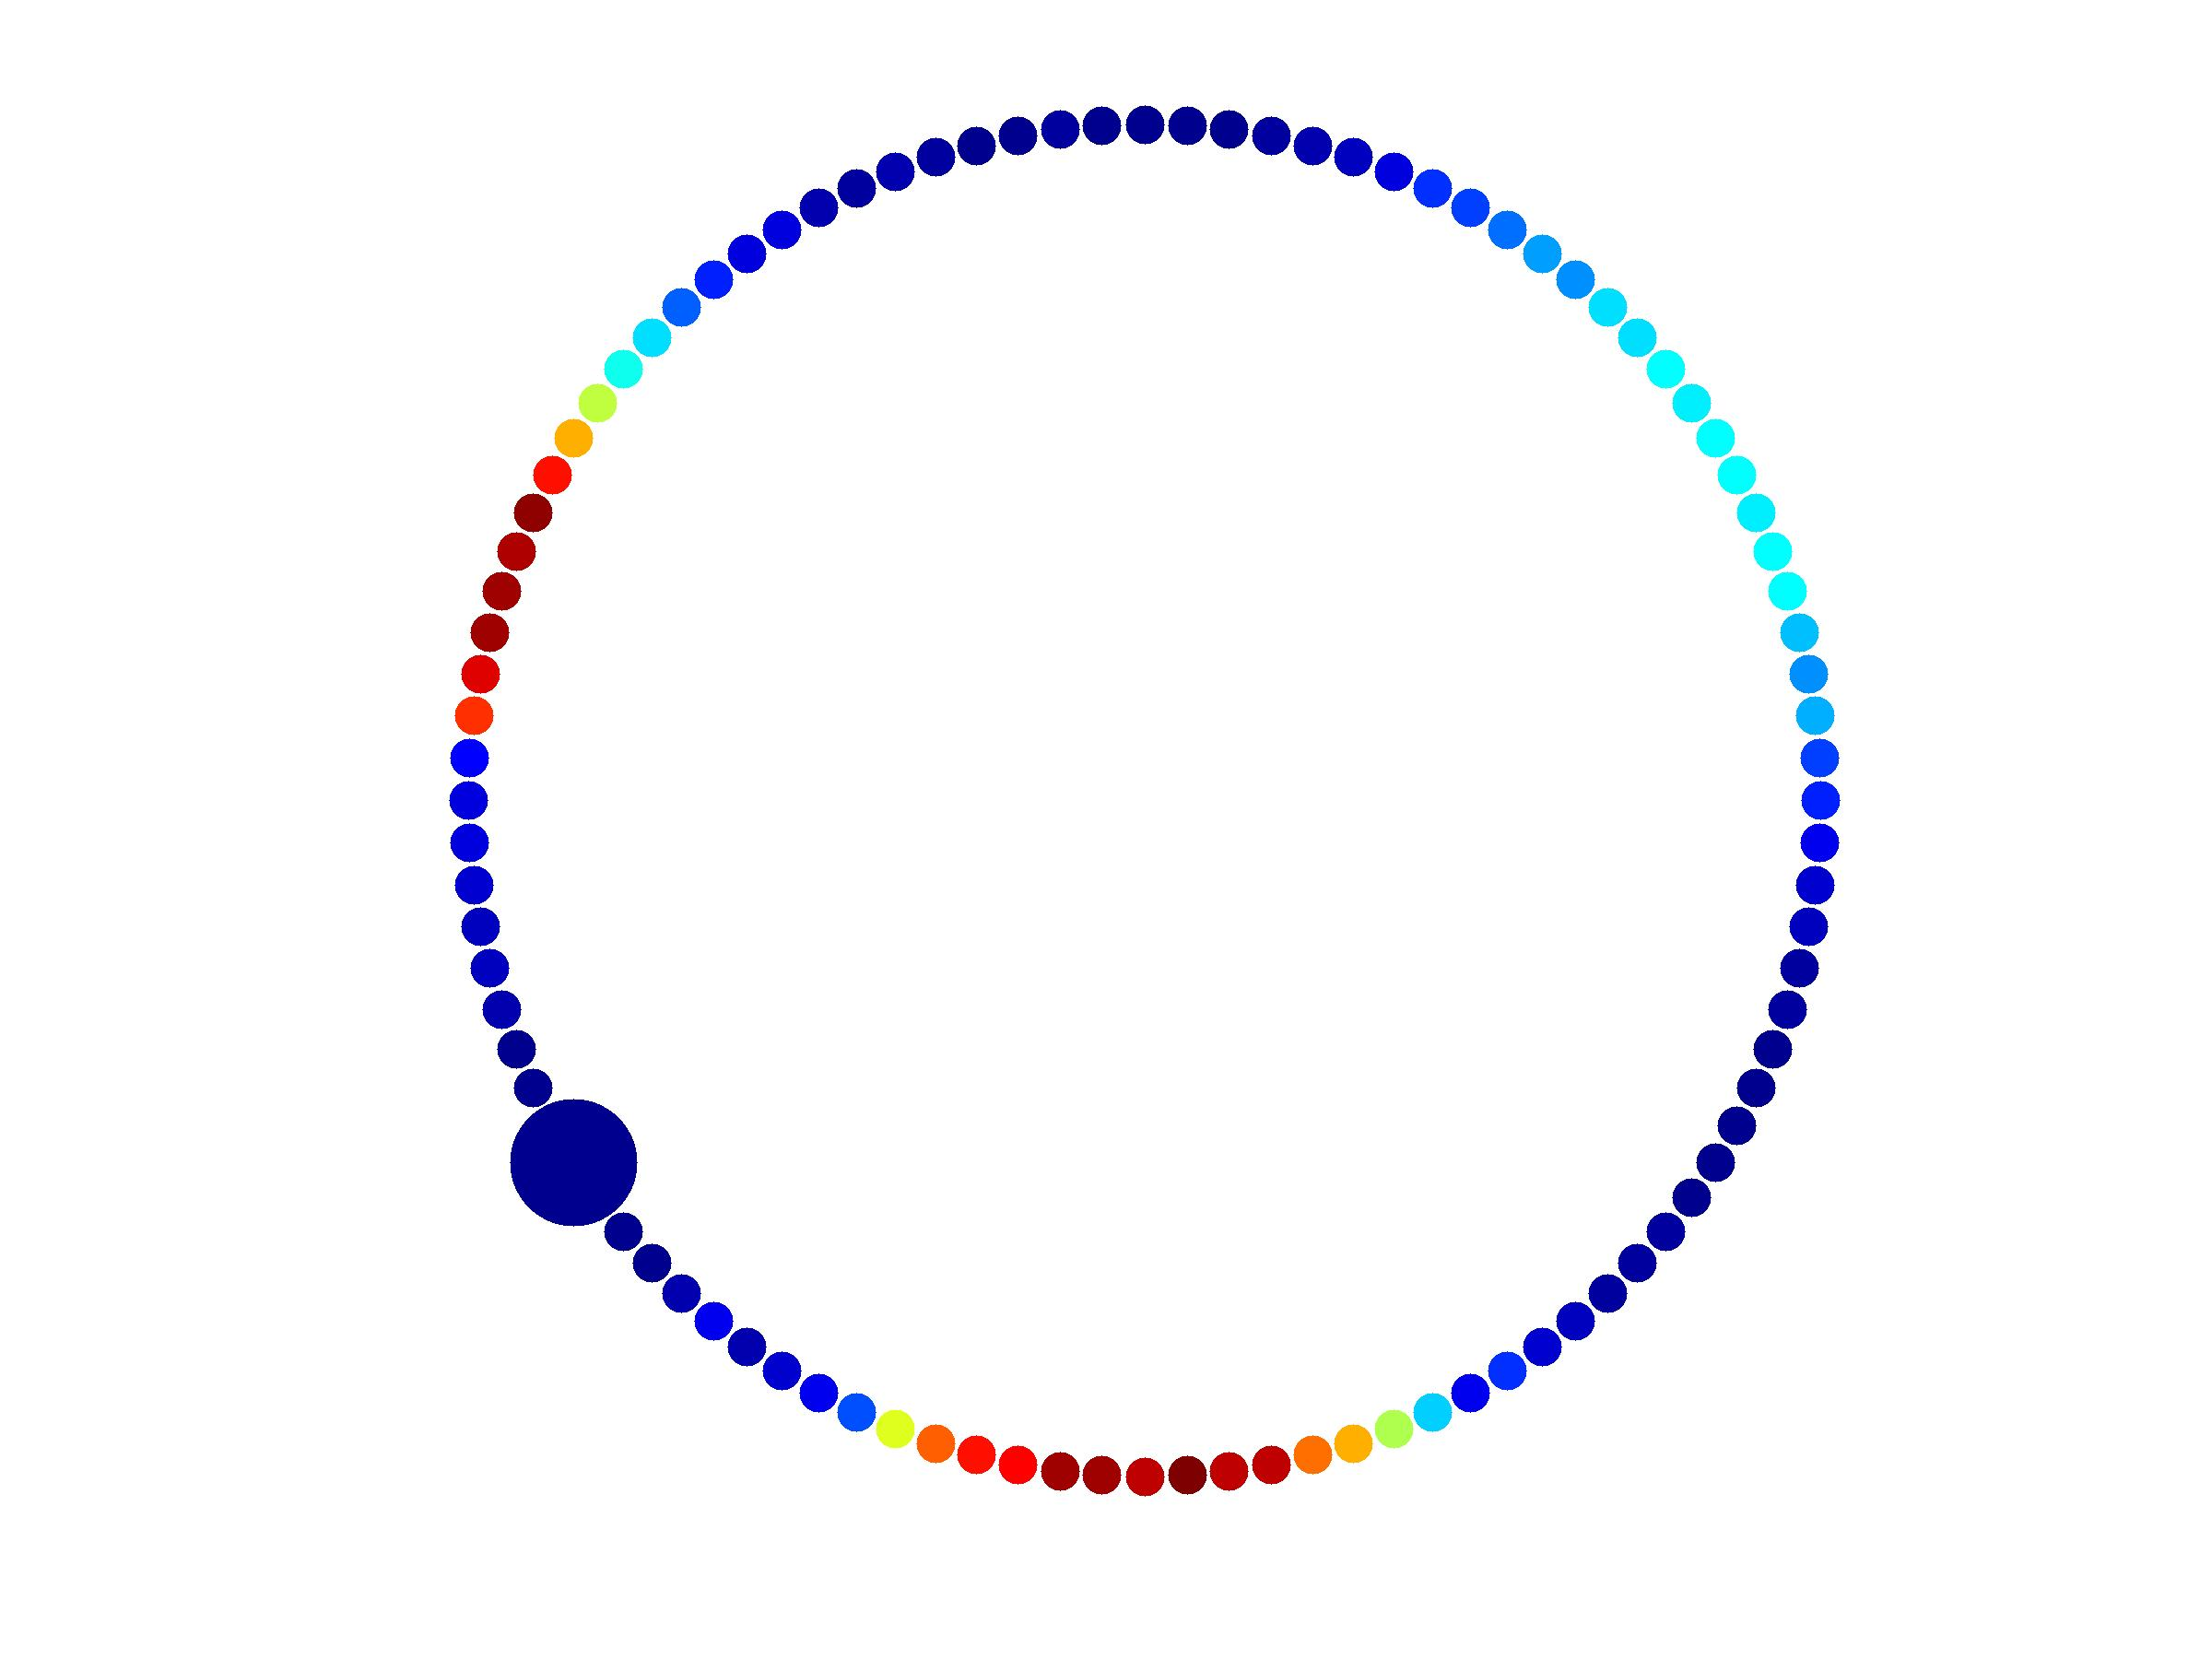
\includegraphics[width=0.45\textwidth]{../SIAM_DS_2013/drosophila_rot1.jpg}
            \end{minipage}};
            \draw [->] (fig1.east) -- (fig2.west);
        \end{tikzpicture}
	\end{block}

    We will {\bf reduce} the data by factoring out the underlying rotations
\end{frame}

\begin{frame}{Factoring Out Rotations}
    
    There are two main methods for factoring out rotations in data analysis
    \vfill
    
    \begin{columns}
	\begin{column}{0.5\textwidth}
	{\bf Template-based methods}\\
	{\small All data points are aligned to one template \par}
	\centering
		\begin{tikzpicture}
			\node (data1) {\includegraphics[width=0.2\textwidth]{../SIAM_DS_2013/drosophila_rot1_trim.jpg}};
			\node [right=0in of data1] (data2) {\includegraphics[width=0.2\textwidth]{../SIAM_DS_2013/drosophila_rot3_trim.jpg}};
			\node [right=0in of data2] (data3) {\includegraphics[width=0.2\textwidth]{../SIAM_DS_2013/drosophila_rot5_trim.jpg}};
			\node [right=0in of data3] (data4) {\includegraphics[width=0.2\textwidth]{../SIAM_DS_2013/drosophila_rot6_trim.jpg}};

			\path (data1) -- (data4) node[pos=.5,above=1in] (template) {\includegraphics[width=0.3\textwidth]{../SIAM_DS_2013/drosophila_rot1_trim.jpg}};
			\node [below=0in of template] (text1) {{\small Select a template \par}};
			
			\node[below=0in of data1]{{\scriptsize \em Data 1}};
			\node[below=0in of data2]{{\scriptsize \em Data 2}};
			\node[below=0in of data3]{{\scriptsize \em Data 3}};
			\node[below=0in of data4]{{\scriptsize \em Data 4}};
			
			\draw[<->] (text1) -- (data1) node [midway, above, sloped] {{\scriptsize Align}};
			\draw[<->] (text1) -- (data2) node [midway, above, sloped] {{\scriptsize Align}};
			\draw[<->] (text1) -- (data3) node [midway, above, sloped] {{\scriptsize Align}};
			\draw[<->] (text1) -- (data4) node [midway, above, sloped] {{\scriptsize Align}};
        \end{tikzpicture}
    \end{column}
    
    \begin{column}{0.5\textwidth}
    {\bf Angular Synchronization}\\
    {\small We calculate all pairwise alignments and then find the most {\em consistent} set of global alignments \par}
    \centering
    	\begin{tikzpicture}
    		\node (data1) {\includegraphics[width=0.2\textwidth]{../SIAM_DS_2013/drosophila_rot1_trim.jpg}};
			\node [right=of data1] (data2) {\includegraphics[width=0.2\textwidth]{../SIAM_DS_2013/drosophila_rot3_trim.jpg}};
			\node [below=of data1] (data3) {\includegraphics[width=0.2\textwidth]{../SIAM_DS_2013/drosophila_rot5_trim.jpg}};
			\node [right=of data3] (data4) {\includegraphics[width=0.2\textwidth]{../SIAM_DS_2013/drosophila_rot7_trim.jpg}};
			
			\node[below=0in of data1](text1){{\scriptsize \em Data 1}};
			\node[below=0in of data2](text2){{\scriptsize \em Data 2}};
			\node[below=0in of data3](text3){{\scriptsize \em Data 3}};
			\node[below=0in of data4]{{\scriptsize \em Data 4}};
			
			\draw[<->] (data1) -- (data2) node [midway, above, sloped] {{\scriptsize Align}};
			\draw[<->] (text1) -- (data3) node [midway, above, sloped] {{\scriptsize Align}};
			\draw[<->] (data1) -- (data4);% node [midway, above, sloped] {{\scriptsize Align}};
			\draw[<->] (data2) -- (data3);% node [midway, above, sloped] {{\scriptsize Align}};
			\draw[<->] (text2) -- (data4) node [midway, above, sloped] {{\scriptsize Align}};
			\draw[<->] (data3) -- (data4) node [midway, above, sloped] {{\scriptsize Align}};
		\end{tikzpicture}
		
		{\small {\bf In the presence of noise}, synchronization is often more robust \par}
	\end{column}
	\end{columns}
    
    %We will look at {\bf synchronization}
\end{frame}

\begin{frame}{Angular Synchronization \let\thefootnote\relax\footnote{\cite{singer2011angular}}}

	To synchronize images/concentrations on a circle under rotations in the plane:
    {\scriptsize
    \begin{itemize}
        \item We have {\bf data} $x_1, x_2, \dots, x_n$ (in our example, $x_i$ is the concentration profile of dpERK on a ring)
        % which is invariant under some group $G$

        %\item We will take $G = SO(2)$, but other symmetry groups can also be considered

        \item Let $\theta_{ij}$ denote the {\bf angle of rotation} that best aligns $x_i$ and $x_j$ (so $\theta_{ji} = -\theta_{ij}$)

        \item We seek $\hat{\theta_1}, \hat{\theta_2}, \dots, \hat{\theta_n}$ so that rotating each data point $x_i$ by $\theta_i$ will result in the most ``consistent'' aligned data

        \item We {\bf construct the matrix} $H$, where $H_{ij} = e^{i \theta_{ij}}$.

        \item We then want to solve the {\bf optimization problem}
        $$ \max_{\theta_1, \dots, \theta_n \in [0, 2\pi)} \sum_{i=1}^{n}\sum_{j=1}^{n} e^{-i \theta_i}H_{ij} e^{i \theta_j}$$


        %\item Note that if $\theta_{ij}$ is an accurate measurement, then
        %$e^{-i \theta_i}H_{ij} e^{i \theta_j} = e^{-i \theta_i}e^{i (\theta_i-\theta_j)} e^{i \theta_j} = 1$

        %\item However, if $\theta_{ij}$ is inaccurate, then $e^{-i \theta_i}H_{ij} e^{i \theta_j}$ will be a (uniform) random complex number of unit norm; these terms will (mostly) cancel

        \item We {\bf relax} the problem to
        $$\max_{z_1, \dots, z_n \in \mathbb{C}} \sum_{i=1}^{n}\sum_{j=1}^{n} \overline{z_i} H_{ij} z_j $$
%    \end{itemize}
%    \par}
%\end{frame}

%\begin{frame}{Angular Synchronization \let\thefootnote\relax\footnote{\cite{singer2011angular}}}
%
%    {\scriptsize
%    \begin{itemize}
        \item The solution to
        $$\max_{z_1, \dots, z_n \in \mathbb{C}} \sum_{i=1}^{n}\sum_{j=1}^{n} \overline{z_i} H_{ij} z_j = \max \overline{z} H z$$
        is given by $v_1$, the {\bf top eigenvector} of $H$

        \item Note that the entries of $v_1$ are not necessarily of unit norm\\
        Therefore, the optimal rotations $\hat{\theta_1}, \dots, \hat{\theta_n}$ are given by
        $e^{i \hat{\theta_i}} = \frac{v_1(i)}{|v_1(i)|}$

%        \item
%        Under a uniform noise model, the matrix $H$ can be shown to have an eigenvalue spectrum that consists of a semicircle distribution \footcite{wigner1955characteristic, wigner1958distribution}, with one outlier corresponding to the top eigenvector, which contains the optimal alignments\\
%        \begin{center}
%        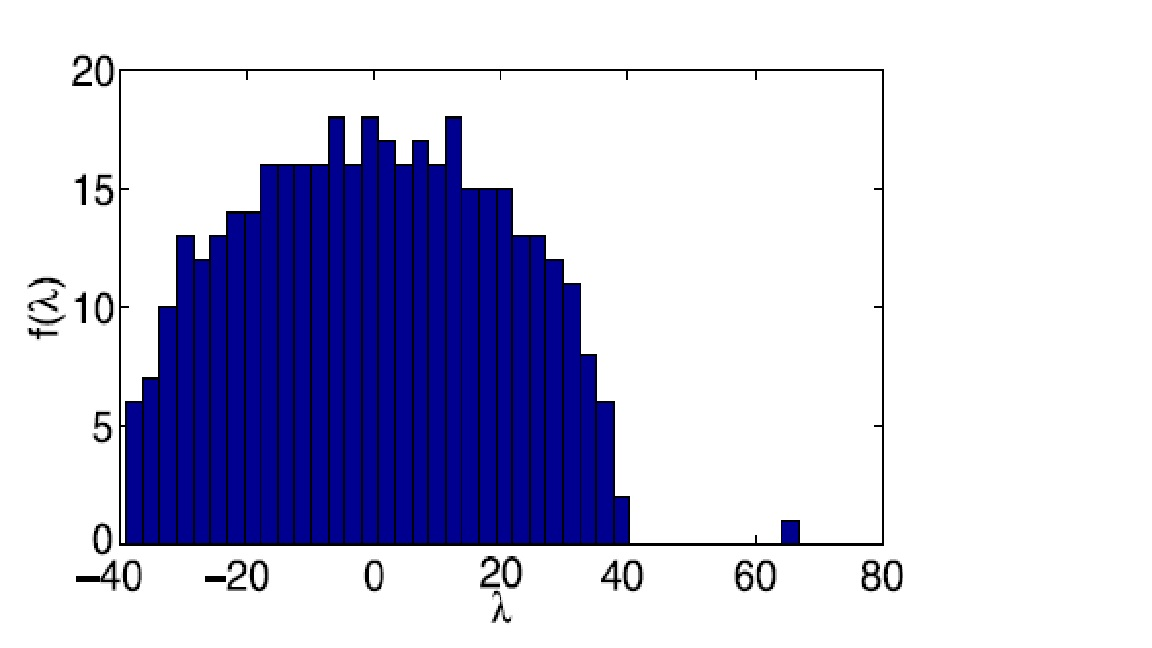
\includegraphics[width=0.3\textwidth]{../SIAM_DS_2013/evec_spectrum.jpg}
%        \end{center}
%
%        \item Also note that this formulation takes into account {\em consistency}\\
%        For example, if we want to satisfy two angle relations $\theta_i-\theta_k \approx \theta_{ij} + \theta_{jk} \forall j$, we would solve
%        $$\max_{z_1, \dots, z_n \in \mathbb{C}} \sum_{i=1}^{n}\sum_{k=1}^{n} \overline{z_i} \left( \sum_{j=1}^{n} e^{i (\theta_{ij} + \theta_{jk})} \right) z_k = \max \overline{z} H^2 z$$
%
%        The solution to this optimization problem is also $v_1$, the top eigenvector of $H$
    \end{itemize}
    \par}
\end{frame}

\begin{frame}{Alignment Results}

	We can use angular synchronization to align the concentration profiles {\em even~before} ordering the profiles in time
	
	\begin{tikzpicture}
		\node[] (fig1) {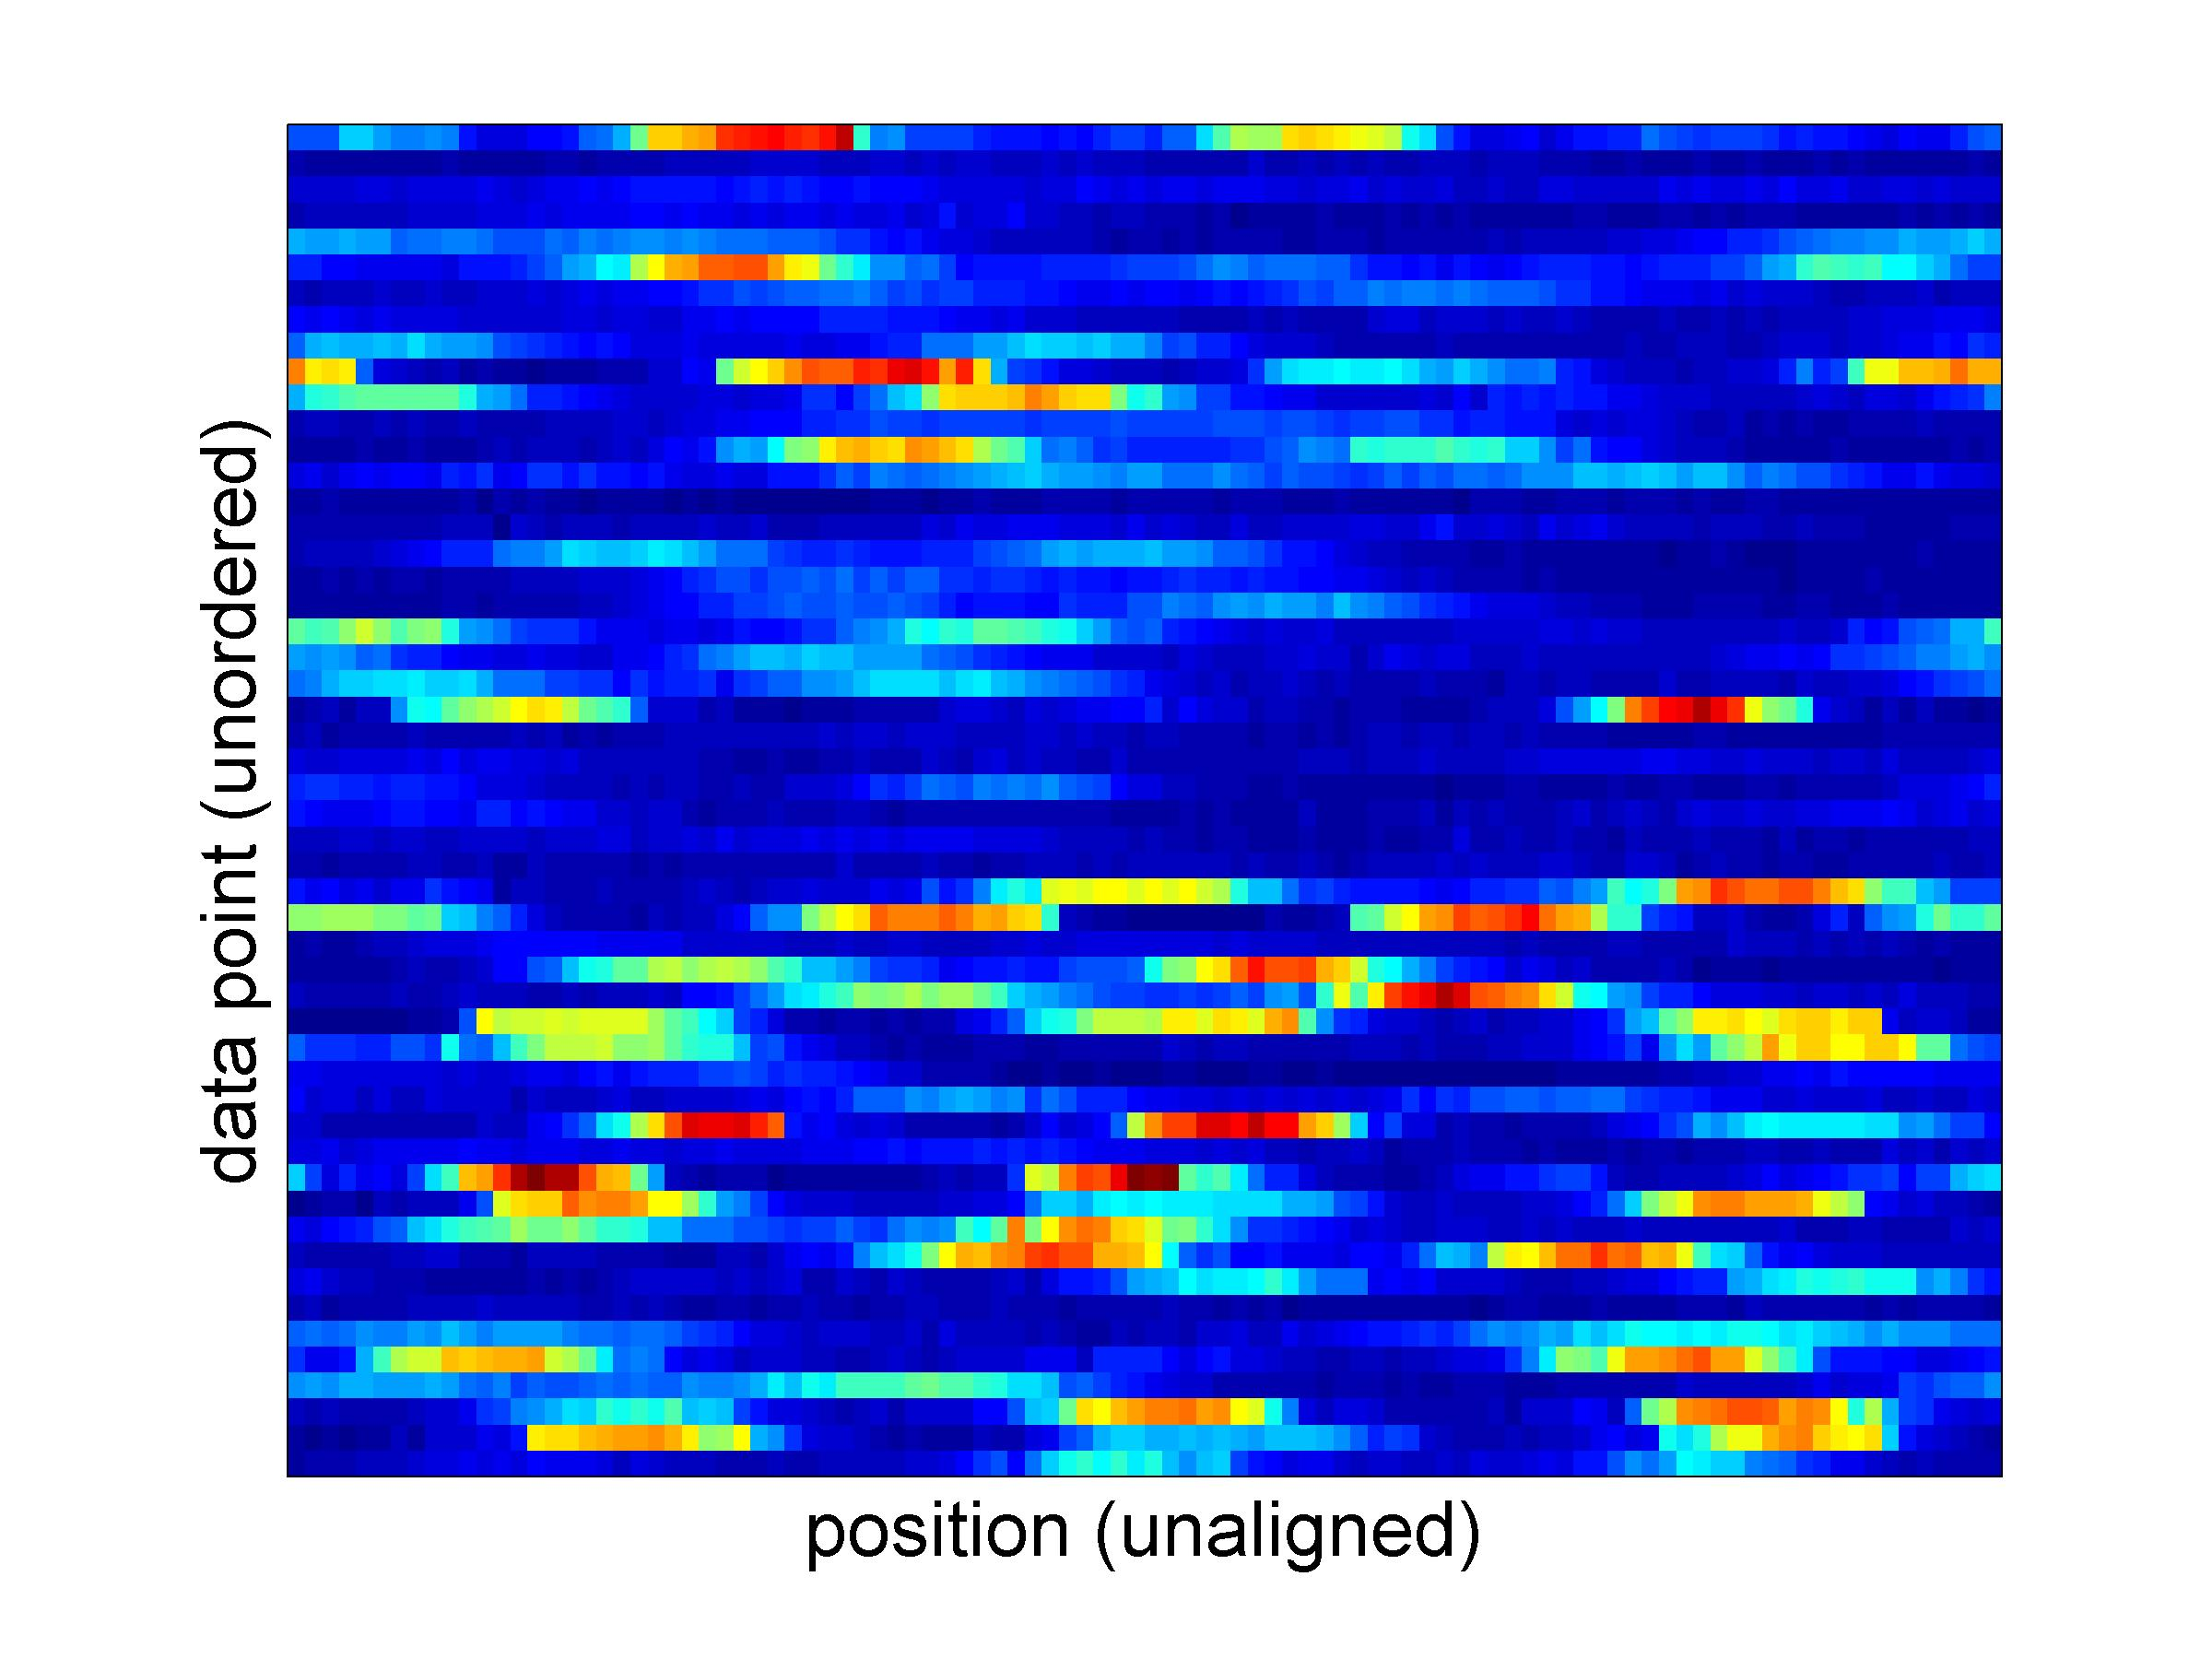
\includegraphics[width=0.25\textwidth]{data_unaligned_unordered}};
		\node[right of=fig1, node distance=0.3\textwidth] (fig2) {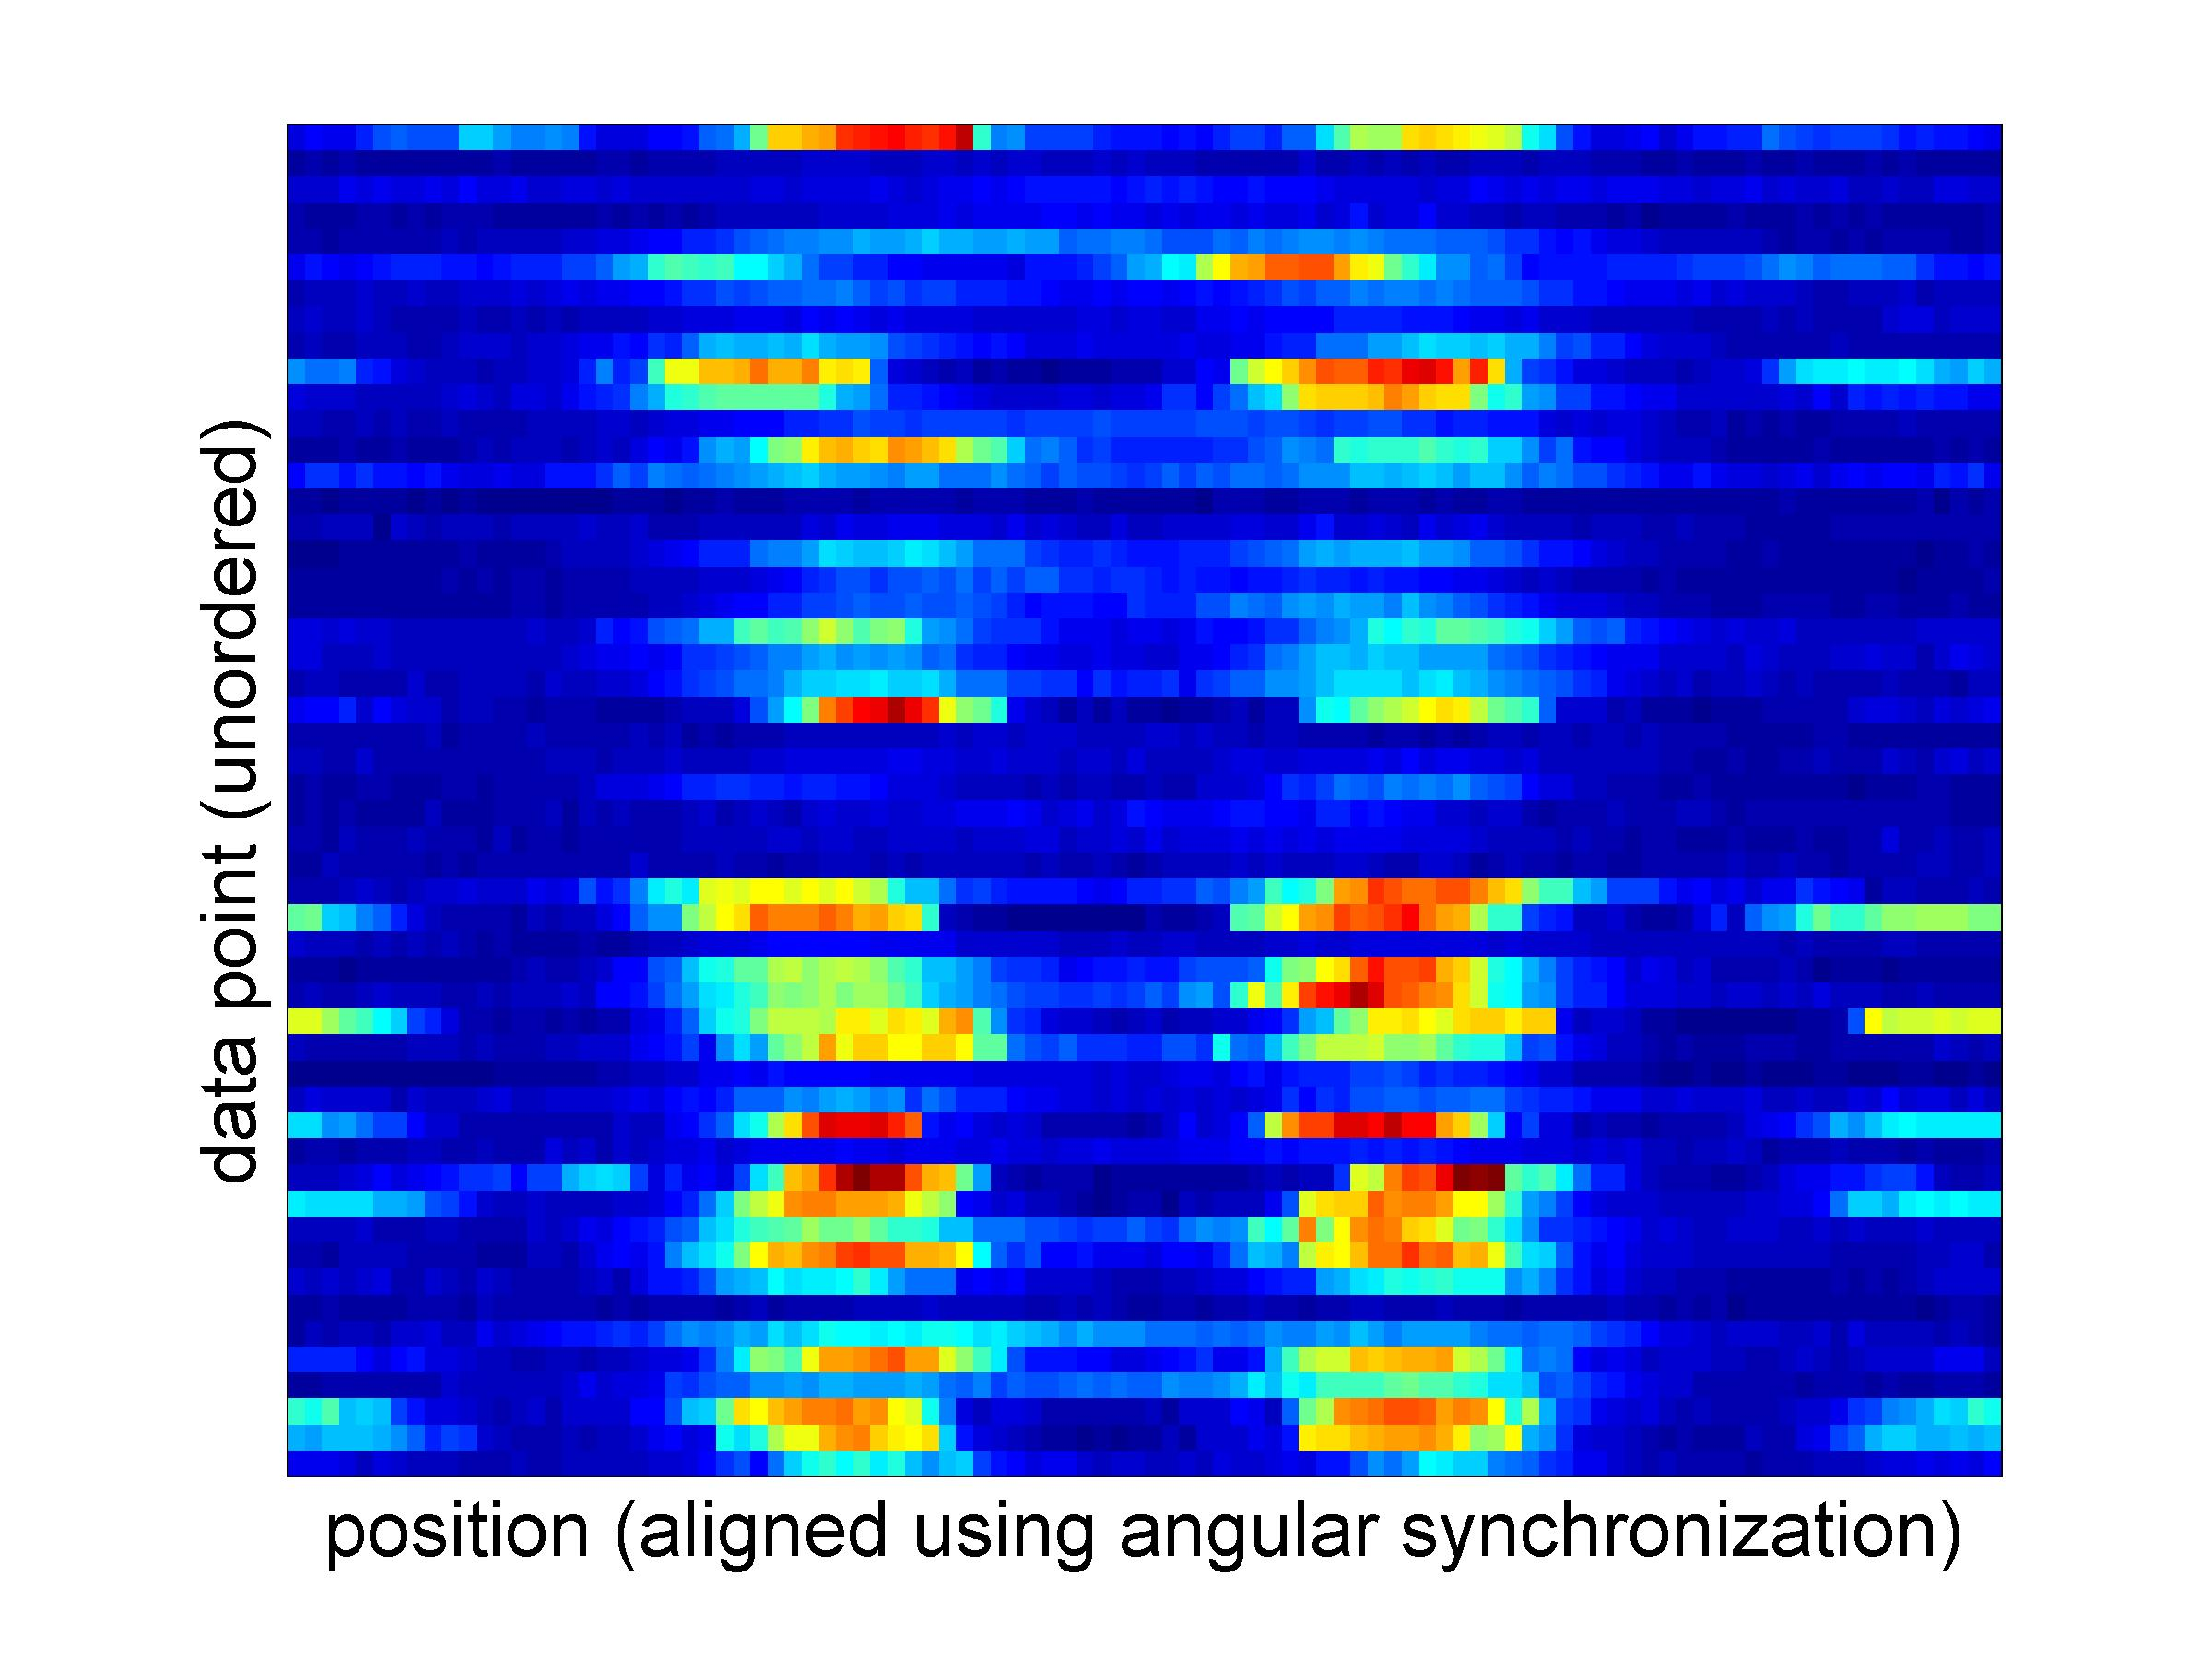
\includegraphics[width=0.25\textwidth]{data_aligned_unordered}};
		\node[right of=fig2, node distance=0.3\textwidth] (fig3) {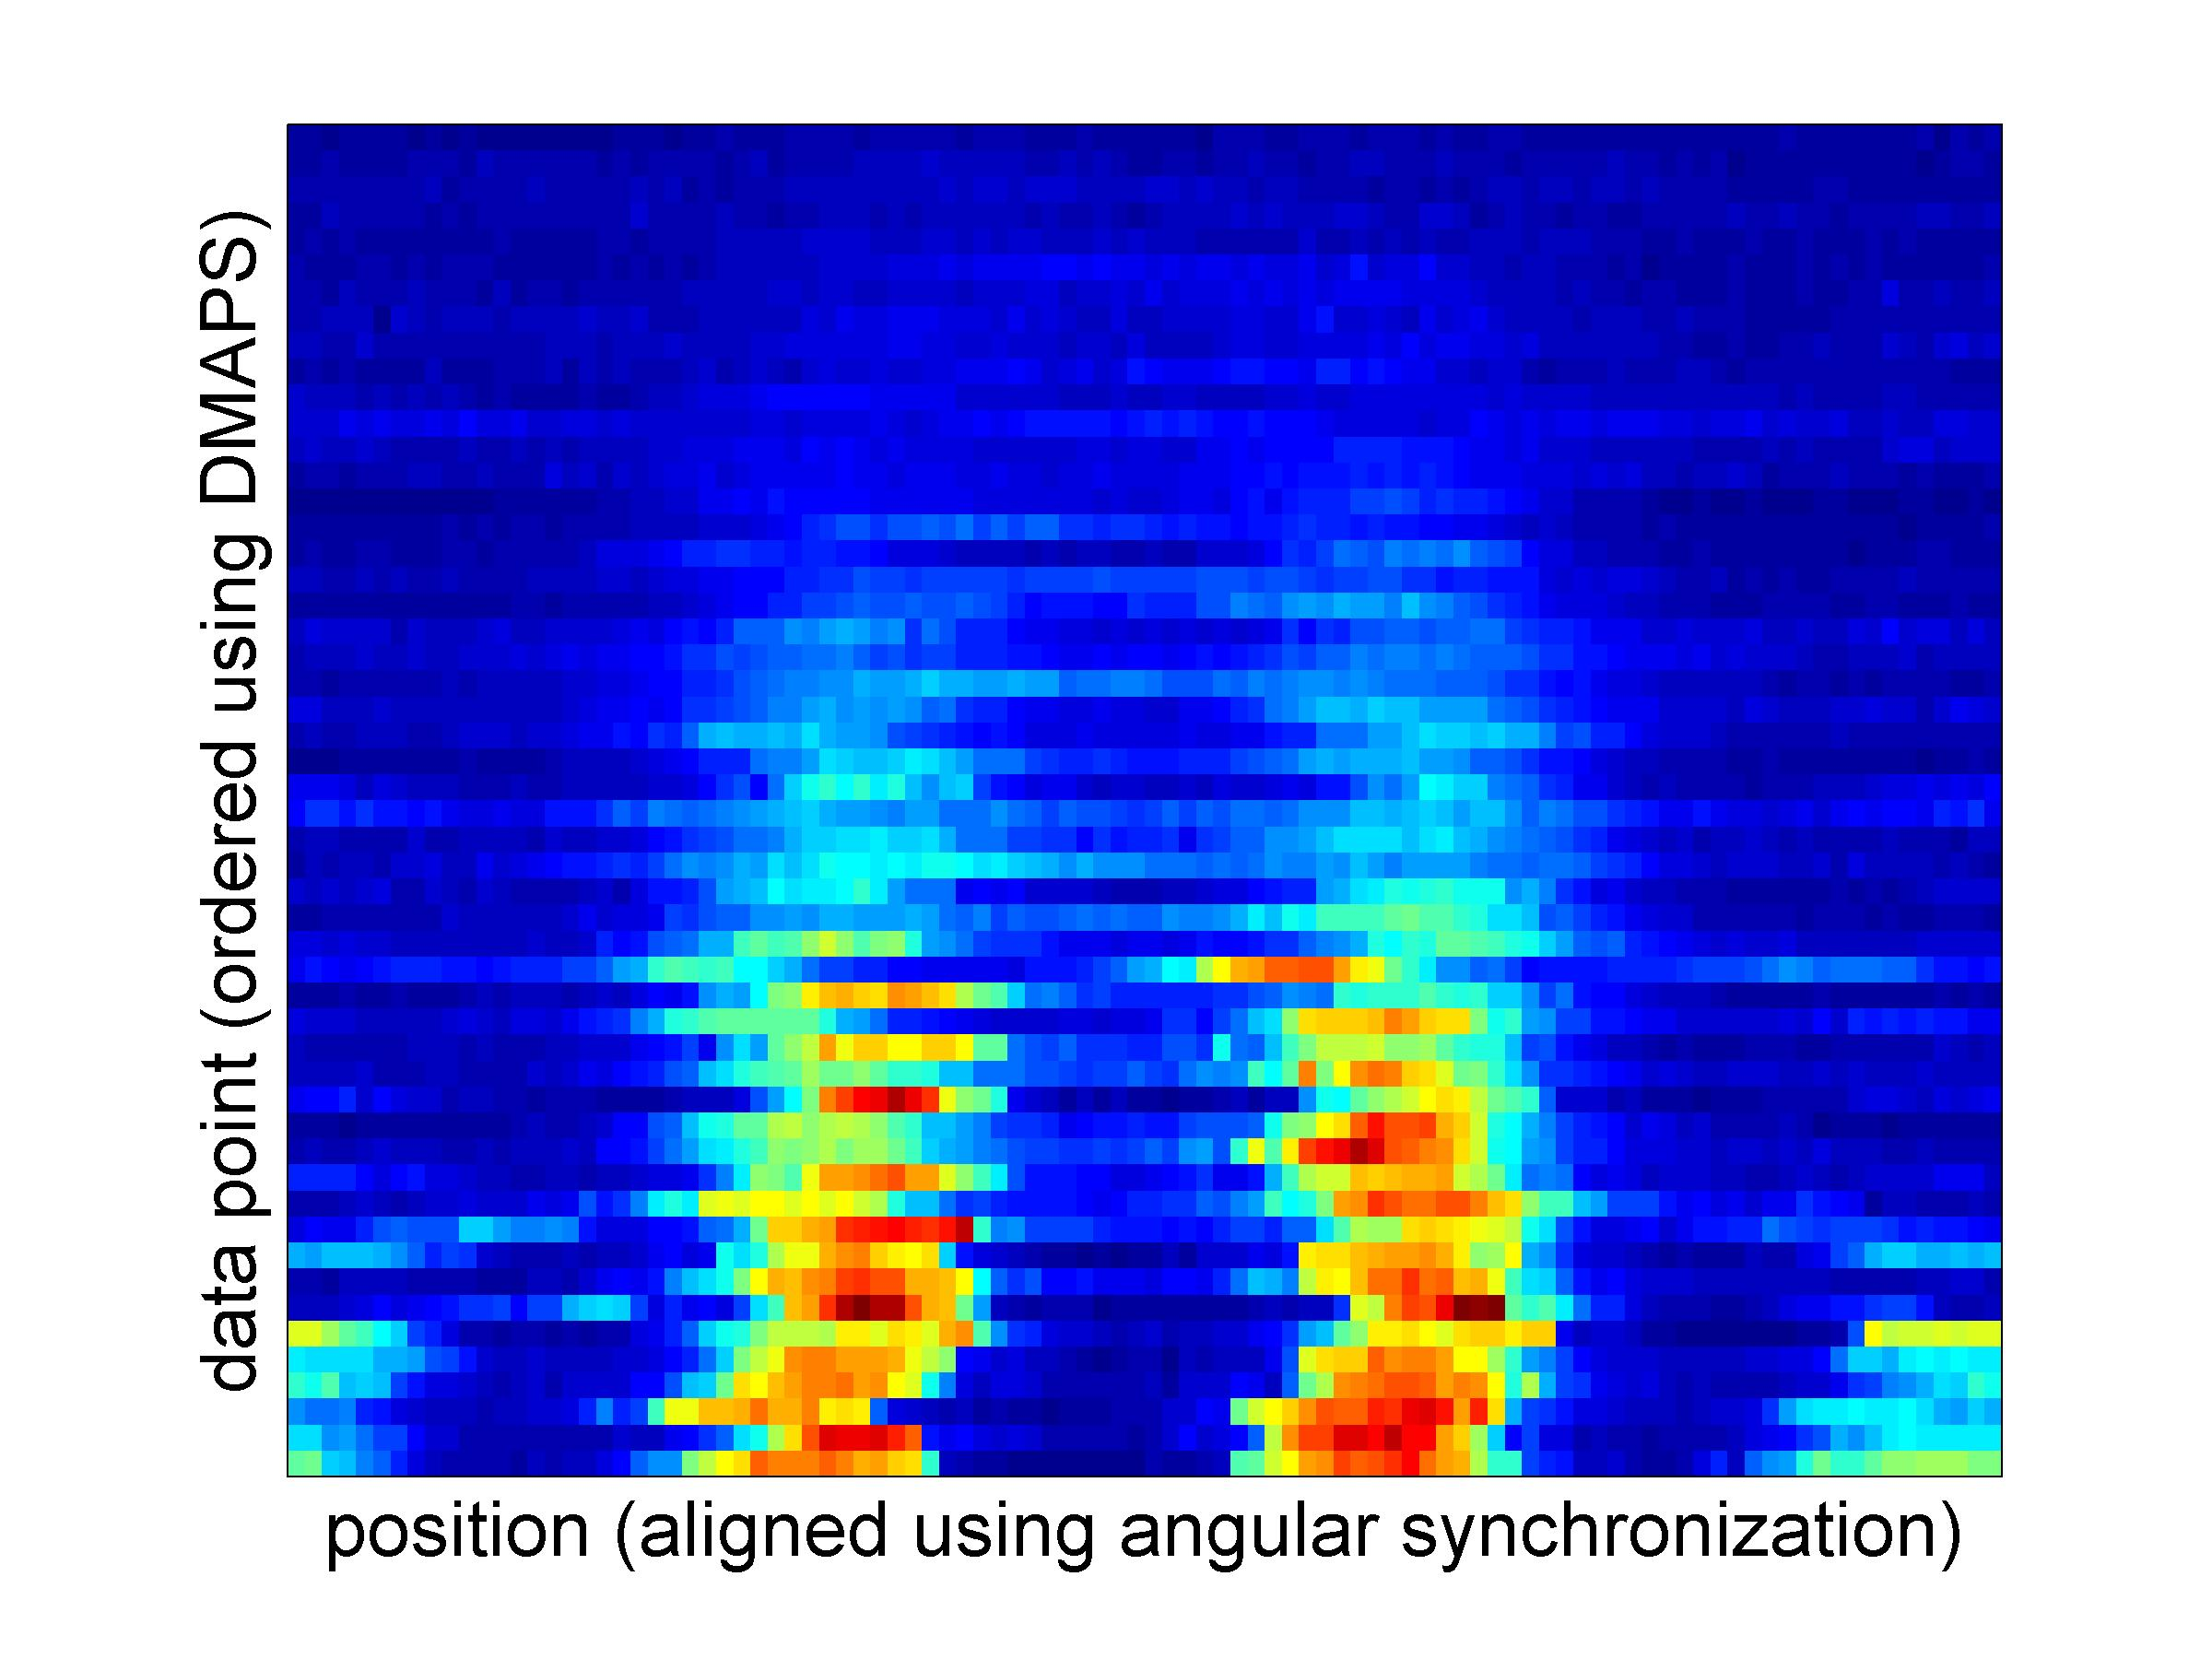
\includegraphics[width=0.25\textwidth]{data_ordered_angsynch}};
		\draw[->] (fig1.east) -- (fig2.west);
		\draw[->] (fig2.east) -- (fig3.west);
		\node[below of=fig1, node distance=1in, text width=0.3\textwidth]{{\small Profiles are unaligned and unordered}};
		\node[below of=fig2, node distance=1in, text width=0.3\textwidth]{{\small Profiles are aligned using angular synchronization but temporally unordered}};
		\node[below of=fig3, node distance=1in, text width=0.3\textwidth]{{\small Profiles are then ordered in time}};
	\end{tikzpicture}

\end{frame}

\begin{frame}{Vector Diffusion Maps: Synchronization and Diffusion Maps}
	\begin{itemize}
		\item Our data contains both symmetries {\em and} dynamics
		\item We would like to combine angular synchronization and diffusion maps into one computation that allows us to both factor out symmetries and order the data
	\end{itemize}
\end{frame}

\begin{frame}{Align and Order using Vector Diffusion Maps}

	\centering
	We can use vector diffusion maps to align {\em and} order the profiles.

	\begin{tikzpicture}
		\node[] (fig1) {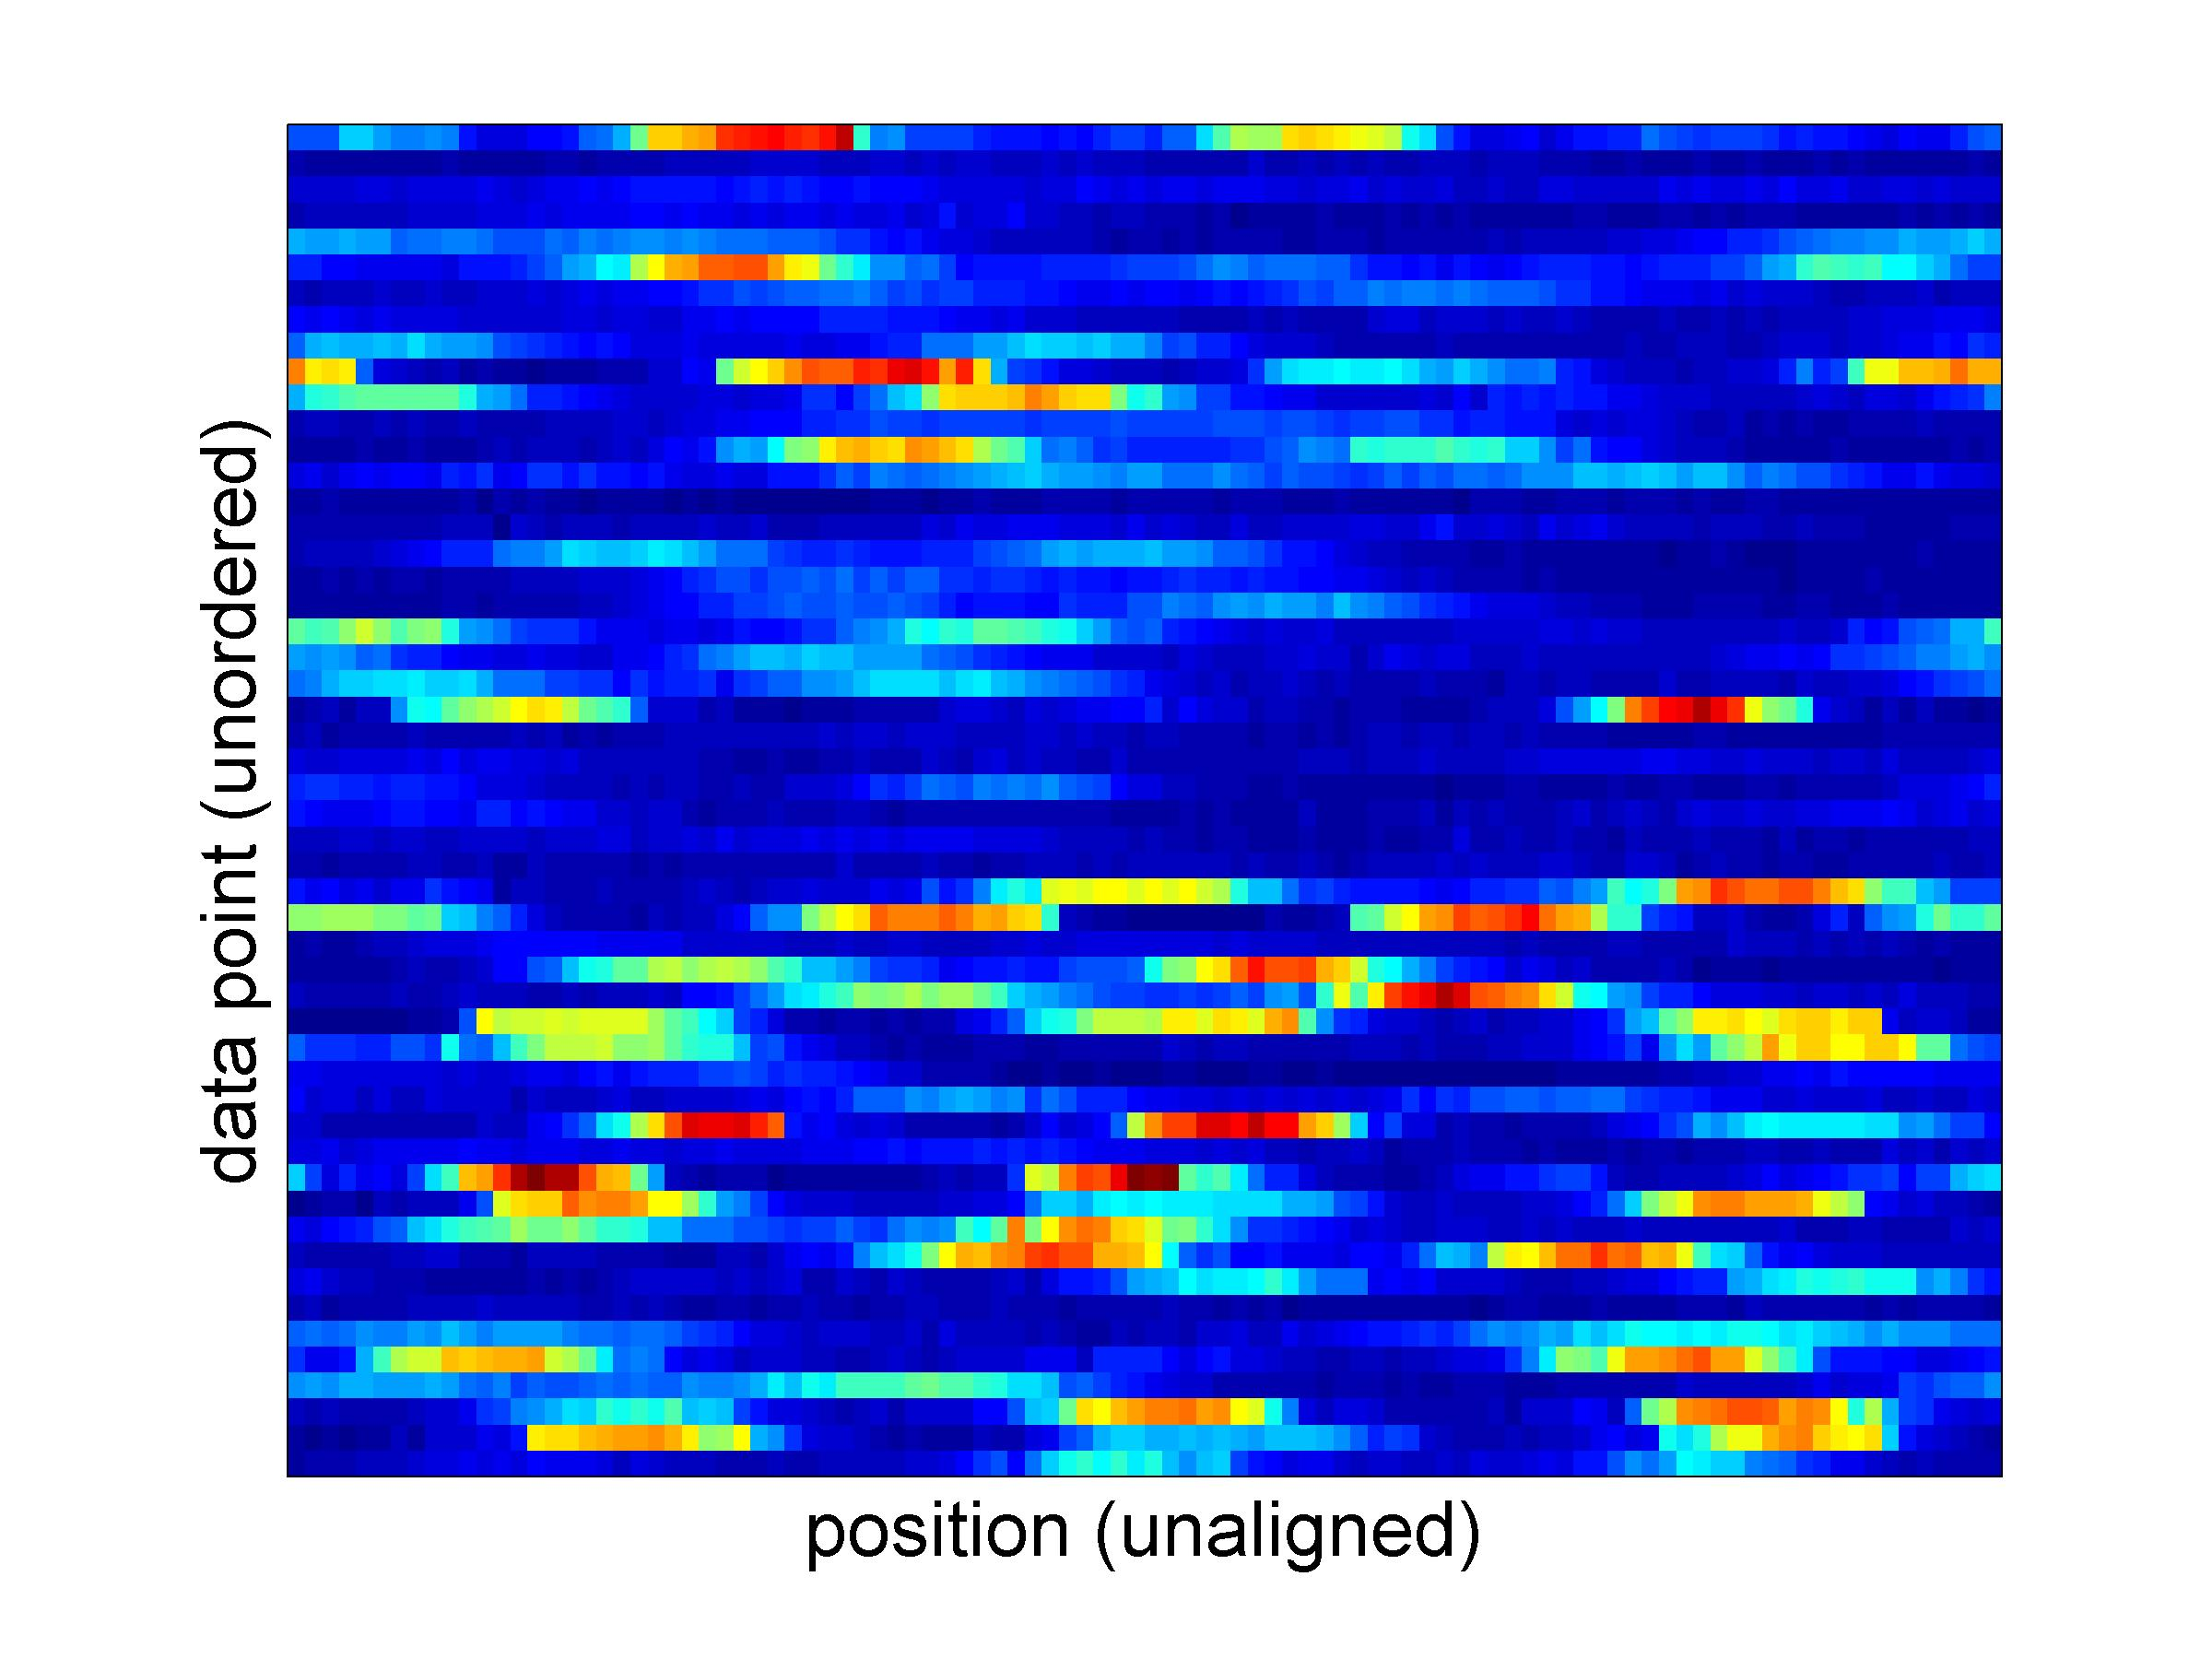
\includegraphics[width=0.4\textwidth]{data_unaligned_unordered}};
		\node[right of=fig1, node distance=0.5\textwidth] (fig2) {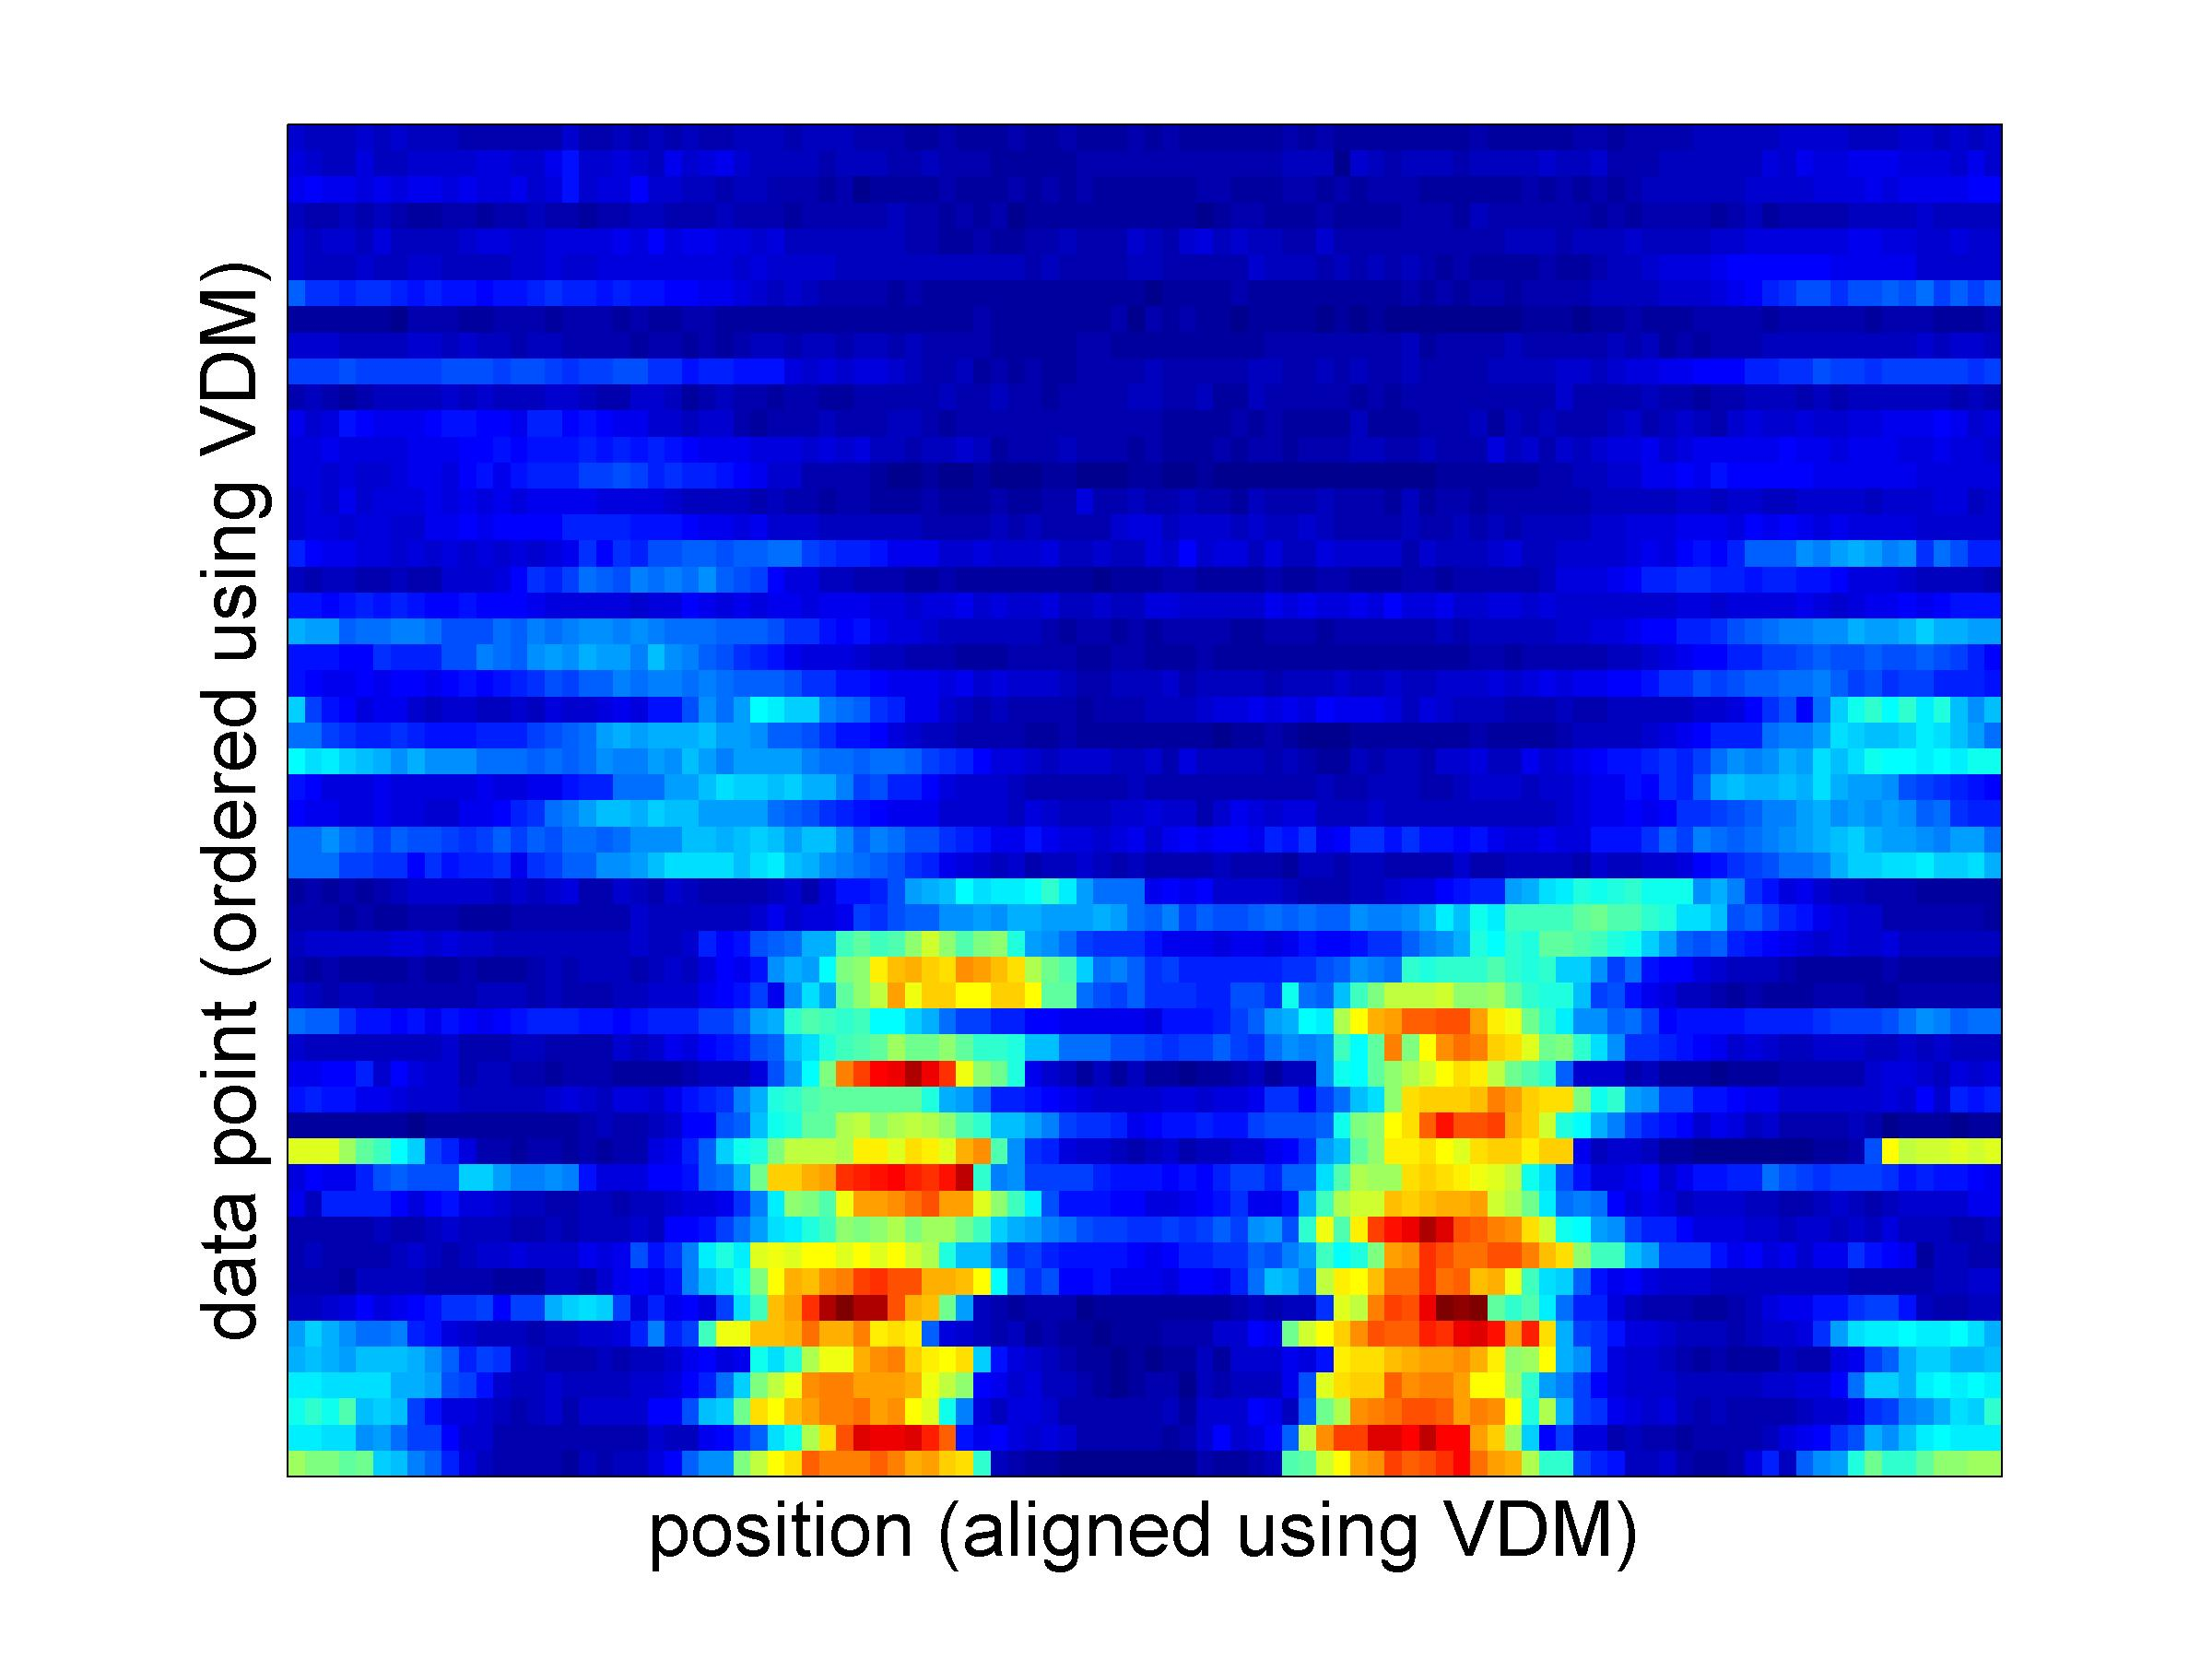
\includegraphics[width=0.4\textwidth]{data_ordered_vdm}};
		\draw[->] (fig1.east) -- (fig2.west);
		\node[below of=fig1, node distance=1in, text width=0.4\textwidth]{{\small Profiles are unaligned and unordered}};
		\node[below of=fig2, node distance=1in, text width=0.4\textwidth]{{\small Profiles are aligned and ordered using vector diffusion maps}};
	\end{tikzpicture}
	
	\centering
	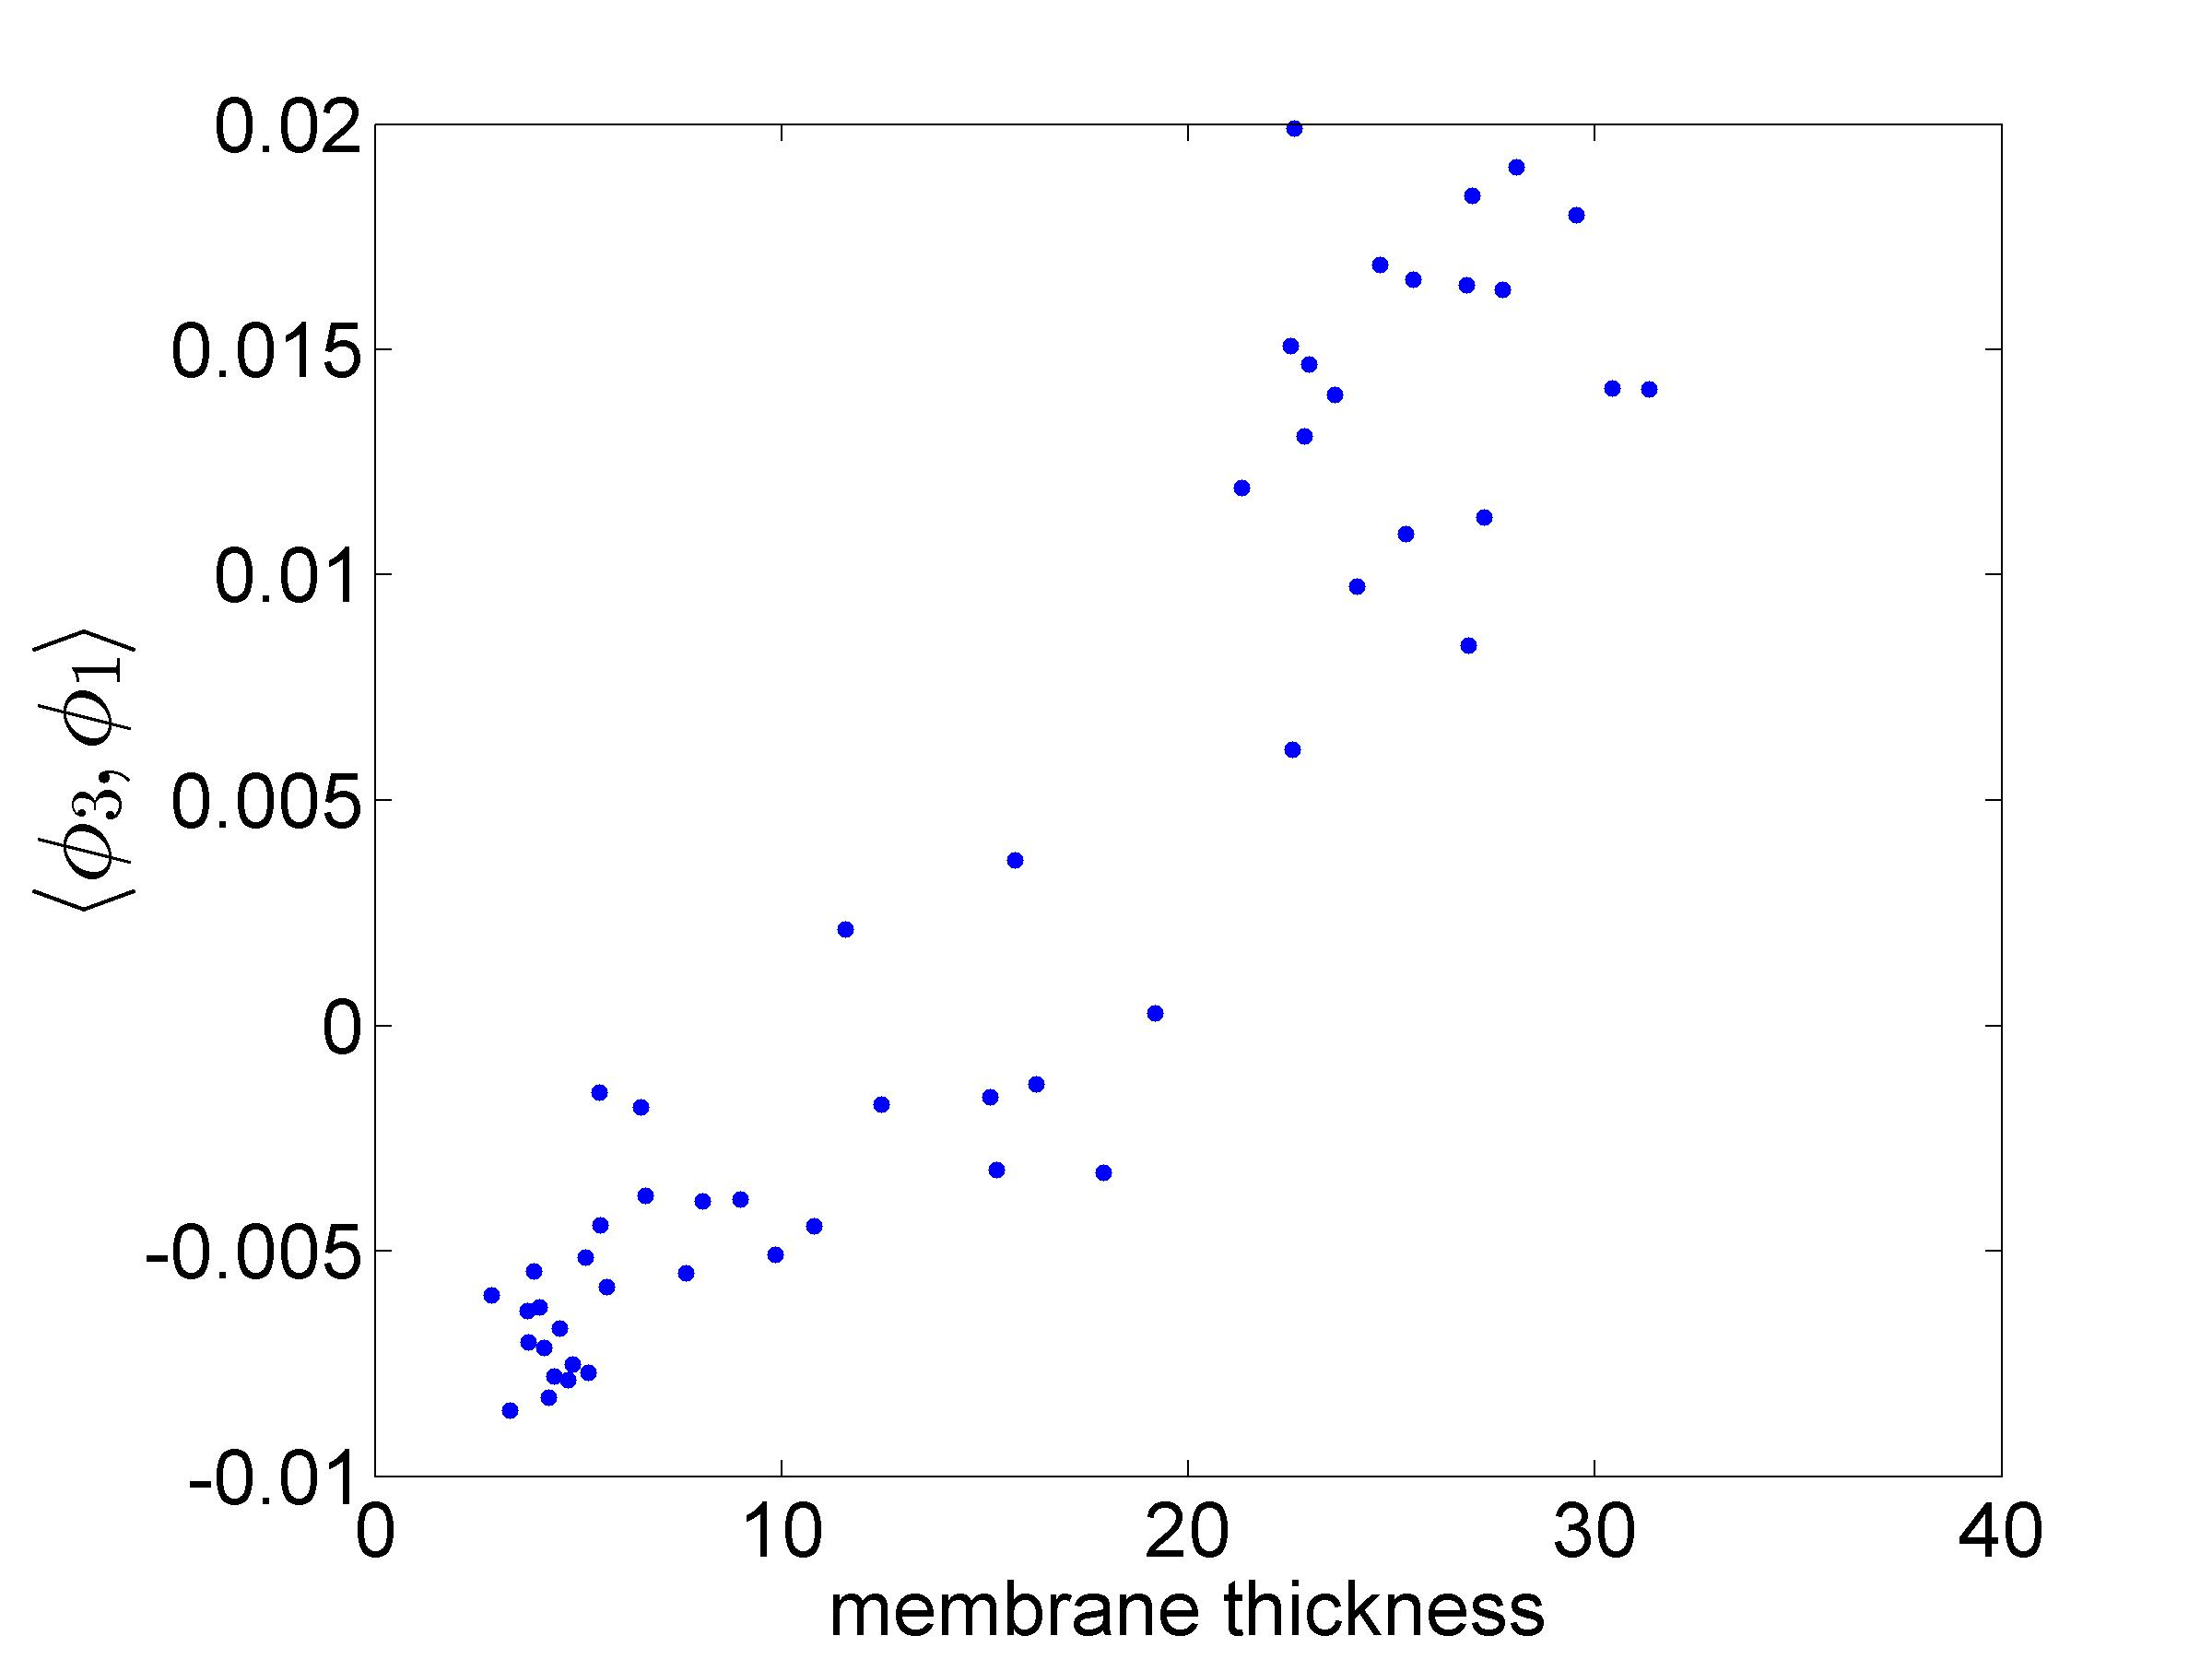
\includegraphics[width=0.4\textwidth]{VDM_time_corr}	

\end{frame}